\documentclass{VUMIFPSmagistrinis}
\usepackage{algorithmicx}
\usepackage{algorithm}
\usepackage{algpseudocode}
\usepackage{amsfonts}
\usepackage{amsmath}
\usepackage{bm}
\usepackage{caption}
\usepackage{color}
\usepackage{float}
\usepackage{graphicx}
\usepackage{listings}
\usepackage{subfig}
\usepackage{wrapfig}
\usepackage{multicol}
\usepackage{lscape}
\usepackage{array}
\usepackage{numprint}
\usepackage{makecell}

\captionsetup{labelsep=space}
\captionsetup[table]{labelsep=period}

\newcolumntype{X}{>{\setbox0=\hbox\bgroup}c<{\egroup}@{}}

\usepackage{siunitx}
\sisetup{
  round-mode          = places, % Rounds numbers
  round-precision     = 4, % to 2 places
  output-decimal-marker = {,}
}

% Titulinio aprašas (nereikalingus elementus užkomentuoti)
\university{Vilniaus universitetas}
\faculty{Matematikos ir informatikos fakultetas}
\department{Programų sistemų studijų programa}
\papertype{Magistro baigiamasis darbas}
\title{Bitininkystės procesų modeliavimas}
\titleineng{Modelling of Beekeeping Processes}
\author{Vytautas Vėgėlė}
% \status{2 kurso, 2 grupės studentas}
% \secondauthor{Vardonis Pavardonis}   % Pridėti antrą autorių
\supervisor{asist. dr. Tomas Plankis}
\reviewer{asist. dr. Vytautas Valaitis}
\date{Vilnius -- \the\year}

% Nustatymai
% \setmainfont{Palemonas}  % Pakeisti teksto šriftą į Palemonas (turi būti įdiegtas sistemoje)
\bibliography{bibliografija}  % Literatūros šaltinių aprašų failas bus bibliografija.bib

\begin{document}
\maketitle

\tableofcontents

% \sectionnonum{Sutartinių terminų sąrašas}
% Sutartinių ženklų, simbolių, vienetų, trumpinimų ir terminų sąrašas sudaromas
% tada, jei ženklų, simbolių, vienetų ir terminų bendras skaičius didesnis nei 10
% ir kiekvienas iš jų tekste kartojasi daugiau nei 3 kartus. 

\sectionnonumnocontent{Anotacija}
% Glaustai aprašomas darbo turinys: pristatomi darbo tikslai, analizuotos ir
% tirtos problemos, atlikti eksperimentai bei padarytos išvados, gautos
% rekomentacijos. Santraukos apimtis ne didesnė nei 0,5 puslapio. Santraukų gale
% nurodomi darbo raktiniai žodžiai. 
% Nurodomi iki 5 svarbiausių temos raktinių žodžių (terminų).
% Vienas terminas gali susidėti iš kelių žodžių.
% \raktiniaizodziai{raktinis žodis 1, raktinis žodis 2, raktinis žodis 3, raktinis žodis 4, raktinis žodis 5}
Darbe siekiama sukurti patobulintą bičių populiacijos kompiuterinį modelį. Atlikus esančių modelių analizę apjungti BEEHAVE ir Bumble-BEEHAVE modeliai, prie jų pridėtas spietimosi procesas ir aprašytas bičių migracijos procesas. Sukurtas ir išanalizuotas patobulintas greitasis besispiečiančios bičių šeimos algoritmas. Atliktas šio ir kitų dirbtinių bičių šeimų algoritmų palyginimas naudojant 25 skirtingas tikslo funkcijas ir Wilcoxon testą. Pateikta ir kita šio algoritmo versija, kuri buvo pritaikyta patobulinto modelio spietimosi procese.
\raktiniaizodziai{dirbtinis bičių šeimos algoritmas, kompiuterinis modeliavimas, bitininkystė, optimizavimo užduotys.}

\sectionnonumnocontent{Summary}
% Santrauka anglų kalba. Santraukos apimtis ne didesnė nei 0,5 puslapio.
% \keywords{keyword 1, keyword 2, keyword 3, keyword 4, keyword 5}
The purpose of this paper was to create an improved bee population computer model. After researching current bee models, two current models (BEEHAVE and Bumble-BEEHAVE) were combined. This joint model was expanded by adding a swarming process and an additional bee drifting process implementation was described. An improved quick swarming artificial bee colony algorithm was introduced and compared to currently existing artificial bee colony algorithms. 25 different goal functions for fitness evaluation and Wilcoxon signed-rank test was used to determine any statistical significance between results. Another variation of said algorithm was adopted and used in the new improved bee model to implement a swarming process.
\keywords{artificial bee colony algorithm, computer modelling, beekeeping, optimization problems.}


\sectionnonum{Įvadas}
% Įvade aprašomi darbo tikslai, nurodomas temos aktualumas, motyvacija,
% formuluojamas sprendžiamas uždavinys ir siekiami/pasiekti rezultatai.
% Aptariamos teorinės darbo prielaidos bei metodika, apibrėžiamas tiriamasis
% objektas, apibūdinami su tema susiję literatūros ar kitokie šaltiniai, temos
% analizės tvarka, darbo atlikimo aplinkybės, pateikiama žinių apie naudojamus
% instrumentus (programas ir kt.).

Bičių populiacijos kaita Europos šalyse \cite{LHC16} yra aktuali tema. Naujausi Europos komisijos tyrimai nagrinėja spartų bičių populiacijos mažėjimą bei bando paaiškinti įvairių aplinkos poveikių įtaką bičių sveikatai \cite{EFSA17a}. Didelis dėmesys skiriamas pesticidų poveikiui bitėms \cite{EFSA18} ir varozei \cite{EFSA17a}.  Dalis šių tyrimų ir projektų remia bičių stebėjimo būdus, o kompiuterinių modelių naudojimas yra pigesnė alternatyva nei visų bitynų stebėjimas. 
Bitininkystės procesams simuliuoti yra sukurtų įvairių kompiuterinių modelių skirtingais laikotarpiais \cite{BTO13}. Vienas senesnių modelių yra BEEPOP \cite{DRL89}, modeliuojantis vienos bičių šeimos (viena motinėlė su darbininkėmis ir tranais) avilyje (lizde). Šiame modelyje bičių šeima gyvena be išorinių veiksnių, galinčių pakenkti bičių šeimos populiacijai: daroma prielaida, jog aplinkui yra maisto, jų nepuola kiti gyvūnai. Šis modelis buvo papildytas varozės procesais \cite{HoC05} tik 2004 m. Vienas sudėtingiausių bičių šeimos tipo modelių yra HoPoMo \cite{ScC07}, naudojantis 65-ias diferencialines lygtis. Šio modelio trūkumas šeimos atžvilgiu yra fiksuotas bičių amžius, modelis paskiria bitėms darbus neatsižvelgiant į brandą. Šį trūkumą sprendžia Khoury modelis \cite{KBM13}, keisdamas bičių atliekamus darbus pagal jų amžių. Naujesni modeliai įprastai remiasi senesniais modeliais, sujungdami jų tiriamus procesus, pavyzdžiui, Torres‘o \cite{TRR15} sukurtas modelis simuliuoja vienos bičių šeimos populiaciją pasiremdamas HoPoMo ir Khoury modeliais. 
Nors minėti modeliai daug dėmesio skiria vidiniams procesams bičių avilyje, yra ir modelių, teikiančių prioritetą kitiems procesams. Atliktoje modelių apžvalgoje pastebėta \cite{BTO13}, jog modelius galima grupuoti pagal procesų grupes, kurias plačiausiai padengia modeliai: bičių šeimos vidiniai procesai (avilyje), žiedadulkių ir maisto paieškos procesai, varozės ir kitų ligų sąveikos su šeimomis procesai. Tačiau tik vieną sritį apimantis modelis negali visapusiškai modeliuoti realios bičių šeimos sistemos ir todėl atsiranda nukrypimai tarp modelių ir realių bičių stebėjimo. Bandant kartu apjungti šias procesų grupes buvo sukurtas ,,BEEHAVE‘‘ modelis \cite{BGT14}, galintis modeliuoti vienos bičių šeimos populiaciją ir atsižvelgiantis tiek į vidinius avilio procesus, tiek ir į išorinius. Modelis buvo praplėstas naujais plėtiniais ir modeliais, su jais atlikti įvairūs tyrimai bičių populiacijos atžvilgiu, įskaitant skirtingas bičių rūšis (modelis „Bumble-BEEHAVE“) \cite{BDP18}, pesticidų poveikį \cite{RBT17} ir t.t.
 Prognozuojami klimato pokyčiai \cite{IPC18}, chemikalų naudojimas, plėtojama žemdirbystė turėtų skatinti atlikti bičių populiacijos prognozes ir nustatyti galimą šių procesų žalą. Šias progzones būtų prasminga atlikti tiek pavienių bitynų, tiek valstybiniu atžvilgiu. Pavyzdžiui, purkštų laukų informacija Lietuvoje kaupiama APIS sistemoje, o bitynai žymimi geografinės informacijos sistemose bityno paso išdavimo metu jau nuo 2016 m. Taigi, yra empirinių duomenų, kurie leistų modeliuoti dabartinę bičių populiaciją ir prognozuoti jos kitimus. Yra pagrindo manyti, jog verta sukurti modelį, galinti modeliuoti bitininkystės procesus didesnės teritorijos ar net šalies lygiu. Dabartiniai modeliai įprastai skirti tik vienos bičių šeimos modeliavimui, todėl reikia nustatyti ir į kuriamą modelį įtraukti daugiau procesų: 
\begin{itemize}
\item Bakterinių, grybelinių, virusinių ligų plitimo procesai (nozematozė, puvinys, t.t)
\item Kelių bičių šeimų įtaka viena kitai (maisto rinkimo, ligų plitimo atžvilgiu)
\item Bičių spiečių susidarymas
\item Pavienių bičių migracija
\end{itemize}

Įvedus naujus procesus ir įgyvendinus naują modelį, reikės patikrinti jo gaunamas populiacijos prognozes su empirinėmis žiniomis apie bičių populiacijos kaitą bei neatitikimus lyginti su kitų modelių gaunamais rezultatais.

% Atlikus literatūros analizė sprendimo pagrindu pasirinktas Beehave modelis, modeliuojantis vienos bičių šeimos procesus, tačiau šis modelis nesuteikia galimybės modeliuoti kelių bičių šeimų didesniame plote, taigi, reikalingas kitas sprendimas, leidžiantis modeliuoti pasirinktus procesus.


Taigi, šio darbo tikslas -- sukurti patobulintą modelį, leidžiantį simuliuoti kelių bičių šeimų populiacijos augimą nurodytoje teritorijoje.

Darbo metu bus sprendžiami šie uždaviniai:
\begin{enumerate}
    \item Procesų analizės atlikimas: plačiau išnagrinėti bitininkystės procesus ir jų sąryšius. Palyginti esamus bitininkystės procesų modeliavimo įrankius bei jų naudojamus procesus. Nuspręsti, kokie bitininkystės procesai, į kuriuos neatsižvelgia dabartiniai modeliai, padėtų tiksliau modeliuoti bičių populiaciją.
    \item  Modelio kūrimas: sukurti naują modelį, kuris būtų patobulintas naujais pasirinktais procesais.
    \item Modelio tikrinimas: palyginti modelį su kitais sukurtais modeliais ir palyginti modelio gaunamus rezultatus su prieinamomis empirinėmis žiniomis
\end{enumerate}



\section{Literatūros apžvalga}

Sudarant patobulintą bičių populiacijos modelį verta išvardinti bitininkystės procesus, kurie yra nagrinėjami dabartiniuose modeliuose, bei procesus, kuriuos verta įtraukti bandant simuliuoti bičių populiacijos augimą šalies mastu. Šioje apžvalgoje aptarsime BEEHAVE modelį, jo modeliuojamus procesus, kaip tuos pačius procesus modeliuoja kitų modelių autoriai, bei procesus, kurie neįeina į BEEHAVE modelį ir pagal kuriuos bus grindžiamas patobulinto BEEHAVE modelio veikimas.

\subsection{BEEHAVE modelis}

Šiame poskyryje aptarsime BEEHAVE modelio ypatumus ir bitininkystės procesus, kuriuos padengia modelis ir kaip juos padengia kiti modeliai ir autoriai.

\subsubsection{Modelio įvadas}

BEEHAVE modelio bičių populiacijos skaičiavimai buvo lyginami su empirinėmis žiniomis apie realią bičių šeimų populiacijos kaitą. Šio modelio trūkumai  buvo nustatyti ir paviešinti Europos maisto saugos tarnybos \cite{EFSA15}. Esminiai nurodyti trūkumai: pesticidų procesų trūkumas, primityvus landšafto (topografijos, augalijos) modelis, ribota klimato konfigūracija (modelis buvo pritaikytas centrinės Europos klimato zonai) ir apribotas ligų kiekis, tiriant tik varozę. Dalis trūkumų buvo pašalinti plečiant modelio funkcionalumą moduliais, pavyzdžiui, leidžiant naudoti išsamesnius landšafto modelius pasitelkiant geografinių informacinių sistemų informaciją su ,,Bee-Steward‘‘ moduliu. Su modelio plėtiniais buvo atlikti įvairūs tyrimai bičių populiacijos atžvilgiu, įskaitant skirtingas bičių rūšis (modelis „Bumble-BEEHAVE“) \cite{BDP18}, pesticidų poveikį \cite{RBT17} ir t.t.
Šis modelis remiasi stochastiniais skaičiavimais šioms sritims:
\begin{itemize}
    \item 	Lizdo suradimas.
    \item 	Tikimybė bitei mirti ieškant lizdo, maisto.
    \item   Tikimybė motinėlei išgyventi žiemos miegą.
    \item 	Nustatant genetinę informaciją, kurią motinėlė laiko surinktoje spermoje.
    \item 	Bičių pabudimo dienos pradžioje laikas.
    \item 	Naujos motinėlės kiaušinėlio padėjimo laikas.
    \item   Maisto šaltinio paieška, kaip nusprendžiama ar dabartinis maisto šaltinis tenkina bitę ir kito šaltinio nustatymas (arčiau ar toliau).
\end{itemize}


BEEHAVE modelis remiasi trimis pagrindiniais modeliais, kuriuos modelio autoriai atrinko savo modelių apžvalgoje \cite{BTO13}. Šie modeliai bus BEEPOP \cite{DRL89} , HoPoMo \cite{ScC07} ir Khoury \cite{KBM13} modeliai. 

\subsubsection{Modelio dalys}

BEEHAVE modelį sudaro daug smulkesnių modelių, atvaizduojančių įvarius bičių ir jų šeimų procesus. Čia bus išvardijami pagrindiniai modeliai ir jų paaiškinimai ir galimos alternatyvos.

\subsubsubsection{Bitės ir bičių šeimos modelis}

Kiekvieną bitę modelyje atitinka individas. Bitės skirstomos į grupes (darbininkės, motinėlės, tranai) bei veiklas (pvz. rinkėjos), bei nurodomas jų dydis, kuris nulemia jų liežuvio ilgį ir didžiausią maisto kiekį, kurį gali nešti. Bitėms taip pat priskiriama rūšys ir šeima. Rūšis nulemia hibernacijos laiką, kiaušinėlių dėjimo dažnį, brandos stadijų trukmę, liežuvėlio dydį.
Bičių šeimos modelį sudaro kiaušinėliai, lervos, lėliukės ir subrendusios bitės. Šios stadijos taikomos darbininkėms, tranams ir motinėlėms. Kiekvienai bitei taikomas identifikuojantis numeris, amžius. Taip pat sekama varozės ir virusinių ligų įtaka bitei. Sekamas avilyje laikomų žiedadulkių ir medaus kiekis, jiems ir pačioms bitėms išskirta vieta, vieta perams. Nusakomas motinėlės kiaušinėlių dėjimo dažnis sezono metu ir šį dažnį koreguoja motinėlės amžius bei šeimos dydis. 

Kiaušinėlių dėjimas BEEHAVE modelyje remiasi HoPoMo dėjimo modeliu pagal normalųjį skirstinį, atvaizduojanti kintantį dėjimo dažnį skirtingų sezonų metu \eqref{ea1}. Duotai dienai $d$ šis dydis $f$ randamas pagal formulę:


\begin{equation}\label{ef1}
f=1600(1-\alpha)
\end{equation}

Kur dydis $\alpha$ randamas pagal:

\begin{equation}\label{ea1}
\alpha= \max(1-\frac{1}{1+x_1e^\frac{-2d}{x_2}}\,,\,\frac{1}{1+x_3e^\frac{-2(d-x_4)}{x_5}})
\end{equation}


Čia konstantos $x_1=385, x_2=25, x_3=36, x_4=155, x_5=30$ paimtos iš HoPoMo modelio, kuriame eksperimento būdu buvo parinkti parametrai, jog skirstinio kreivė atitiktų empirines žinias.

Perų vystymasis BEEHAVE modelyje remiasi empiriniais duomenimis. Kiaušinėlių vystymosi į lėliukes laikotarpis trunka 9 dienas, įskaitant pirmas 3 dienas, po kurių iš kiaušinėlio išsirita lerva. Šie skaičiai gauti iš empirinių eksperimentų, atliktų 1968 ir 1977 m. \cite{FuS68, FuO77}. Šie duomenys naudojami ir kituose modeliuose, įskaitant ir vėliau aptariamą sezoninį matematinį modelį [YYY19]. Šiuo atžvilgiu BEEHAVE modelis sutampa su HoPoMo modeliu.

\subsubsubsection{Parazitų modelis}

Varozės erkių populiacijos modelis pagrįstas Martin \cite{MAR01} modeliu. Skaičiuojamos prie subrendusių bičių prisikabinusios erkės, jas nusako jų dydis ir proporcija, nusakanti kiek iš tų erkių nešioja virusines ligas. Erkės įsikuria korio akelėse prieš jas uždarant. Bičių darbininkių akelėse gali gyventi iki aštuonių erkių, o tranų akelėse iki šešiolikos erkių. Erkės atsitiktinai išskirstomos po tinkančias akeles. 

\subsubsubsection{Maisto paieškos modelis}

Modelis numato skirtingus nektaro paieškos metodus bitėms lankuolėms ir rinkėjoms. Rinkėjas reikia suprasti kaip bites, kurios tiesiog skrenda į žinomą maisto šaltinį ir renka maistą, bet tai darydamos nebando ieškoti kitų maisto šaltinių. Maisto paieškos metu naudojama tikimybė, nusakanti mirčių dažnį per sekundę paieškos metu. Čia pateikiami modelio paieškos režimai:
\begin{itemize}
    \item Pradinis: nėra iš anksto žinoma, kur teks skristi. Palikusi avilį, bitė pradeda ieškoti nektaro aplink avilį. Tai yra įprastas paieškos režimas naujai šeimai arba bitei, kuriai nebuvo perduota informacija apie rastus nektaro šaltinius.
    \item Žinomo šaltinio individualus: bitė atsitiktinai pasirenka pačios rastą nektaro šaltinį, į kurį skris. Dažniau renkamasi skristi į susigrupavusius, tankesnius šaltinius (kiekviena gėlė su nektaru gėlių lauke yra galima kandidatė). Šis režimas labiau tinka kamanėms ir bičių rūšims, kurios tarpusavyje neperduoda nektaro šaltinių informacijos.
    \item Žinomo šaltinio grupės: kaip ir individualaus žinomo šaltinio atžvilgiu, tik renkamasi bet kurį tarp bičių žinomą nektaro šaltinį.
    \item Toliausio žinomo šaltinio individualus: pasirenkamas toliausiai nuo avilio nutolęs šaltinis. Toks režimas naudojamas jeigu arti esantys šaltiniai neturi pakankamai nektaro.
    \item Aplankytos vietos: Atsitiktinai parenkama bet kokia, bet kurios bitės aplankyta vieta. Naudojama, kai šaltiniai  yra laikini arba sunku perduoti tikslias šaltinių vietas.
    
\end{itemize}

Modelio dokumentacijoje aptariami paieškos modelio trūkumai. Vienas šių trūkumų yra bitės gebėjimas aptikti maisto šaltinį, kadangi bitės geba pastebėti gėlių lauką per atstumą, nors modelyje jos turi tiesiog įlėkti į maisto šaltinio lauką. Ši ieškojimo dalis nebuvo įgyvendinta, kadangi, pagal žinomus modelio autoriams šaltinius, bitė pastebėtų 500 m. skersmens gėlių lauką tik būdama apie 21 metrą nuo to lauko, kadangi bitės regos laukas (5 laipsniai) ir skrydžio aukštis (apie 1,5 m) nėra dideli. Taip pat modelis neatsižvelgia į kvapų sklidimą dėl empirinių žinių trūkumo ir dalelių skaičiavimų sudėtingumo.





\subsubsubsection{Aplinkos modelis}

Modelis naudoja landšafto aplink bičių šeimą informaciją. Šioje informacijoje yra pateikiami maisto šaltiniai (kurių nektaro ir žiedadulkių kiekiai kinta sezoniškai ir priklauso nuo šaltinio tipo, pvz. augalo rūšies).
Modelis nesiremia konkrečia klimato informacija, bet yra nurodytas leistinas maisto paieškos ir rinkimo laikas dienos atžvilgiu, o klimatas netiesiogiai aprašomas landšafto informacijoje, nurodant kiek kiekvieną dieną sekundžių gali bitės paskirti maisto paieškai. Šias sekundes galima nurodyti empirinių duomenų rinkiniu arba pasirenkant, jog leidžiamas paieškai laikas būtų paskirstytas pagal konstantą arba normalųjį skirstinį. Normalusis skirstinys remiasi HoPoMo modeliu ir $t_{paie\textit{\v{s}}kos}$ laikas sekundėmis pasirinktai dienai $d$ apskaičiuojamas pagal \eqref{tp1}:
\newpage

\begin{equation}\label{tp1}
t_{paie\textit{\v{s}}kos}= 12×3600×(1-\alpha).
\end{equation}

Kur $\alpha$ yra HoPoMo sezoną nusakantis dydis, apibrėžtas \eqref{ea1}.


\subsubsubsection{Spietimosi modelis}

Spiečių susidarymas BEEHAVE modelio vykdomoje simuliacijoje yra išjungtas, tačiau šis procesas yra įgyvendintas ir jį galima įtraukti. BEEHAVE modelis seka tik vieną iš likusių spiečių, pasirenkant arba buvusią šeimą, arba sudarytą naują šeimą spiečiuje. Šią galimybę verta išnaudoti kuriant patobulintą modelį.

BEEHAVE modelis remiasi spiečiaus susidarymo modeliu \cite{FeS06}. Šiame straipsnyje siūlomi kriterijai ir jų formulės, pagal kurias nusprendžiama ar susidarys bičių spiečius:

\begin{enumerate}
\item Kai darbinink\.es gali pri\v{z}i\=ur\.eti ir i\v{s}maitinti daugiau kiau\v{s}in\.eli\k{u} nei motin\.el\.e gali j\k{u} pad\.eti:
\begin{equation}
\label{ebpss1}
\begin{matrix}\frac{M_{C_{i-21}}} N{\geq}\mathit{qp.}\\\end{matrix}
\end{equation}

\item Kai \v{s}eimos dydis vir\v{s}ija rib\k{a}:
\begin{equation}\label{ebpss2}
\begin{matrix}C_i{\geq}\mathit{T.}\\\end{matrix}
\end{equation}

\item Jeigu per paskutines 7 dienas \ u\v{z}augusios darbinink\.es sudaro daugiau nei tre\v{c}dal\k{i} visų \v{s}eimos aktyvi\k{u} darbininki\k{u} skai\v{c}i\k{u}:
\begin{equation}\label{ebpss3}
\begin{matrix}\frac{\sum _{m=i-30}^{i-22}E_m}{C_i}{\geq}\frac 1 3.\\\end{matrix}
\end{equation}

\item Kai \v{s}eimoje susikaupia per daug kiau\v{s}in\.eli\k{u} ir lervučių:
\begin{equation}\label{ebpss4}
\begin{matrix}\sum _{m=i-21}^iE_m{\geq}17000.\\\end{matrix}
\end{equation}
\end{enumerate}


Šiose formulėse $C_{i}$ yra pradinės bičių šeimos dydis, $M_{C_{i}}$ yra vidutinis energijos kiekis, kurį išskyrė darbininkės $i$-tąją dieną,  $q$ santykis, jog nesubrendusi bitė išgyvens iki brandos, $p$ nurodo kiek kiaušinėlių padeda motinėlė, $T$ yra bičių riba, nuo kurios vyksta spietimasis, lygi 16000 bičių, $E_{i}$ yra padėtų kiaušinėlių kiekis $i$-tąją dieną, $N$-- energijos kiekis, reikalingas kiaušinėlio padėjimui ir bitės išsiritimui iš kiaušinėlio. 


BEEHAVE modelis tikrina tik ketvirtą sąlygą spiečiaus susidarymui bei turi savo papildomą kintamąjį, kurį naudoja kaip laikmatį spiečiaus susidarymui. Patobulintame modelyje vertėtų įtraukti ir likusias sąlygas, kadangi visus reikalingus dydžius BEEHAVE modelis suskaičiuoja vykdant simuliaciją.

Darant tyrimus buvo pastebėta, jog antroji sąlyga ir \eqref{ebpss2} formulė neatitinka realios situacijos bitynuose, kadangi pateikta konstanta apibūdina didžiausios laukinės bičių šeimos dydį Šiaurės Amerikoje. Laukinių bičių šeimos dydį riboja vieta, kurioje šeima įrengė savo lizdą, dažnai tai būna medžio drevė su ribotu tūriu, tuo tarpu bitynų aviliuose paliekama daug korių ir stipri bičių šeima turi ir apie 60 tūkstančių bičių šeimoje, tačiau tokiu atveju šeima taip pat bandys sudaryti spiečių, jeigu to nebandys sustabdyti bitininkai.

\subsubsubsection{Simuliacijos apžvalga}

Prieš simuliacijos vykdymą nurodoma aplinkos informacija, empirinių duomenų rinkiniai ar metodai nusakantys leistinas dienos valandas paieškai, kiaušinėlių dėjimą, bičių mirtingumą maisto paieškos metu ir panašiai. Yra apie 18 loginės reikšmės kintamųjų, 26 skaitinių kintamųjų ir 2 pasirinkimai metodams originaliajame BEEHAVE modelyje, tačiau su išplėtimais tenka nurodyti ir daugiau kintamųjų ar net dokumentų, pavyzdžiui, nurodant aplinkos modelyje BEESCOUT moduliui.
Simuliacija pradedama nuo metų pirmos dienos su pradiniu šeimos dydžiu. Visos pradinės bitės yra lankuolės, su 130 dienų gyvenimo trukme, tačiau kartu atlieka ir darbininkių pareigas buveinės viduje. Motinėlė deda kiaušinėlius pagal anksčiau aptartą dažnį, lankuolės suranda ir atneša maistą pagal paieškos modelį.  
Augimo stadija pakinta kai praeina pakankamas minimalus laikas ir sukaupiama pakankamai daug energijos inkubacijos metu (darbininkės palaiko šilumą). Jeigu dar nesuaugusi bitė negauna pakankamai maisto arba negauna pakankamai energijos inkubacijos metu, ji miršta.
Darbininkės tampa lankuolėmis pasiekusios tam tikrą amžių, kuris priklauso nuo avilyje esamo maisto ir žiedadulkių  kiekio bei darbininkių ir lankuolių santykio. 
Simuliacija vykdoma dienomis (simuliacijos laiko žingsniai yra nurodomi dienomis, visa šeimos informacija atnaujinama su metodu, pavadintu kasdieniniu atnaujinimu), tačiau tikimybėmis grįstos mirtys paieškos metu ir kiti panašūs procesai remiasi veiksmo vykdymu sekundėmis (dienos metu buvo praleista tiek sekundžių vykdant kurį nors veiksmą ir jam pritaikomos tikimybės pagal praleistas sekundes). 
Priklausomai nuo parametrų ir simuliacijos našumo reikalavimų, dalis bičių, atliekančių tą pačią funkciją yra sugrupuojamos ir modeliuojamos kaip vienas agentas. Bitės-agentai pasirenka užduotis pagal sąlygas bičių šeimoje, maisto paieška atsižvelgia į energijos atžvilgiu efektyviausius maršrutus, kurie atneša daugiausiai maistingų medžiagų reikalaujant mažiausio kiekio pastangų. Šie pasirinkimai remiasi agentų atmintimi: bitė atsimena aplankytas vietas ir reikalingą laiką, norint pasiekti jas nuo avilio ir grįžti. Jos taip pat turi suvokimą kiek ir kokių maisto atsargų laiko šeima, bei sugeba sekti dienos laiką.
Be minėtų procesų dalyvauja ir pasirenkamasis bitininkystės procesas, kai bitininkai renka medų, maitina cukraus sirupu, gydo šeimą nuo varozės, pakeičia šeimos motinėlę. 



\subsubsection{Modelių palyginimas su BEEHAVE}

Šio poskyrio apibendrinimui pateikta~\ref{tab:models} lentelė, kuri nurodo kaip įvairius bitininkystės procesus modeliuoja skirtingi modeliai. BEEPOP ir jo varianto asmeniniams kompiuteriams PC BEEPOP \cite{BDO91} straipsniai nėra viešai prieinami, už juos reikia mokėti arba tartis su Jungtinių Amerikos Valstijų aplinkosaugos agentūra. Literatūros apžvalgos metu buvo įsigyta prieiga tik prie PC BEEPOP straipsnio.
Torres \cite{TRR15} modelis pasižymi tuo, jog prie HoPoMo modelio pridedami hormonų sukeliami procesai, kurių įtaką nulemia fiksuojamas hormonų kiekis šeimoje. Tai pakeičia bičių šeimos sprendimus turėti kitokį darbininkių ir lankuolių santykį.



\begin{table} [H]
\small
\centering
\caption{Modelių ir jų procesų palyginimas}
\begin{tabular}{p{0.14\linewidth}|p{0.14\linewidth}|p{0.14\linewidth}|p{0.14\linewidth}|p{0.14\linewidth}|p{0.14\linewidth}}
Procesas & BEEPOP & HoPoMo & Khoury & BEEHAVE & Torres \\
\hline
Kiau\-ši\-nė\-lių dė\-ji\-mas & Procedūra pagal motinėlės amžių, dienos ilgį, darbininkių populiaciją & Normalusis skirstinys su at\-si\-tik\-ti\-ne variacija & Be jokios variacijos & HoPoMo be at\-si\-tik\-ti\-nės variacijos, naudoja BEEPOP modelį įtraukiant motinėlės amžių & Keičiama pagal sezoną \\
\hline
Perų vys\-ty\-ma\-sis & 21 d. nuo kiau\-ši\-nė\-lio iki darbininkės, 42 d. iki lankuolės. & Iš empirinių duomenų \cite{FuS68, FuO77} & 3 savaitės iki darbininkės & Iš empirinių duomenų \cite{FuS68, FuO77}& Išsamus, pagrįstas hormonų skaičiavimu \\
 \hline
Maisto paieškos modelis & Maistas visada prieinamas, kol $>$12 $^\circ C$  vidutinė dienos tem\-pe\-ra\-tū\-ra, $<$34 km/h vėjas, $<$0.5cm/d krituliai & Konstanta nurodo kiek atnešama per dieną & Skaičiuoja tik lankuolių/rinkėjų pasiskirstymą & Penkių režimų paieška priklausomai nuo žinomų šaltinių ir paieškos grupės (žr. 1.1.2.3.) & Skaičiuoja tik lankuolių/rinkėjų pasiskirstymą ir sezono įtaką \\
 \hline
Maisto su\-nau\-do\-ji\-mo mo\-de\-lis & ? & Savas pagal em\-pi\-ri\-nes ži\-nias. & Di\-fe\-ren\-cia\-li\-nė lygtis pa\-gal su\-mo\-de\-liuo\-tą vi\-du\-ti\-nį su\-nau\-do\-ji\-mą & HoPoMo, neatsižvelgiant į lervos amžių & Pagal HoPoMo \\
\hline
Spiečiaus modelis & Nėra & Spiečiaus susidarymas pagal laiko konstantą & Nėra & Simuliuojamas tik arba pradinė arba nauja šeima (žr. 1.1.2.5) & Nėra \\
\hline
Varozės modelis & Su VARROAPOP išplėtimu \cite{HoC05} & Nėra & Netiesiogiai & Pagal Martin modelį \cite{MAR01} & Netiesiogiai \\
\hline
Aplinkos modelis & Atsižvelgia\-ma į tinkamą temperatūrą, vėjo greitį ir kritulius & Temperatūra ir krituliai nulemia pa\-ieškos e\-fek\-ty\-vu\-mą & Nėra & Yra landšafto modelis nuo BEEHAVE, išplėstas su BEESCOUT & Nėra, galima keisti tik paieškos efektyvumą
% \hline
% Pesticidų modelis & Su PC BEEPOP įvestas BEETOX modulis & Nėra & Netiesiogiai & Netiesiogiai & Nėra
\end{tabular}
\label{tab:models}
\end{table}


\subsection{Kiti procesai}

Šiame poskyryje aptarsime kitus procesus, kurių nepadengia BEEHAVE modelis ir kuriuos prasminga įtraukti kuriant patobulintą modelį.

\subsubsection{Sezoninis klimatas ir jo kaita}

Straipsnyje \cite{SCT17}  buvo surinktas didelis kiekis empirinių duomenų apie Austrijos bičių populiaciją (dalyvavo 4983 bitininkai ir informacija buvo renkama tarp 2009 ir 2014 metų, iš viso sukaupiant informaciją apie 106675 bičių šeimų peržiemojimus) ir buvo kreipiamas dėmesys į bičių mirtingumą žiemos laikotarpiu esant skirtingai temperatūrai ir drėgmei.
Straipsnis grafiškai pateikia mirtingumą priklausomai nuo temperatūros ir kritulių. Matomos palankiausios sąlygos pagal fiksuotus duomenis peržiemojimui ties 0-4 °C metine temperatūra ir 2,5 – 3 metrais metinių kritulių, kai mirtingumas siekia 12 procentų (tiek miršta bičių žiemos laikotarpiu bičių šeimoje), o blogiausi su 10-12 °C metine temperatūra ir mažiau nei 5 cm metinių kritulių. Taigi, daroma išvada, jog bitėms palankiausias peržiemojimas yra esant vėsesniam ir drėgnesniam klimatui.
Nors šios išvados statistiškai yra patikimos, straipsnio autoriai taip pat įžvelgia galimus klimato poveikius pašaliniams veiksniams, nuo kurių tiesiogiai priklauso bičių mirtingumas, kadangi tikėtina, jog pati temperatūra ir drėgmė nedaro tiesioginės įtakos bičių šeimos populiacijai. Šie veiksniai yra:
\begin{itemize}
    \item 	Pesticidų naudojimas. Pesticidai Austrijoje dažniau naudojami šiltesnėse ir sausesnėse vietovėse. Autoriai negali patvirtinti šios teorijos, kadangi informacija apie pesticidų vartojimą nėra viešai prieinama.
    \item Augalijos kaita. Besikeičiančios klimato sąlygos keičia tiek žemdirbystei skiriamus plotus, tiek augaliją esamuose plotuose.
    \item 	Parazitai ir kitos ligos. Šiltesnis oras suteikia geresnes sąlygas parazitų dauginimuisi ir užkrečiamumui. Papildomai vaistai nuo parazitų ir ligų ilgiau išsilaiko esant vėsesniam ir drėgnesniam orui.
\end{itemize}

Kita dalis tyrimo trūkumų yra landšafto nenaudojimas, nebuvo įtraukta vėjo ir šešėlio įtaką bičių šeimos populiacijai. Šio straipsnio nauda empirinių duomenų atžvilgiu nėra labai didelė bandant prognozuoti bičių peržiemojimo galimybes Lietuvoje, tačiau teikiamos išvados duoda svarbią tyrimo sritį atsižvelgiant į klimatą ir jo įtaką bitėms bei jų ligoms. Tobulinamame BEEHAVE modelyje verta pakeisti peržiemojimo mirties tikimybes bitėms pagal temperatūrą.
Daugiau informacijos apie procesus, darančius įtaką bičių peržiemojimui, nurodo straipsnis \cite{DFG15}, kuriame pateikiamos nuorodos ir į kitus tyrimus ir empirinių žinių kaupimą apie temperatūros įtaką bitėms Vokietijoje ir Jungtinėse Amerikos Valstijose.


\subsubsection[Bi\v{c}i\k{u} migracija tarp \v{s}eim\k{u}]{Bi\v{c}i\k{u} migracija tarp \v{s}eim\k{u}}
Šiame straipsnyje \cite{PfC98} aptariamas bičių migracijos reiškinys kai viena bitė palieką savo šeimą ir prisijungia prie kitos, paprastai dėl klaidų grįžtant po maisto ieškojimo ir įskrendant į ne tą avilį. Tai dažniausiai įvyksta tarp bičių avilių bitynuose, kur atstumai tarp bičių šeimų yra maži. Papildomai nagrinėtas straipsnis \cite{BPC16} nurodo tokių bičių migravimo kiekius ir atstumus (žr. pav.~\ref{tab:tsp}), pagal kuriuos atitinkamai būtų galima nustatyti bičių migracijos kiekį kuriamame sprendime.

Bumble-BEEHAVE modelis leidžia įkelti landšaftą atvaizduojantį žemėlapį bei pateikti jo mastelį. Visų bičių šeimų lizdai turi koordinates xcor ir ycor, kurios leidžia įvertinti ne tik atstumus iki maisto šaltinių, bet ir atstumus tarp skirtingų šeimų. Kitame straipsnyje nurodyta \cite{BPC16}, jog eksperimento metu atstumai tarp avilių buvo 1 metras. Bumblee-Beehave pateiktame pavyzdyje modeliuojamas 5 kvadratinių kilometrų plotas, pats modelis jį padalina į 300x210 langelių. Akivaizdu, jog atstumas tarp dviejų atsitiktinai įkurtų šeimų bus per didelis, jog galėtume atsižvelgti į straipsnyje nurodyto eksperimento rezultatus, taigi reikės dirbtinai sudėti bičių šeimų pozicijos, jog šios atitiktų eksperimento sąlygas. 
\begin{table}[H]\footnotesize
  \centering
  \caption{Pateikti bičių migravimo eksperimento rezultatai iš straipsnio \cite{BPC16}}
  \label{tab:tsp}
  \begin{tabular}{p{0.1\linewidth}p{0.1\linewidth}p{0.1\linewidth}p{0.1\linewidth}p{0.1\linewidth}p{0.1\linewidth}p{0.1\linewidth}} \hline
	 & Stebėtų bičių kiekis&	Migruojančių bičių kiekis&	Migracijų kiekis&	Kontrolinė šeima&	Nozematoze užkrėstos bitės&	Kontrolinė šeima
	 %& Nozematoze užkrėstos bitės&	Kontrolinė šeima&	Nozematoze užkrėstos bitės 
	 \\
	 \hline
Šeima 1 (kraštinė) &	133 &	138 &	10 (7,52\%) &	6 (4,35\%) &	142&	30 \\
Šeima 2 (centrinė)& 	142& 	142& 	32 (22,54\%)& 	23 (16,20\%)& 	358&	348\\
Šeima 3 (kraštinė)& 	147& 	137&	7 (4,76\%)& 	6(4,38\%)&  	45& 	115\\
Bandymas 1 (Balandis)&	145&	143&	20(13,79\%)&	14(9,79\%)&	    233& 	191\\
Bandymas 2 (Gegužė)&	133&	140&	13(9,77\%)&	    11(7,86\%)&	    248& 	145\\
Bandymas 3 (Birželis)&	144&	134&	16(11,11\%)&	10(7,46\%)&	    64& 	157\\
  \end{tabular}
\end{table}



\subsubsection{Varozės plitimas tarp šeimų}

Straipsnyje \cite{NoD17} aptariamas varozės plitimas tarp skirtingų bičių šeimų. Atkreipiamas dėmesys į atvejus, kai vyksta bičių migracija tarp šeimų. Straipsnyje aprašomas atliktas tyrimas su tikrais aviliais ir bičių šeimomis, kai į vieną šeimą įkeliama 300 varozės erkių. Eksperimentas atliktas Jungtinėse Amerikos Valstijose, Džordžijos valstijoje, aviliai nudažyti ta pačia spalva su landomis tose pačiose pusėse, kad bitės dažniau keliautų iš vieno avilio į kitą. Bičių šeimos įleistos 2012 m. liepos 14-15 d., tuo tarpu varozės erkės nuo liepos 31 – rugpjūčio 9-tos dienos. Eksperimentai atlikti įvairiais laikotarpiais tikrinant du kartus trijų dienų pradžioje ir pabaigoje, nuo rugpjūčio 27-29, rugsėjo 10-12, rugsėjo 25-27, spalio 8-10, spalio 24-26, lapkričio 13-15 dienų. Tarp eksperimente naudotų avilių buvo sudarytos poros avilių, tarp kurių atstumai buvo 0 metrų, 10 metrų, 100 metrų. Atlikus stebėjimus didžiausias erkių kiekis buvo pastebėtas spalio 24-26 avilių porose, kurių atstumas buvo 10 m, ir labai panašų kiekį turėjo 0 m atstumo pora. Paskutinio mėnesio stebėjimai (žr.~\ref{tab:tva} lentelę) užfiksavo mažesnį erkių kiekį, o šį rezultatą autoriai aiškino bičių veiklumo sumažėjimu ateinant žiemos sezonui.
Papildomai straipsnyje pastebima, jog varozė taip pat daro įtaką tiek pačių bičių gebėjimui orientuotis erdvėje ir suvokti ar avilys priklauso tai pačiai šeimai, tiek ir sargyboje dirbančioms bitėms, kurios privalo atpažinti svetimas bites, įsibrovusias į jų avilį. Straipsnyje nurodomi ir kiti atlikti tyrimai, tarp kurių ir anksčiau minėto T.D. Seeley \cite{SeS15} darbas ta pačia tematika, kuriame papildomas dėmesys skiriamas erkių populiacijos kitimui po bičių spietimosi. Tarp retai išdėstytų avilių buvo pastebėtas smarkus erkių populiacijos kritimas, palyginus su spiečiais, susidariusiais glaustai išdėstytame bityne. Visos bičių šeimos, kurios nesudarė naujų spiečių, išmirė nuo varozės.


\begin{table}[H]\footnotesize
\centering
\caption{\cite{NoD17} straipsnio paskutinio stebėjimo rezultatai}
\label{tab:tva}
\begin{tabular}{p{0.25\linewidth}p{0.15\linewidth}p{0.15\linewidth}p{0.15\linewidth}}
 & 0 m atstumu &	10 m atstumu &	100 m atstumu\\
\hline
Suaugusios bitės &	                    7504 ±802 &	    7956 ±719 &	    8855 ±1139\\
Perai&	                                669 ±479 &  	786 ±307 &	    1288 ±557\\
Visa erkių populiacija&	                319 ±63&	    589 ±114&	    453 ±118\\
Erkių kiekis bičių šeimoje procentais&	7\% ±5&     	10\% ±5&	    14\% ±7\\
\end{tabular}
\end{table}

\subsubsection{Bičių spiečiaus naujo lizdo paieška}

Šiame straipsnyje \cite{JMB06} nusakomi principai, kuriais remiasi bičių spiečius, ieškodamas naujos vietos lizdui įrengti. Nurodomos pagrindinės paieškos stadijos kiekvienai spiečiaus bitei:
\begin{itemize}
    \item 
	Poilsis. Kai bitė aktyviai neprisideda prie lizdo paieškos.
	Pasiruošimas. Kai bitė ieško kitos bitės šokio, pagal kurį galėtų ieškoti lizdo. Šioje būsenoje bitė išbūna pagal pateiktą formulę \eqref{epoi1}:

\begin{equation}\label{epoi1}
    r_{\Theta}(t)= \frac{t^2}{t^2+\Theta^2}
\end{equation}

Kur $r_{\Theta}(t)$ nurodo tikimybę rasti šokį, $t$ nurodo laiką sekundėmis nuo paieškos pradžios. $\Theta$ reikšmė parinkta 4000.
\item 
	Sekimas. Kai bitė susiranda šokį ir pagal jį pradeda lizdo paiešką.  Sėkmingas paieškas patyrusių bičių kiekį $s$ apibūdina formulė \eqref{eq:equation9}:
	
\begin{equation}
    \label{eq:equation9}
    s(w)=\frac{w^2}{w^2+\Theta ^2}    
\end{equation}

Kur $w$ nusako šokių skaičių tai vietovei, $\Theta=60$.
\item 
	Paieška. Kai bitė nusprendžia ieškoti vietovės lizdui be informacijos iš kitų bičių šokių.
\item 	
Įvertinimas. Kai bitė suranda vietovę pagal šokį ir ją įvertina. Šis straipsnis nenurodo, pagal kokius kriterijus bitės nusprendžia ar aplankyta vieta yra tinkama lizdui. Atliekant bandymus buvo naudojamas normalus pasiskirstymas ir tinkamumo skalė nuo 0 iki 100.
\item 
	Klaida. Kai bitė neteisingai interpretuoja šokį ir po nesėkmingų paieškų grįžta į spiečių. Nesėkmingas paieškas patyrusių bičių kiekį $u$ apibūdina formulė \eqref{eerr1}:

\begin{equation}
\label{eerr1}
    u(w)=1-\frac{1}{\sqrt{w+1}}
\end{equation}

Kur $w$ nusako šokių skaičių tai vietovei.
	
\item 	
	Šokis. Kai bitė perduoda informaciją apie surastą, jai įtikusią lizdo vietą.
\item 		
Kelionė. Kai bitė keliauja į geriausią vietą lizdui arba grįžta iš jos. Ar paieška įvyko sėkmingai skaičiuojama pagal formulę \eqref{eq:equation11}:

\begin{equation}
    \label{eq:equation11}
    P_{s\textit{\.e}kmingaPaie\textit{\v{s}}ka}(w) = s\frac{w}{1,5 u(w)+s(w)}    
\end{equation}

\end{itemize}


Autoriai nurodo, jog pagal atliktus stebėjimus \cite{SeB99} tik apie 2\% - 4\% spiečiaus bičių atlieka šokius. Šie procentai nenusako kiek iš viso bičių dalyvavo paieškoje ir prisidėjo prie galutinio sprendimo, kadangi šokius atlieka tik sėkmingą paiešką atlikusios bitės. Autoriai 10000-15000 bičių dydžio spiečiui išskirdavo 500 bičių, kurios atlikdavo paiešką ir iš kurių 80 procentų bičių dirbdavo paieškos režimu, o likusios ilsėjosi.
Šis modelis supaprastina didelį kiekį spiečiaus susidarymo procesų, tačiau realybėje šie procesai yra sudėtingesni ir nėra pilnai suprasti. Spiečių susidarymo ir lizdo ieškojimo santrauką pateikia T. Seeley knygoje „Naminių bičių demokratija“ \cite{See10}, tačiau šioje knygoje nėra nurodymo kokiose vietovėse bitės labiausiai linkusios įsikurti lizdą, tėra tik nurodoma, jog bitės dažniausiai renkasi lizdus ir avilius, kuriuose jau anksčiau buvo įsirengusios kitos bitės \cite{VMS85}. 




\subsubsection{Bičių mirtingumas skirtingu metų laiku}

 Straipsnyje aprašomas matematinis modelis sezoninei bičių gyvenimo trukmei \cite{YYY19}
Šis modelis apskaičiuoja $L(t)$ reikšmę, kurią autoriai įvardija kaip numatomą bičių šeimos gyvenimo trukmę. Atlikus pakankamai daug stebėjimų įmanoma išsiskaičiuoti šią reikšmę. Straipsnyje pateikiamos šios formulės:

\begin{equation}
\label{emir1}
a(t)=\int_{T_{l\textit{\.e}liuk\textit{\.e}}}^{T_{l\textit{\.e}liuk\textit{\.e}}+L(t)}u(t-s)p(t-s)ds
\end{equation}

\begin{equation}
\label{emir2}
b(t)=\int_{0}^{T_{l\textit{\.e}liuk\textit{\.e}}}u(t-s)[p(t-s)]^{\frac{s}{T_{l\textit{\.e}liuk\textit{\.e}}}}ds
\end{equation}


\begin{equation}
\label{emir3}
u(t)=v(t-T_{kiau\textit{\v{s}}} )=
\begin{cases}
u_{0} (t<t_0 )  \text { prieš eksperimentą   }                                          \\
u ̅_{1} (t_{}0≤t≤t_{1} )  \text { nuo pradinio stebėjimo iki pirmo }                           \\
u_{2} (t_{1}≤t≤t_{2} )  \text { nuo pirmo stebėjimo iki antro }                               \\
\vdots \\
u_{k} (t_{k-1}≤t≤t_{k} )  \text { nuo k-1 iki k stebėjimo }                               \\
\vdots \\
u_{N-1} (t_{N-2}≤t≤t_{N-1} )  \text { nuo priešpaskutinio iki paskutinio stebėjimo } \\
\end{cases}
\end{equation}

\begin{equation}
\label{emir4}
p(t)=
\begin{cases}
p_{0} (t<t_0 )                                           \\
p_{1} (t_{}0≤t≤t_{1} )                          \\
p_{2} (t_{1}≤t≤t_{2} )                                \\
\vdots \\
p_{k} (t_{k-1}≤t≤t_{k} )                               \\
\vdots \\
p_{N-1} (t_{N-2}≤t≤t_{N-1} )   \\
\end{cases}
\end{equation}

\begin{equation}
\label{emir5}
b(tk)=\int_{0}^{T_{l\text{\.e}liuk\text{\.e}}}u(t-s) [p(t-s)]^{\frac{s}{T_{l\text{\.e}liuk\text{\.e}}}} ds | k=0,…,N-1
\end{equation}

Šiose formulėse $T_{kiau\textit{\v{s}}}$ kiaušinėlio ir lervos vystymosi laikotarpis. Bitei ši reikšmė lygi 9 dienoms. $T_{l\textit{\.e}liuk\textit{\.e}}$ uždarytos akelės, lėliukės išsivystymo laikotarpis, trunkantis 12 dienų. Tarp stebėjimų skaičiuojami dydžiai yra $a(t)$ – visų suaugusių bičių skaičius, $v(t)$ - motinėlės padėtų kiaušinėlių skaičius intervalo metu, $b(t)$ – visų uždarytų akelių skaičius, $u(t)$ naujai uždarytų akelių skaičius intervalo metu. $u(t)=v(t-9)$, nes $T_{kiau\textit{\v{s}}}=9$. 
Straipsnis taip pat pateikia santrauką žinomų bičių gyvenimo trukmių sąrašą, sudarytą remiantis kitais straipsniais. Nurodoma, jog bitės gyvena 15-40 dienų pavasarį, 15-38 dienų vasarą, 50-60 dienų rudenį, ir 150-304 dienų jeigu buvo išsiritusios žiemos sezonui.




\section{Modelių sujungimas}

Modelio įgyvendinimas remiasi dviejų kitais dvejais bičių procesų modeliai: Beehave \cite{BGT14} ir Bumble-Beehave \cite{BDP18}. Beehave modelis skirtas vienos bičių šeimos procesų tyrimams, Bumble-Beehave skirtas kelių kamanių motinėlių stebėjimui duotoje teritorijoje bei jų sukurtų šeimų stebėjimui. Pagal atliekamą užduotį reikėjo bičių modelio skirto kelioms šeimoms, taigi buvo kuriamas naujas Bumble-Beehave modelio variantas skirtas naminėms bitėms, tačiau kamanių šeimos procesus pakeičiant į bičių šeimos procesus.

Abu minėti modeliai yra atviro kodo ir remiasi atviro kodo NetLogo  paketu, skirtu agentinių modelių kūrimui. Dabartinis sprendimas taip pat įgyvendintas naudojant NetLogo, naudojant 6.1.0 versijos modeliavimo paketą, todėl teko pakeisti NetLogo 5.3 versijai skirtą Beehave ir Bumble-Beehave.

Bumble-Beehave ir Beehave modeliai modeliuoja skirtingas bičių šeimas, ir šių šeimų procesai, nors ir atrodytų panašūs, turi daug esminių skirtumų. Atitinkamai šiuose modeliuose įgyvendinami skirtingi procesai (žr.~\ref{tab:proc} lentelę).
Bumble-Beehave negali būti laikomas esminiu šio darbo sprendimu (kaip ir Beehave be papildymų) dėl skirtumų tarp kamanių ir naminių bičių, dėl kurių kamanių modelis nėra išbaigtas naminių bičių atžvilgiu:
\begin{itemize}
\item Kamanės, kitaip nei naminės bitės, nežiemoja, o tai reiškia:
\begin{itemize}
\item Žiemą išgyvena tik motinėlės.
\item Pavasarį iš miego pabudusios kamanių motinėlės pradedą šeimą iš naujo susirasdamos lizdą, jį paruošdamos ir sudėdamos kiaušinėlius ir pradeda šeimą be darbininkių. 
\item Kamanėms negalioja naminių bičių bitininkystės procesai, kadangi kamanių šeimos nekaupia papildomų medaus atsargų žiemai.
\end{itemize}
\item Kamanių šeimos yra žymiai mažesnės už naminių bičių, Bumble-Beehave modelis turi labai paprastą kiaušinėlių dėjimo modelį, kai kiaušinėliai dedami pagal vieną konstantą.
\item Varozė labiau veikia naminių bičių šeimos, nors vykdomi ir tyrimai, bandantys nustatyti naminių bičių varozės poveikį kamanėms \cite{MTD19}. Bumble-beehave šių procesų neturi. 
\end{itemize}

Tačiau dėl kamanių modeliavimo Bumble-Beehave turi privalumų, kurie atitinka atliekamas darbo užduotis:
\begin{itemize}
\item Kamanės užaugina daug motinėlių, kurios ieško naujų lizdų. Kelių šeimų modeliavimas ir naujų šeimų kūrimo modeliavimas yra esminė tokio modelio dalis.
\item Bumble-Beehave modelyje leidžiama turėti skirtingų rūšių kamanių. Tačiau dėl šaltinių trūkumo modelio kūrėjai daugumą procesų pagrindė B. terrestris kamanės procesais ir empirinėmis žiniomis.
\end{itemize}


\begin{table}[H]\footnotesize
  \centering
  \caption{Bičių šeimos procesai Beehave ir Bumble-Beehave modeliuose}
  \label{tab:proc}
  \begin{tabular}{p{0.05\linewidth}p{0.15\linewidth}p{0.35\linewidth}p{0.35\linewidth}} \hline
    Nr & Procesas & Beehave & Bumble-Beehave \\
    \hline
    1 &	Bičių žiemojimas &	Bitės žiemoja &	Motinėlė užmiega, visos darbininkės miršta \\
    \hline
2 &	Šeimos įkūrimas	& Motinėlė su spiečiumi atsikrausto į naują vietą &	Peržiemojusi motinėlė ieško naujo lizdo, šeima susidaro tik iš motinėlės \\
\hline
3 &	Spietimasis &	Yra spietimasis, bet nesudaroma nauja šeima ( arba nebemodeliuojama senoji šeima, pagal pasirinkimą) &	Nėra spietimosi, bet sudaromos naujos šeimos \\
\hline
4 &	Kiaušinėlių dėjimas &	HoPoMo \cite{ScC07} sezoninis pagal bičių kiekį &	Statinis \\
\hline
5 &	Bitininkystės procesai &	Medaus paėmimas, sirupo ir žiedadulkių pildymas, varozės prevencija &	Nėra \\
\hline
6 &	Varozė ir kitos ligos &	Varozės modelis, nėra perdavimo &	Nėra \\
\hline
7 &	Bičių migracija tarp šeimų &	Nėra &	Nėra \\
\hline
8 &	Bičių mirtingumas pagal metų laiką & 	Nėra &	Atskiras procesas motinėlių žiemojimui \\
    \hline
  \end{tabular}

\end{table}









\subsection{Procesai}
\subsubsection{Žiemojimas}
Bumble-Beehave modelio programos logikoje įgyvendinta, jog po žiemos ne vienoje bičių šeimoje neliktų darbininkių, tik motinėlės. Metų pabaigoje tikrinamos sukurtos bitės, ir jeigu jos nėra motinėlės, jos miršta. Papildomai po šio veiksmo atliekami patikrinimai ar iš tiesų modelyje neliko kitų bičių be motinėlių. Šios funkcijos buvo pašalintos naujame modelyje.
Pašalinus šią kliūtį buvo rasta ir išspręsta kita problema: medaus trūkumas žiemos metu. Praeitame poskyryje buvo minėta, jog kamanės nekaupia medaus atsargų žiemai. Bumble-Beehave modelyje bičių sprendimus nulemia procesas, parenkantis bitės dabartinį veiksmą, pagal šią veiksmų eilė:
\begin{itemize}
\item Kiaušinėlių dėjimas
\item Kiaušinėlių priežiūra
\item Žiedadulkių nešimas
\item Nektaro nešimas
\end{itemize}{}

Kiekvienai bitei nusprendžiama, kuriuos veiksmus ji turėtų atlikti. Tai priklauso nuo bičių lyties, darbo ir kitų parametrų vertinimų, taikomų kiekvieno šio veiksmo atžvilgiu. Jeigu pasirenkamos kelios veiklos, priskiriama tik paskutinė pagal eilę, t.y. jeigu bitė turėtų nešti žiedadulkes ir nektarą, ji nuspręs nešti tik nektarą. Žiemojimo atžvilgiu modelyje svarbios tik bitės darbininkės, o medaus paruošimui reikalingas nektaras. Nektaro nešimas sprendžiamas pagal atitinkamus parametrus:



\begin{itemize}
\item Reikalingo medaus kiek\k{i} dienai 
\item Medaus atsarg\k{u} kiek\k{i} pagal laik\k{a}, per kur\k{i} u\v{z}tekt\k{u} min\.et\k{u} atsarg\k{u} dienomis  $d$
\item Papildom\k{u} empiriniu b\=udu nustatyt\k{u} konstant\k{u}
\item Minimal\k{u} atsarg\k{u} kiek\k{i}, kur\k{i} b\=utina palaikyti, jei \k{i}manoma  $E_{\mathit{minimalus}}$
\end{itemize}{}

Galutinis sprendimas $N$ dėl nektaro paie\v{s}kos priimamas pagal formul\k{e} \eqref{enek1}:

\begin{equation}
\label{enek1}
N =
\begin{matrix}\{\begin{matrix}1,\mathit{jei}\frac{E_{\mathit{idealus}}-E_{\mathit{atsargos}}}{E_{\mathit{idealus}}}>T\\0,\mathit{jei}\frac{E_{\mathit{idealus}}-E_{\mathit{atsargos}}}{E_{\mathit{idealus}}}{\leq}T\end{matrix}.\\\end{matrix}
\end{equation}

Kur $T$ yra empiriniu būdu nustatyta konstanta,  $E_{\mathit{atsargos}}$ \ yra turimo medaus energetin\.e vert\.e kJ, idealios energijos atsargos  $E_{\mathit{idealus}}$ \ paskai\v{c}iuojamos pagal \eqref{eidea1}:

\begin{equation}
\label{eidea1}
\begin{matrix}E_{\mathit{idealus}}=(c_{\mathit{idealus}}E_{\mathit{dienos}}d)+E_{\mathit{minimalus}}\\\end{matrix}
\end{equation}

Atliekant bandymus buvo nustatytos atitinkamos konstantos, jog bitės intensyviai ieškotų maisto ir sukauptų apie 40 kilogramų medaus atsargų žiemai.

Užtikrinus medaus kiekį žiemojimo metu bitės neišgyvendavo žiemojimo laikotarpio dėl jų amžiaus. Šie pakeitimai nurodomi bičių mirtingumo pagal metų laiką poskyryje.

Kita kritinė bičių žiemojimo sąlyga yra pakankamas bičių kiekis šeimoje. Šio proceso pakeitimas bus aptartas kiaušinėlių dėjimo poskyryje.


\subsubsection{Šeimos \k{i}k\=urimas}
Tiek simuliacijos pradžioje, tiek po žiemojimo Bumblee-Beehave modelyje egzistuoja tik motinėlės. Naminių bičių šeimos prasideda nuo spiečiaus, kurio dydis gali smarkiai skirtis. Sukurtame sprendime pradinis bičių kiekis šeimoje ( t.y. tik viena motinėlė) papildomas jau užaugusių darbininkių skaičiumi. Jos jau gali iš karto pradėti ieškoti maisto šaltinių, nešti žiedadulkes ir nektarą. 


\subsubsection{Kiau\v{s}in\.eli\k{u} d\.ejimas}
Bumble-Beehave modelyje kiaušinėliai dedami pagal konstantą, kiekvieną kartą padedant nurodytą kiekį kiaušinėlių. Šį procesą riboja žiedadulkių kiekis ir laikas, kurio prireikia motinėlei dedant kiaušinėlius.

BEEHAVE modelyje remiasi HoPoMo d\.ejimo modeliu pagal normal\k{u}j\k{i} skirstin\k{i}, atvaizduojanti kintant\k{i} d\.ejimo da\v{z}n\k{i} skirting\k{u} sezon\k{u} metu  $(7)$. Duotai dienai  $d$ \ \v{s}is dydis \ randamas pagal formul\k{e}  $f_1$ \eqref{ekd1}:

\begin{equation}
\label{ekd1}
\begin{matrix}f_1(d)=1600(1-\alpha ),\\\end{matrix}
\end{equation}

\bigskip

\begin{equation}
\label{ekd2}
\begin{matrix}\alpha =max(\alpha _{1},\alpha _{2}),\,kur\,\alpha _1=1-\frac 1{1+x_1e^{\frac{-2d}{x_2}}}\,ir\,\alpha _2=\frac 1{1+x_3e^{\frac{-2(d-x_4)}{x_3}}}.\\\end{matrix}
\end{equation}
\ \ \v{C}ia konstantos  $x_1=385$,  $x_2=25$,  $x_3=36$,  $x_4=155$,  $x_5=30$ \ paimtos i\v{s} HoPoMo modelio \cite{ScC07}, kuriame eksperimento b\=udu buvo parinkti parametrai, jog skirstinio kreiv\.e atitikt\k{u} empirines \v{z}inias. \v{S}is modelis pritaikytas ir naujame sprendime, kartu atsi\v{z}velgiant ir \k{i} maisto ie\v{s}kan\v{c}i\k{u} ir avilyje liekan\v{c}i\k{u} bi\v{c}i\k{u} skai\v{c}i\k{u} \eqref{ekd3}.

\begin{equation}
\label{ekd3}
\begin{matrix}f_2(d)=\frac{(n_{\mathit{lizde}}+n_{\mathit{lankuol\text{\.e}s}}c_{\mathit{lankuol\text{\.e}s}})c_{\mathit{santykis}}}{t_{\mathit{u\text{\v{z}}augimo}}}\\\end{matrix}
\end{equation}
\begin{equation}
\label{ehopo1}
\begin{matrix}f(d)=\{\begin{matrix}f_2(d),\,jei\,f_2(d)<f_1(d)\\f_1(d)\end{matrix}.\\\end{matrix}
\end{equation}
\ \ Kur  $n_{\mathit{lizde}}$ \ yra lizde pasiliekan\v{c}i\k{u} bi\v{c}i\k{u} kiekis,  $n_{\mathit{lankuol\text{\.e}s}}$ \ maisto ie\v{s}kan\v{c}i\k{u} bi\v{c}i\k{u} kiekis,  $c_{\mathit{lankuol\text{\.e}s}}$ \ bi\v{c}i\k{u}, ie\v{s}kan\v{c}i\k{u} maisto, prisid\.ejimo prie per\k{u} prie\v{z}i\=uros koeficientas,  $c_{\mathit{santykis}}$ \ koeficientas pagal kur\k{i} visos darbinink\.es prisideda prie per\k{u} prie\v{z}i\=uros ir  $t_{\mathit{u\text{\v{z}}augimo}}$ \ dienos, per kurias u\v{z}auga bit\.e darbinink\.e iki suaugusios bit\.es.

\v{S}is papildymas reikalingas tam, jog nusilpusi, ma\v{z}ai bi\v{c}i\k{u} turinti \v{s}eima nei\v{s}mirt\k{u} d\.el maisto tr\=ukumo bebandydama i\v{s}maitinti per daug per\k{u}. Jeigu \v{s}eima i\v{s}auga, \v{s}i formul\.e nebeatitinka reali\k{u} motin\.el\.es galimybi\k{u} ir tuo atveju v\.el naudojamas HoPoMo modelis \eqref{ehopo1}.

\subsubsection{Bitininkyst\.es procesai}
Jungtiniame modelyje buvo panaudoti bitininkystės procesai, perkelti iš Beehave modelio:

\begin{itemize}
\item Nektaro prid\.ejimas -- pridedamas nektaro kiekis ( realyb\.eje sirupas), jog bit\.es gal\.et\k{u} susidaryti pakankam\k{a} medaus atsarg\k{u} kiek\k{i} \v{z}iemai.
\item \v{Z}iedadulki\k{u} prid\.ejimas -- med\v{z}iag\k{u}, reikaling\k{u} lizdo pl\.etimui ir nauj\k{u} kiau\v{s}in\.eli\k{u} d\.ejimui.
\item Medaus pa\.emimas.
\end{itemize}
Kitas svarbus bitininkyst\.es procesas yra varoz\.es gydymas. \v{S}is procesas bus aptartas kitame poskyryje apie varoz\k{e}.

\subsubsection{Varozė ir kitos ligos}
Jungtiniame sprendime panaudotas BEEHAVE modelio varozės modelis. Prie šio proceso prisideda ir varozės gydimo procesas iš BEEHAVE bitininkystės procesų. Šį procesą būtų galima praplėsti varozės plitimu tarp kelių šeimų, tačiau šiame darbe to atlikti dar nepavyko. Šio proceso realizacija remtųsi sprendime jau įgyvendintu migracijos tarp bičių šeimų procesu bei varozės plitimą tarp kelių šeimų nurodantį straipsnį \cite{NoD17}. 
% Priešingai nei migracijos proceso atveju, varozė plinta kelių kilometrų atstumu \cite{FSR11} ir pavyzdinio žemėlapio mastelio nereikia keisti tikrinant šio proceso rezultatus.



% Dabartiniame sprendime buvo išbandyta bičių migracija sumažinus landšafto mastelį iki 3 kvadratinių kilometrų, jog tarp kai kurių šeimų atstumas būtų ne didesnis nei 200 metrų. Jeigu tokios poros pirmoji bičių šeima turi pakankamai daug bičių, dalis jų iškeliauja į antrąją šeimą. Šio proceso įgyvendinimas kol kas nesiremia empiriniais duomenimis, tačiau bitės jau turi galimybę prisijungti prie kitos šeimos.

% \begin{figure}[H]
%     \centering
%     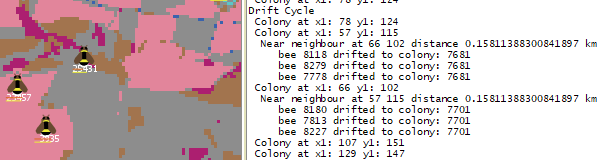
\includegraphics[scale=0.75]{img/mtd3/mtdp3v11-img001.png}
%     \caption{Migracijos įgyvendinimas jungtiniame modelyje}
%     \label{img:m1}
% \end{figure}


\subsubsection{Bičių mirtingumas pagal metų laiką}
Bumble-Beehave modelis taiko papildomą mirtingumo modelį motinėlėms žiemojimo metu pagal jos amžių ir masę, tačiau tokie skaičiavimai nėra taikomi darbininkėms, nes kamanių darbininkės nežiemoja.
Bičių darbininkės priklausomai nuo metų laiko ir darbų intensyvumo gyvena trumpiau ar ilgiau. Vasaros ir medunešio metu darbininkės išgyvena apie 6 savaites. Prieš žiemą užaugusios bitės, pasiruošusios žiemojimui, gali išgyventi ir iki 6 mėnesių. Bumble-Beehave modelis remiasi konstanta ir bitės miršta iškart pasiekusios maksimalų amžių pagal šią konstantą. Dabartinis sprendimo įgyvendinimas remiasi nurodytais \cite{YYY19} intervalais, dėl to darbininkės išgyvena žiemą.
Bumble-Beehave klimato modelį įgyvendina pagal valandas, per kurias bitė dienos metu gali ieškoti maisto. Pavyzdžiui, jeigu pasitaiko lietinga diena, tos valandos atimamos iš bendro laiko. Šį modelį vertėtų praplėsti identiškai pagal temperatūrą ir drėgmę, jog būtų nustatomas tikslesnis sunaudojamas energijos kiekis perų ir šeimos šildymui, tačiau tai nebuvo įgyvendinta šio darbo metu.
\subsection{Jungtinio modelio tikrinimas}
Sprendimas buvo kuriamas ir tikrinimas inkrementiniu būdu, pridedant naują bitininkystės procesą ir lyginant jį su buvusiais modeliais, juose irgi atitinkamai pakeitus modeliuojamos procesus.
Pateiktuose eksperimentuose nebuvo atsižvelgiama į tranų dauginimąsi, netikrinant tranų populiacijos motinėlių apvaisinimo metu. Tranai buvo nereikalingi tikrinant žiemojimo procesus, kadangi ir naminių bičių šeimose tranai yra išvaromi iš lizdo ir miršta rudenį, kaip ir kamanių šeimose. Papildomai nebuvo modeliuojamas motinėlių augimas, kadangi Bumble-Beehave modelis su visomis užaugusiomis motinėlėmis pavasarį bando įrengti naujas bičių šeimas, kas galioja kamanėms, tačiau naminėms bitėms galioja tik tuo atveju, jeigu pradinė šeima ruošiasi spiestis. Lyginant gautą sprendimą su Beehave modeliu nebuvo kuriamos naujos šeimos ar spietimosi procesai, kadangi Beehave modelis modeliuoja tik vieną šeimą. Šie procesai Bumble-Beehave modelyje vyksta jeigu modelyje atsiranda peržiemojusių motinėlių, taigi buvo sustabdytas motinėlių auginimas. Tai buvo atlikta Bumble-Beehave modelyje nurodant labai didelį svorį kiaušinėliams, lervoms ir  lėliukėms, jog šį išsivystytų į motinėlę. Taigi šiame etape naujų motinėlių atsiradimas nebuvo modeliuojamas.


\subsubsection{Lyginimas su Beehave modeliu}
Beehave populiacijos skaičiavimai buvo lyginami su empirinėmis žiniomis apie realią bičių šeimų populiacijos kaitą. Modelio trūkumai buvo nustatyti ir paviešinti Europos maisto saugos tarnybos \cite{EFSA15}. Esminiai trūkumai buvo pesticidų procesų trūkumas, primityvus landšafto (topografijos, augalijos) modelis, ribota klimato konfigūracija (modelis buvo pritaikytas centrinės Europos klimato zonai) ir apribotas ligų kiekis, tiriant tik varozę. Kadangi 	Bumble-Beehave modelis ištaisė klimato ir landšafto trūkumus, su idealiomis sąlygomis naujas modelis, atitinkantis empirines žinias, turėtų atitikti ir Beehave modelio gaunamus rezultatus.
Tikrinant kuriamą modelį buvo perkelti procesai iš Beehave modelio ir tikrinami parametrai ir daromi bandymai kol abiejų modelių gaunami bičių šeimų dydžiai, kiaušinėlių, sukaupto medaus ir žiedadulkių kiekiai pasidarė panašūs. Šie rezultatai buvo lyginamai pagal modelio kuriamų resursų grafikus (žr.~\ref{img:m2} ir~\ref{img:m3} pav.).



\begin{figure}[H]
    \centering
    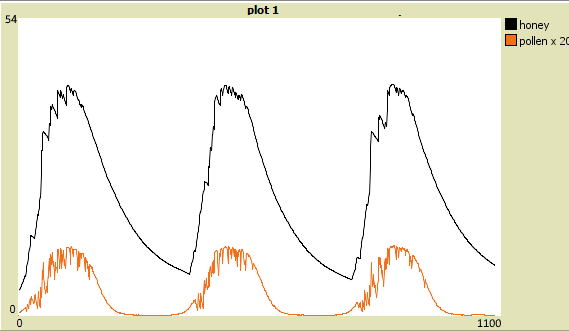
\includegraphics[scale=0.75]{img/mtd3/mtdp3v11-img002.png}
    \caption{Medaus kiekis (kg) ir žiedadulkių kiekis dabartiniame sprendime}
    \label{img:m2}
\end{figure}

\begin{figure}[H]
    \centering
    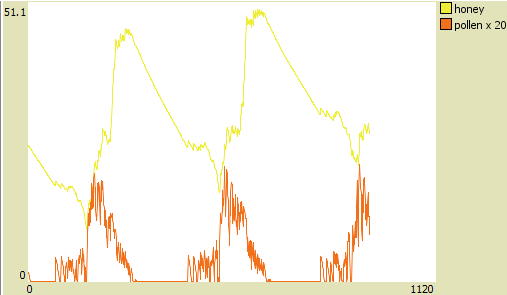
\includegraphics[scale=0.75]{img/mtd3/mtdp3v11-img003.png}
    \caption{Medaus kiekis (kg) ir žiedadulkių kiekis Beehave modelyje}
    \label{img:m3}
\end{figure}


	 Yra kiti skirtumai tarp modelių, kurie matosi nagrinėjant populiacijų ir sukaupto maisto (~\ref{img:m2} ir ~\ref{img:m3} pav.) skirtumus. Viena pagrindinių šio skirtumo priežasčių – maisto prieinamumas modeliuose. Beehave modelis turi tik du gėlių laukus, kurių nektaro ir žiedadulkių kiekis nurodomas normaliuoju skirstiniu (~\ref{img:m4} pav.), bet abu laukai turi skirtingus laikotarpius, kada bitės gali surinkti iš jų didžiausią kiekį maisto. Bumble-Beehave modelis gėlių ir augalų rūšis bei jų parametrus gauna pagal vieną iš įvesties failų, nurodančių skirtingų rūšių gėles ir augalus. Beehave modelyje bitės gali pasiekti abu gėlių laukus (~\ref{img:m5} pav.), tuo tarpu Bumble-Beehave modelyje atsižvelgiama į paties lauko atstumą nuo šeimos pagal pateikta žemėlapį (~\ref{img:m6} pav.) bei reikalingo bitės liežuvėlio ilgį, jog atskridusi bitė galėtų surinkti iš augalo nektarą.

\begin{figure}[H]
    \centering
    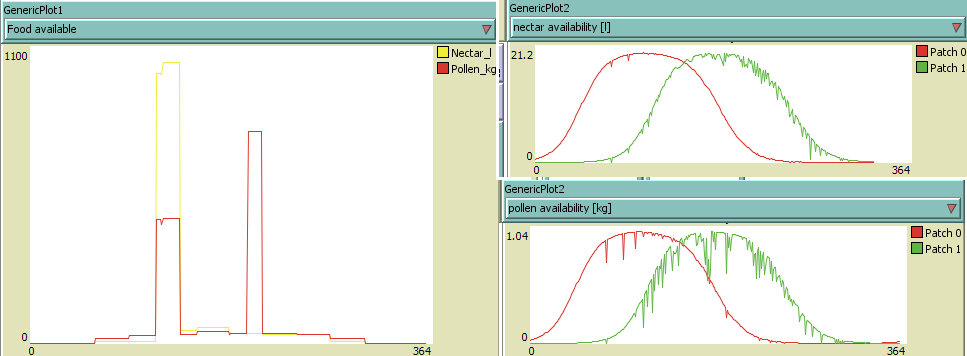
\includegraphics[scale=0.5]{img/mtd3/mtdp3v11-img004.png}
    \caption{Maisto pasiekiamumas naujajame modelyje (kairėje) ir Beehave (dešinėje)}
    \label{img:m4}
\end{figure}

\begin{figure}[H]
    \centering
    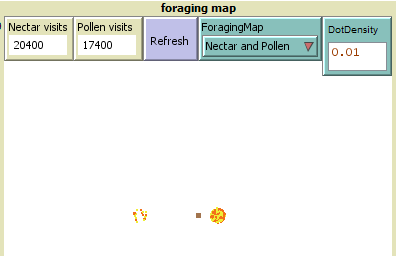
\includegraphics[scale=0.75]{img/mtd3/mtdp3v11-img005.png}
    \caption{Landšafto atvaizdavimas Beehave modelyje}
    \label{img:m5}
\end{figure}

\begin{figure}[H]
    \centering
    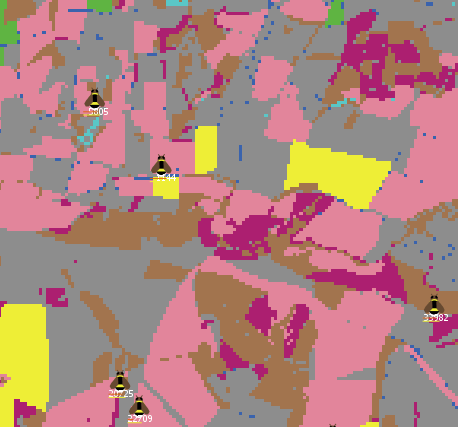
\includegraphics[scale=0.75]{img/mtd3/mtdp3v11-img006.png}
    \caption{Landšafto atvaizdavimas Bumble-Beehave modelyje}
    \label{img:m6}
\end{figure}




Šeimos sandara (~\ref{img:m7} ir~\ref{img:m8} pav.) išlieka panaši. Vasarą bičių šeima išauga iki 40-50 tūkstančių bičių, pavasarį sumažėja iki 6-4 tūkstančių.

\begin{figure}[H]
    \centering
    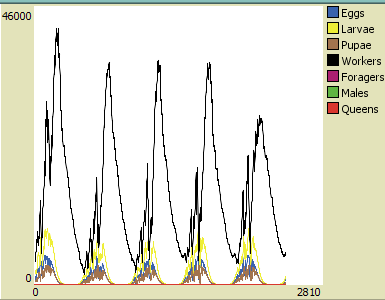
\includegraphics[scale=0.75]{img/mtd3/mtdp3v11-img007.png}
    \caption{Šeimos struktūra dabartiniame sprendime}
    \label{img:m7}
\end{figure}

\begin{figure}[H]
    \centering
    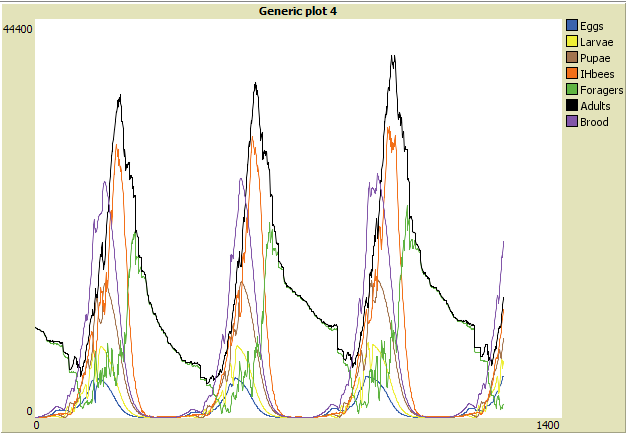
\includegraphics[scale=0.75]{img/mtd3/mtdp3v11-img008.png}
    \caption{Šeimos struktūra Beehave modelyje}
    \label{img:m8}
\end{figure}


Kiti skirtumai susiję su bičių mirtingumu. Dabartiniame sprendime atsižvelgiama tik į bičių mirtingumą paieškos metu ir jos didžiausią gyvenimo trukmę. Jog bitės galėtų peržiemoti, proporcingai buvo pakeista rudenį išsiritusių bičių gyvenimo trukmė, atitinkanti realius bičių šeimos procesus, kadangi žiemojančios bitės neieško maisto ir nenaudoja papildomų medžiagų nektaro vertimui į medų.  Beehave modelyje prie šio proceso prisideda ir bitės nukeliautas atstumas, kadangi bičių sparneliai nusidėvi intensyvaus darbo metu ir bitė miršta anksčiau, tačiau tai nesudaro didelio skirtumo, kadangi bitei ieškant maisto visais atvejais išauga tikimybė mirti.

\subsection{Jungtinio modelio aptarimas}


Darbo esminis sprendimas remiasi dvejais bitininkystės procesų modeliais, kurie turi daug esminių logikos skirtumų bei skirti modeliuoti skirtingą kiekį objektų ir skirtingoje aplinkoje. Tačiau kartu šie modeliai nusako didžiąją dalį procesų, kurie atspindi naminių bičių šeimos gyvenimą. Iš šiame skyriuje pateiktų grafikų matome, jog jungtiniame modelyje bičių populiacijos ir maisto kreivės yra panašios į BEEHAVE modelio kreives. Palyginkime gautus rezultatus su empirinėmis žiniomis.

Bičių šeimos išauga jeigu bitės gali rasti daug žiedadulkių. Tai labai priklauso nuo aplinkinės floros, kuri taip pat priklauso nuo vietovės. Pavyzdyje \cite{Oli15} teigiama, jog bičių šeimos dydis pasiekia viršūnę birželio ir liepos mėnesiais su 50 tūkstančių suaugusių bičių, o tarp lapkričio ir kovo laikosi ties 8 – 12 tūkstančių bičių riba. Tačiau populiacijos atžvilgiu panašius skaičius teikia ir lietuviški vadovėliai. Teigiama, jog stipri šeima užauga iki 60-65 tūkstančių darbininkių \cite{Kar00}. Šie rezultatai buvo pasiekiami ir dabartiniame sprendime, priklausomai nuo keičiamų landšafto duomenų. Tačiau šie vadovėliai nepateikia tikslios informacijos, tame pačiame šaltinyje stiprios šeimos nurodomos, turinčios 60-70 tūkstančių bičių vasarą ir 25-30 tūkstančių žiemojančių bičių, o tai viršija kitų šaltinių informaciją. 

Kitas nagrinėtas modelis, be nagrinėtų literatūros apžvalgos metu, teikia panašius rezultatus į Beehave bei remiasi HoPoMo modeliu \cite{ScC07,BWZ16}. Jame bičių šeimos kiekis sumažėja ir iki 4 tūkstančių bičių kiekio šeimoje, šis sumažėjimas įvyksta pavasario pradžioje, kai vėl dedami kiaušinėliai ir pirmosios bitės, ieškančios maisto, turi didžiausią mirtingumą. Vasarą pasiekia 40-50 tūkstančių bičių ribą.

Taigi, sukurtas jungtinis modelis modelis, veikiantis agentinio modeliavimo principu ir NetLogo paketu, atitinkantis empirines žinias ir BEEHAVE modelio gaunamus rezultatus. Trečiame skyriuje aptarsime naujus įgyvendintus procesus.

\begin{figure}[H]
    \centering
    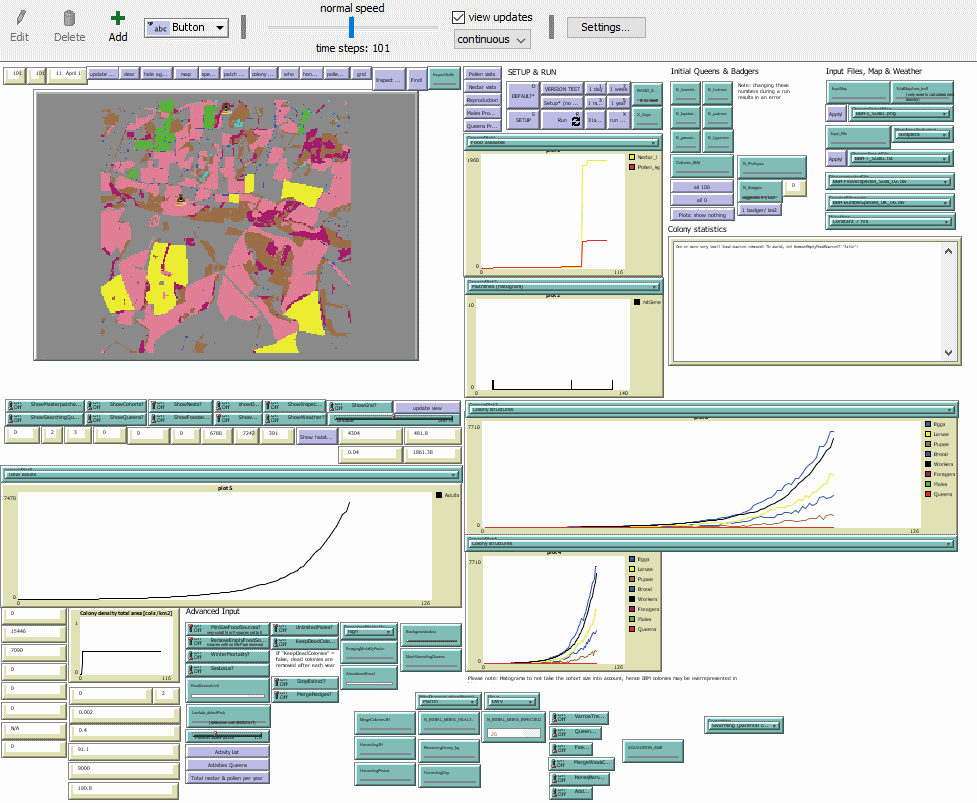
\includegraphics[scale=0.5]{img/new/gui.png}
    \caption{Grafinė jungtinio modelio grafinė sąsaja iš BEEHAVE ir Bumble-BEEHAVE elementų}
    \label{img:gui1}
\end{figure}



\section{Patobulintas modelis}

Praeitame skyriuje pristatytas jungtinis BEEHAVE ir Bumble-BEEHAVE modelis, bei procesai, kuriuos pavyko apjungti tarp modelių, jog būtų įmanoma modeliuoti kelias naminių bičių šeimas vienu metu. Dabar pabandykime praplėsti šį modelį naujais procesais. %todo bet// gavosi tik vienas?


% sudaro daugiau nei tre\v{c}dal\k{i} visų \v{s}eimos aktyvi\k{u} darbininki\k{u} skai\v{c}i\k{u}:


%Reikės gal perrašyti
\subsection{Bičių migracija tarp šeimų}
Jungtinį sprendimą papildykime bičių migracijos procesu, pagal kurį vėliau galėsime įgyvendinti ir bičių spietimąsi.

Literatūros analizės metu rasti empiriniai duomenis apie bičių migraciją \cite{PfC98, BPC16}, tačiau šiam procesui nebuvo pateiktas joks migracijos apskaičiavimo modelis. Galime remtis dar vienu straipsniu, pateikiančiu lygtį migruojančių bičių santykiui \cite{FNF15}:

\begin{equation}
    n_{steb\textit{\.{e}}tos} = 0,716 + \frac{13,96}{i_{kaimyno}}
\end{equation}



Kur $n_{steb\textit{\.{e}}tos}$ yra tyrime stebėtų migruojančių bičių kiekis į konkrečią stebimą šeimą iš kitų šeimų, esančių atstumu $i_{kaimyno}$. Nurodomo eksperimento metu 14 avilių buvo sustatyti 18 metrų ilgio eilėje, taigi $n_{kaimyno}$ beveik atitinka metrą, tačiau šį atstumą reiktų suprasti kaip pozicijos eilėje skirtumą arba indeksą. Jei $n_{kaimyno}=1$, tai reiškia, jog bitės į stebimą šeimą atkeliavo iš kairėje ir dešinėje esančių artimiausių kaimynų. Pateikti koeficientai atitinka tik eksperimente stebėtų bičių kiekį. Bendru atveju bitės imigrantės sudaro $17 ± 4\%$ bičių šeimos populiacijos \cite{BPC16}. 

Šie eksperimentai atlikti rudenį, tačiau pateikia panašius rezultatus kaip ir kiti stebėjimai \cite{PfC98, BPC16}, ir galima teigti, jog panašus migracijos pasiskirstymas vyksta ir vasaros metu. Taigi jungtiniame modelyje migracija įgyvendinama perskirstant bites, pasirinkus šeimą ir priskiriant kaimyninių šeimų bites pasirinktai šeimai. Atsižvelgiant į intensyviausio medaus nešimo laikus, kai dažniausiai pasitaiko migracijos reiškinys, mes galime pasirinktai bičių šeimai priskirti  imigruojančių bičių iš kiekvienos kaimynės kas 6 savaites, kadangi darbininkės tuo laikotarpiu tiek laiko ir gyvena. Tuo atveju pasiskaičiuojame pagal modelį sumą, kiek bičių $ n_{migruojan\textit{\v{c}}ios}$ migruotų pagal stebėjimą ir kaimynų didžiausią atstumą ${N_{kaimynai}}$.
\begin{equation}
    n_{migruojan\textit{\v{c}}ios} = \sum_{i=1}^{N_{kaimynai}} = 0,716 + \frac{13,96}{i}
\end{equation}
    Ir pagal duotą santykį 17\%±4\% santykį perskaičiuotame iš kiekvieno  $i_{kaimyno}$ atstumu esančio kaimyno gaunamą bičių kiekį $m_{migruojan\textit{\v{c}}ios}$ :
\begin{equation}   
    m_{migruojan\textit{\v{c}}ios} = (0,716 + \frac{13,96}{i_{kaimyno}}) \frac {0,22n_{visos}}{n_{migruojan\textit{\v{c}}ios}}
\end{equation}

Išbandykime šį migracijos kiekį su 20 bičių šeimų, kurių kiekvienos dydis po 1000 bičių (žr.~\ref{pavem} pav.). Mažiausias aptiktas bičių migrančių kiekis matomas pirmoje šeimoje ir sudaro 13,7\% visos bičių šeimos, tuo tarpu didžiausias migrančių kiekis matomas keturioliktoje šeimoje, kurioje migrantės sudaro 20,9\% visos šeimos populiacijos. Bičių migrančių pasiskirstymas atitinka šaltinyje nurodomus intervalus.

\begin{figure}[H]
    \centering
    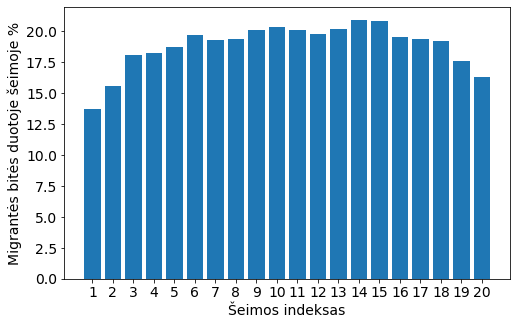
\includegraphics[scale=0.7]{img/new/emi.png}
    \caption{Bičių migrančių pasiskirstymas. Šeimos indeksų skirtumus galime laikyti $i_{kaimyno}$ indeksu}
    \label{pavem}
\end{figure}


Taigi, jungtinį modelį galima būtų praplėsti bičių migracijos procesu, tačiau jis galioja tik labai ribotomis sąlygomis. Tyrimo metu nebuvo pritaikyti varozės plitimo procesai tarp šeimų, o šiame procese ir pateikto straipsnio \cite{BPC16} modelyje pateikiamas idealizuotas atvejis, jei bitės migruoja nepaveiktos ligų. Be to, šis procesas galioja tik jei atstumas tarp bičių šeimų yra labai mažas ir atitinka bityną. Be to, aptariamas modelis remiasi eksperimentu, atliktu su bičių migraciją skatinančiomis sąlygomis: aviliai buvo nudažyti identiškai, avilių lakos (pro kur bitė įskrenda į avilį), buvo nukreiptos į tą pačią pusę. Taigi, nors pristatytas migracijos procesas remiasi empiriniais duomenimis, jį būtų verta perdaryti prijungus varozės procesus.


\subsection{Spietimosi procesas ir algoritmas}

 Įprastai rastą maisto šaltinį bitės nurodo kitoms bitėms šokio metu, o priklausomai nuo maisto šaltinio kokybės, šis šokis vyksta trumpiau arba ilgiau, jog šokį stebinčios bitės turėtų daugiau progų pasirinkti geresnį šaltinį ilgesnio šokio metu. 
 
 Kai spiečiasi bitės, šeima susispiečia į kamuolį aplink motinėlę, o apie 300-500 bičių žvalgų atlieka naujo būsto paiešką. Tačiau suradusios naują lizdą ir iš naujo šokdamos ir tikrindamos rastą vietą, šios bitės kiekvieną kartą, nepaisant nepakitusios lizdo kokybės, trumpina savo šokio ilgį. Pagal stebėjimus nurodoma, jog geros kokybės lizdą apibūdinantis šokis trunka apie šimtą ciklų ir su kiekvienu pakartotiniu patikrinimu sumažinamas 10-15 ciklų \cite{See10}. Taigi, geros kokybės lizdai po kelių pakartotinių apsilankymų nusakomi tarsi turėtų mažesnę kokybę. Toks geriausio lizdo atsisakymas leidžia stebėtojoms pasirinkti kitus lizdus dažniau ir išbandyti daugiau variantų. 
 
 Šį slopinimo reiškinį verta ištirti plačiau. Toliau aptarsime dirbtinės bičių šeimos algoritmus, kurie remiasi maisto šaltinio paieška, bei pabandysime šiuos algoritmus pritaikyti spietimosi procesui.


\subsubsection{Dirbtinės bičių šeimos algoritmas}



%Dar reikia pataisyti intro ABC
Dirbtinės bičių šeimos algoritmas \cite{KaB07} priklauso kolektyvinio intelekto algoritmų šeimai ir yra metaeuristinių optimizavimo metodų pogrupis \cite{MBB11}.
Šie algoritmai skirti spręsti sudėtingus optimizavimo uždavinius, kurie turi daug optimizavimo kriterijų.
Optimizavimo uždavinius galime apibrėžti pora $(S, f)$; čia $S$ žymi sprendinių aibę, o $f$ – skaliarinę tikslo funkciją, kurios apibrėžimo sritis – $S$, o reikšmių aibė – realieji skaičiai. Tuomet išspręsti uždavinį $(S, f)$ reiškia surasti sprendinį $s$:

\begin{equation}\label{sol}
s \in  S = \{s^{\nabla} | s^{\nabla} = argmin_{s \in S} f(s)\}.
\end{equation}

Čia $s$ yra globaliai optimalaus sprendinys. Ieškosime sprendinio, kuriame tikslo funkcija įgyja minimalią reikšmę, t.y. minimizuojama. Panagrinėkime kelias klasikines tikslo funkcijas, naudojamas metaeuristinių algoritmų efektyvumo lyginimui.~\ref{tab:classic}-oje lentelėje nurodomos darbe naudojamos klasikinės fukcijos ir jų tipai. M - funkcija multimodalinė, turinti daugiau nei vieną modą (nors šiame kontekste laikoma, kad turi vieną minimumą), U - unimodalinė, S - atskiriama (duotai funkcijai $h(x,y)$ galioja $h(x,y)=h_{1}(x)h_{2}(y)$), N - neatskiriama. Verta paminėti, jog Schwefel funkcija \cite{Sch81}, pateikta \cite{ABK19} šaltinyje ir naudojama šiame darbe, įprastai apibrėžiama $f(x_{1}\dots x_{n}) = \sum_{i=1}^{D} (-x_{i}\sin{(\sqrt{|x_{i}|})}) + 418,982887 * D$ ir jos minimumas lygus 0, tačiau bus naudojamas variantas, nurodytas ~\ref{tab:classic}-oje lentelėje. Šios funkcijos ir jų testavimas implementuotas Python kalba. 


\begin{table}
\centering
\caption{Klasikinės tikslo funkcijos optimizavimo uždaviniams}
\label{tab:classic}
\begin{tabular}{p{0.12\linewidth}|p{0.03\linewidth}|p{0.05\linewidth}|p{0.14\linewidth}|p{0.15\linewidth}|p{0.4\linewidth}}
Funk\-ci\-ja&Ti\-pas&Di\-men\-si\-ja $(D)$&Spren\-di\-nių ai\-bė&Mi\-ni\-mu\-mas&For\-mu\-lė \\
\hline
Sferos & US & $30$ & $[-100,100]^{D}$ & 0 &$f(x)=\sum_{i=1}^{D} (x_{i}^{2})$ \\
\hline
Rosenbrock & UN & $30$ & $[-30,30]^{D}$ & 0 &$f(x)=\sum_{i=1}^{D} (100(x_{i+1}-x_{i})^{2}+(x_{i}-1)^{2})$ \\
\hline
Rastrigin & MS & $30$ & $[-5.12,5.12]^{D}$ & 0 &$f(x)=\sum_{i=1}^{D} (x_{i}^{2}-10\cos{2\pi x_{i}}+10)$ \\
\hline
Dixon Price & UN & $30$ & $[-10,10]^{D}$ & 0 &$f(x)= (x_{1})-1)^{2} \sum_{i=2}^{D} (i(2x_{i}^{2}-x_{i-1})^{2})$ \\
\hline
Ackley & MN & $30$ & $[-32,32]^{D}$ & 0 &$f(x)=20+e-20\exp{(-0.2\sqrt{\frac{1}{D}}\sum_{i=1}^{D} (x_{i}^{2}))} - \exp{\frac{1}{D}\sum_{i=1}^{D} \cos{2\pi x_{i}}}$ \\
\hline
Schwefel & MS & $30$ & $[-500,500]^{D}$ & -125\-69,5 &$f(x)=\sum_{i=1}^{D} (-x_{i}\sin{(\sqrt{|x_{i}|})})$ \\
\hline
Griewank & MN & $30$ & $[-600,600]^{D}$ & 0 &$f(x)=\frac{1}{4000}(\sum_{i=1}^{D} (x_{i}^{2})) - (\prod_{i=1}^{D}\cos{(\frac{x_{i}}{\sqrt{i}})})+1$ \\
\hline
Kupra\-nugario (camel) & MN & $2$ & $[-5,5]^{D}$ & -1,03163 &$f(x)=4x_{1}^{2}-2,1x_{1}^{4}+\frac{1}{3}x^{6}_{1}+x_{1}x{2}-4x^{2}_{2}+4x^{4}_{2}$ \\
\hline
Branin & MN & $2$ & $[-5,10]^{D}$ & 0,39789 &$f(x)=(x_{2}+5-\frac{5,1}{4\pi^{2}}-6)^{2}+10(1-\frac{1}{8\pi})\cos{x_{1}}+10$
\end{tabular}
\end{table}


Dirbtinį bičių šeimos algoritmą galime aprašyti šiais žingsniais:

\begin{enumerate}
    \item	Inicializacija. Nustatomi algoritmo parametrai. Spiečiaus populiacijos dydis, algoritmo ciklų vykdymo kiekis, algoritmo baigimo kriterijai. Visos populiacijos individualioms bitėms pritaikomas atsitiktinis sprendinys sprendinių aibės ribose $[k,j]$:

\begin{equation}\label{ei1}
x_{m,i}=k_{i}+rand(0,1)(j_{i}-k_{i})
\end{equation}


    \item 	Bičių darbininkių fazė. Kiekvienas sprendinys gerinamas pagal nustatytą lokaliojo gerinimo procedūrą, ir, radus geresnį sprendinį, dabartinis bitės sprendinys pakeičiamas geresniu. Naujas sprendinys $v_{m,\ i}$   ieškomas keičiant $x_{m,\ i}$:

\begin{equation}\label{eebp1}
v_{m,\ i}=x_{m,\ i} +\phi_{m,\ i} (x_{m,\ i} -x_{k,i} )
\end{equation}

Čia $\phi_{m,i}$ atsitiktinis skaičius tarp [-1,1]. Bitės rinkėjos atliktų šį vaidmenį realioje šeimoje.

    \item 	Stebinčių bičių fazė. Praeitame žingsnyje rasti ir gerinami bičių sprendiniai perduodami kitoms bitėms, apskaičiuojant tikimybes kiekvienam sprendiniui, jog stebinčioji bitė pasirinks gerinti tą sprendinį. Ši tikimybė proporcinga skaičiuojamo sprendinio kokybei pagal tinkamumo funkcijos reikšmę:

\begin{equation}
\label{eobp1}
p_m=\frac{fit(x_m)}{\sum_{m=1}^{CS}{fit(x_m)}}
\end{equation}
Kur $CS$ yra šeimos dydis, o tinkamumo funkcija $fit(x_m)$ apskaičiuojama pagal tikslo funkciją $f(x)$:
\l \begin{equation}\label{efit}
fit(x_m)=
\begin{cases}
1+f(x_m), jei f(x_m)>0\\
\frac{1}{1+|f(x_m)|}, jei f(x_m)\leq0
\end{cases}
\end{equation}


    \item 	Bičių žvalgų fazė. Jei konkretus sprendinys antroje fazėje buvo nesėkmingai gerintas nustatytą kiekį kartų $l$, jis yra atmetamas ir pakeičiamas kitu atsitiktinai parenkamu sprendiniu pagal \eqref{ei1}. Bitės lankuolės atliktų šio ir stebinčių bičių žingsnių vaidmenius realioje bičių šeimoje.

    \item 	Įsimenamas geriausias rezultatas. Jeigu rezultatas netenkina baigimo sąlygų, grįžtama į antrą žingsnį. Baigimo salygos įprastai yra algoritmų iteracijų riba, tačiau dėl algoritmo lyginimo tikslų arba dėl ribotų resursų, šie kriterijai taip pat gali būti tikslo funkcijos skaičiavimų kiekis arba bendras vykdymo laikas. Paprastoje šio algoritmo versijoje tai yra iteracijų kiekis, kuris šiame žingsnyje didinamas vienetu.

\end{enumerate}



Šis algoritmas turi įvairius galimus pakeitimus, gerinančius jo našumą. Vienas taikomų metodų inicializacijos žingsnyje pritaikyti papildomas sprendinių lokaliojo pagerinimo ar išbarstymo procedūras. Aptarkime keletą tokių algoritmo pakeitimų.



Pradiniame Karabogos algoritme \cite{KaB07}  bitės stebėtojos pasirinkdavo naują sprendinį pagal tą patį algoritmą kaip ir dirbančios bitės. Realybėje stebinčios bitės ieškotų naujo maisto šaltinio dirbančios bitės nurodytos vietos kaimynystėje. Tuo pagrindu sukurtas greitasis dirbtinės bičių kolonijos algoritmas \cite{KaG14} (angl. Quick Artificial Bee Colony algorithm arba qABC), kuris remiasi naujo sprendinio ieškojimu pagal pasirinkto sprendinio kaimynystėje esančiais sprendiniais. Kaimynystė šaltinyje pateikiama kaip euklidinis atstumas tarp sprendinių: 

\begin{equation}
\label{eqabcbest}
v_{N_m,\ i}^{geriausias}=x_{N_m,\ i}^{geriausias}+\phi_{m,\ i}^{geriausias}(x_{N_m,\ i}^{geriausias}-x_{k,i} )
\end{equation}

Verta pastebėti, jog naujasis sprendinys remiasi geriausio kaimyno sprendinio vektoriumi, o ne buvusio sprendinio vektoriumi kaip paprastame dirbtinės bičių šeimos algoritme.


Šio algoritmo pagrindu sukurtas dar kitas jo patobulinimas, vadinamas patobulintu greituoju dirbtinės bičių šeimos algoritmu (angl. Improved Quick Artificial Bee Colony algorithm arba iqABC) \cite{ABK19}.
Patobulintas greitasis dirbtinės bičių šeimos algoritmas panašią formulę \eqref{eqabcbest} pritaiko ir stebėtojoms\eqref{eiqabcobp}, ir darbininkėms\eqref{eiqabcebp}:

\begin{equation}\label{eiqabcobp}
v_{N_m,\ i}^{isimintas}=x_{N_m,\ i}^{isimintas}+\phi_{m,\ i}^{isimintas}(x_{N_m,\ i}^{geriausias}-x_{k,i} )
\end{equation}

\begin{equation}\label{eiqabcebp}
v_{N_m,\ i}^{isimintas}=x_{N_m,\ i}^{isimintas}+\phi_{m,\ i}^{isimintas}(x_{N_m,\ i}^{geriausias}-x_{j,i} )
\end{equation}


Tačiau čia $x_{N_{m,i}}^{isimintas}$ yra ne $x_{k,i}$  kaimynas, o geriausias įsimintas sprendinys. Jis tikrinamas $l_{darbininkiu}$ kiekį kartų darbininkių žingsnyje ir tiek pat kartų $l_{stebinciu}$ tikrinamas stebinčiųjų bičių žingsnyje. Bendrai vadinkime šią ribą $l_{geriausias}$. Viršijus šią ribą, $l_{geriausias}$ riba pakeičiama į $l$ ribą atitinkamam žingsniui, kartu pakeičiant naudojamas formules į paprasto bičių šeimos algoritmo formules \eqref{eebp1} \eqref{eobp1}. 

Taigi iqABC algoritmas turi keturis režimus:
\begin{itemize}
    \item Kai darbininkių žingsniui taikoma \eqref{eiqabcobp} ir stebėtojų žingsniui \eqref{eiqabcebp}.
    \item Kai darbininkių žingsniui taikoma ABC formulė \eqref{eebp1}, o stebėtojų žingsniui \eqref{eiqabcebp}.
    \item Kai darbininkių žingsniui taikoma \eqref{eiqabcebp}, o stebėtojų žingsniui ABC formulė \eqref{eobp1}.
    \item Kai algoritmas veikia pagal ABC formules \eqref{eebp1}  \eqref{eobp1}
\end{itemize}

Šis algoritmas su kiekvienu tikslo funkcijos įvertinimu greičiau konverguoja link globalaus minimumo, nei įprastas ABC arba qABC. Kadangi daugiau sprendinių ieškoma aplink geriausią pradinį žinomą sprendinį, jei pradinėje sprendinių aibėje pasitaikė geras sprendinys, šis algoritmas konverguoja žymiai greičiau.

Dirbtinis bičių šeimos algoritmas remiasi bičių maisto paieškos procesais realiame pasaulyje. Tačiau iš atliktų stebėjimų matome, jog bičių elgesys maisto paieškos ir naujo lizdo paieškos metu skiriasi. Besispiesdamos bitės stengiasi kaip galima greičiau rasti geriausią naujo lizdo vietą. Toliau aptarsime spietimosi principus.


\subsubsection{Dirbtinio spietimosi algoritmas}

Poskyrio pradžioje minėjome spietimosi procese pastebimą slopinimo reiškinį. Dirbtinių bičių šeimų algoritmai slopinimą įgyvendina tik dalinai, turi šaltinio tikrinimo ribas, tačiau pačios ribos tėra konstantos.

Atsižvelgiant į pagreitintus dirbinių bičių algoritmus galime pakeisti vieno sprendinio tikrinimo ribą pagal jo tikslo funkcijos reikšmę, o ne pagal konstantą. Vienintelis iššūkis šio principo pritaikyme – mes iš anksto nežinome geriausios tikslo funkcijos reikšmės iš anksto vykdydami algoritmą. Šiuo atveju santykinį sprendinio tinkamumą vertinsime pagal didžiausią ir mažiausią žinomą tikslo funkcijos reikšmę. Šį principą išbandysime taikydami jį patobulinto greitojo bičių algoritmo žingsniams (iqABC).

Patobulinto greitojo bičių algoritmo atžvilgiu keisime stebinčių bičių žingsnio tikimybės formulę ir visas tikrinimo ribas. Stebinčių bičių žingsnyje sprendinio tikrinimo tikimybės  $p_{m}$ formulė \eqref{iqsobp} atsižvelgs į sprendinio prieš tai buvusių bandymų kiekį\eqref{iqsobp2}:

\begin{equation}\label{iqsobp}
p_{m, santykinis}=\frac{g(x_m)}{\sum_{m=1}^{CS}{g(x_m)}}
\end{equation}

\begin{equation}\label{iqsobp2}
g(x_m)=\frac{fit(x_{m})}{norm(x_{m})}bandymai(x_{m})
\end{equation}
Kur $norm(x_{m})$ funkcija priskiria $2$ mažiausiai rastai reikšmei ir $1$ didžiausiai rastai reikšmei, kadangi bandome minimizuoti tikslo funkciją:
\begin{equation}\label{iqsobp3}
        norm(x_{m}) = 1 + \frac{fit(x_{blogiausias})-fit(x_{m})}{fit(x_{blogiausias})-fit(x_{geriausias})}
\end{equation}

Bendrą iqABC ribą $l_{geriausias}$ keičiame į naują ribą $l_{santykinis}(x)$, kuri nėra konstanta, o apskaičiuojama pagal geriausio ir prasčiausio rasto sprendinio santykį \eqref{iqslim1}. Viršijus šią ribą, $l_{santykinis}(x)$ pakeičiamas į $l_{naujas}(x)$ ribą atitinkamam žingsniui, kartu pakeičiant naudojamas formules į paprasto bičių šeimos algoritmo formules \eqref{eebp1} \eqref{eobp1}, tačiau $l_{naujas}(x)$, palyginus su ABC ketvirto žingsnio $l$ riba, taip pat perskaičiuojamas pagal geriausią ir prasčiausią sprendinį. 

\begin{equation}\label{iqslim1}
        l_{geriausias}(x)=bandymai(x_{m})norm(x_{m})l_{geriausias}
\end{equation}

\begin{equation}\label{iqslim2}
        l_{naujas}(x)=bandymai(x_{m})norm(x_{m})l
\end{equation}

Ciklo pabaigoje be geriausio sprendinio  $x_{geriausias}$ įsimenamas ir blogiausias $x_{blogiausias}$ sprendinys.





Bičių žvalgų ir dirbančiųjų žingsnyje jei konkretus sprendinys $(x_m)$ buvo nesėkmingai gerintas $k(x_m)$ kartų , jis yra atmetamas ir pakeičiamas kitu atsitiktinai parenkamu sprendiniu:

\begin{equation}\label{iqssp}
k(x_m) = fit(x_{geriausias})norm(x_{m}){bandymai(x_m)}
\end{equation}


Algoritmą, veikiantį su šiais pakeitimais, pavadinkime patobulintu greituoju besispiečiančios šeimos algoritmu (angl. Improved Quick Swarming Artificial Bee Colony arba iqsABC). Šio algoritmo bičių žvalgų ir darbininkių žingsnių pseudokodas pateikiamas 5 priede.
Šis algoritmas buvo įgyvendintas su Python programavimo kalba, besiremiant įprasto ABC algoritmo implementacija HIVE \cite{Wui17}, tačiau ją pakeitus, jog būtų kaupiama informacija pagal kiekvieną tikslo funkcijos įvertinimą ir algoritmas būtų baigiamas pasiekus nustatytą tikslo funkcijos tikrinimų ribą. Tuo pačiu principu įgyvendinti ir iqABC bei qABC algoritmai, kurie bus naudojami kitame skyriuje.

\subsubsection{Dirbtinių bičių šeimų algoritmų lyginimas}


Dirbtinių bičių šeimų algoritmai nėra determinuoti ir turi daug versijų, taigi šių algoritmų lyginimui yra nurodyti principai, kurių rekomenduojama laikytis \cite{MLK15}, nustatant šių algoritmų efektyvumą

Dirbtinių bičių šeimų algoritmų lyginimui reikia nubrėžti:
\begin{itemize}
    \item Ribotą tikslo funkcijos įvertinimų kiekį
    \item Rezultatų konvergavimo diagramas su vienodu funkcijos įvertinimo kiekiu
\end{itemize}

Dirbtinių bičių šeimos algoritmo sudėtingumas pagal pateiktas rekomendacijas skaičiuojamas pagal tikslo funkcijos įvertinimo kiekį. Paprastojo bičių šeimos algoritmo šaltinyje pateikiama, jog to algoritmo sudėtingumas yra $2\times CS\times L$, kur $CS$ bičių kiekis naudojamas du kartus dėl bičių darbininkių ir stebėtojų žingsnio, o $L$ yra iteracijų riba. Papildomai inicializacijos žingsnyje sukuriant pradinius sprendinius atliekamas $CS$ kiekis tikslo funkcijos įvertinimų. Tobulinant algoritmus kartais pasitelkiama daugiau tikslo funkcijos įvertinimų, tačiau atsižvelgiama tik į bendrą iteracijų kiekį. Taigi kai kurie algoritmai, nors ir daugiau kartų skaičiuoja tikslo funkciją, šaltiniuose pristatomi tarsi turėtų tą patį sudėtingumą. Kuriant naująjį spietimosi algoritmą buvo padaryta ta pati klaida, kadangi darbininkių fazėje naujas rastas sprendinys \eqref{eebp1} gali būti atmestas ir perskaičiuotas žvalgų fazėje \eqref{ei1}, o tai naudoja papildomą tikslo funkcijos skaičiavimą. Todėl būtina algoritmo baigimo kriterijų iš iteracijų ribos pakeisti į tikslo funkcijos įvertinimų kiekį. Toliau pateikiami rezultatai remsis tikslo funkcijų įvertinimų riba.


Atsižvelgiant į prieš tai pateiktus algoritmus \cite{ABK19, KaG14}, prasminga nustatyti panašias sprendinio tikrinimo ir kitų parametrų vertes , kurias pateikia kiti šaltiniai (žr.~\ref{tab:par} lentelę). 




\begin{table}[H]
\centering
\caption{iqsABC algoritmo vertinime naudojamos parametrų reikšmės klasikinėms funkcijoms}
\label{tab:par}
\begin{tabular}{llXl}
Kintamasis&Prasmė&Perimtas iš algoritmo&Reikšmė \\
\hline
$CS$ & Bičių šeimos dydis (pradinių sprendinių kiekis) & ABC & 50 \\ \hline
$D$& Dimensijos (kintamųjų kiekis) & ABC & $30$ \\ \hline
$l$ & Sprendinio tikrinimo riba & ABC & $\frac{CS\times D}{2}$ \\ \hline
$l_{geriausias}$ & Sprendinio tikrinimo riba geriausiam sprendiniui & iqABC & $CS \times D$\\ \hline
-& Tikslo funkcijų vertinimo riba & - & 500000\\ \hline
-& Bandymų kiekis & - & $30$

\end{tabular}
\end{table}

Pasirinkus atitinkančius parametrus ABC, qABC, iqABC ir iqsABC algoritmai buvo išbandyti su klasikinėmis tikslo funkcijomis (žr.~\ref{tab:classic} lentelę)  bei jų gaunami rezultatai ir konvergavimo grafikai palyginti su prieš tai buvusių algoritmų šaltiniais (šie grafikai pateikiami 3 priede).

Plačiau analizuosime skirtumus tarp iqABC algoritmo ir pagal jį sukurto naujo iqsABC algoritmo.

%Papildyti


Kadangi analizuojami algoritmai yra nedeterminuoti, gautų rezultatų tikrinimas nesuteikia prasmingo algoritmo įvertinimo. Rezultatų skirtumui įvertinti pasitelkiamas Wilcoxon testas \cite{Wil45}, skirtas įrodyti statistinėms hipotezėms \eqref{wilcoxon} duomenims, kai neturime išankstinių prielaidų apie duomenis. Hipotezę $H_{0}$ atmesime tik tuo atveju, jei testo duodama reikšmė $p<0.05$. %pirmo rasto šaltinio aprašymas, gal tiks pakeitimas%

%http://www.statistika.mif.vu.lt/wp-content/uploads/2014/05/Ivadas-i-statistika-su-R-2012xi30_t.pdf
%http://www.statistika.mif.vu.lt/wp-content/uploads/2014/04/SPSS_konspektai_2015.pdf


\begin{equation}\label{wilcoxon}
\begin{matrix}
H_{0}: skirstinys1 = skirstinys2 \\
H_{1}: skristinys1 \neq skirstinys2
\end{matrix}
\end{equation}


%tik aiškinant tada reiktų apskaičiuoti ir pavaizduoti Wilcoxon skirstinį ir nebežinau ar verta aprašinėti

Wilcoxon testas atliekamas su $2N$ reikšmių tarp 2 skirtingų vienodo dydžio imčių. Randame skirtumą tarp kiekvienos poros reikšmių, įsimename ženklą ir atmetame reikšmių poras, kurių skirtumas lygus 0. Likusias reikšmes žymime $N_{r}$. Išrikiuojame skirtumus nuo mažiausio iki didžiausio ir priskiriame numerį $R$ pagal eilės tvarką, pradedant nuo vieneto. Suskaičiuojame testo statistiką $W$ pagal formulę\eqref{eq:wil2}:
\begin{equation}\label{eq:wil1}
    W = \sum^{N_{r}}_{i=1} [sgn(x_{2,1}-x_{1,1}] R_{i}
\end{equation}
Tuo atveju, jeigu hipotezė $H_{0}$ teisinga, W reikšmės patenka į savą skirstinį. Jei $N_{r} \geq 20$,  standartinis įvertis $z$ apskaičiuojamas pagal formulę\eqref{eq:wil2}:
\begin{equation}\label{eq:wil2}
    z = \frac{W}{\sqrt{\frac{N_{r}(N_{r}+1)(2N_{r}+1)}{6}}}
\end{equation}
$H_{0}$ atmetama, jei $z_{kritinis} < |z|$, kur  $z_{kritinis}$ yra kritinė $W$ skirstinio reikšmė. Pagal tą patį skirstinį skaičiuojamos ir p-reikšmės.



Bandymai buvo atliekami dvejais aspektais:
\begin{itemize}
    \item Algoritmo veikimas rezultatų konvergavimo atžvilgiu. Kiekvieno bandymo metu atliekami tik 2000 tikslo funkcijos įvertinimų. Iš šių rezultatų po kiekvieno funkcijos įvertinimo gauto geriausio rezultato brėžiami konvergavimo grafikai.
    \item Algoritmo veikimas ilgalaikio tikslumo atžvilgiu. Kiekvieno bandymo metu atliekami 500000 tikslo funkcijos įvertinimų. Konvergavimo grafikai nebuvo sudaryti dėl labai mažų geriausių rastų reikšmių ir jų skirtumo artėjant prie algoritmo užbaigimo kriterijaus.
\end{itemize}

Analizuojant algoritmų rezultatus su klasikinėmis tikslo funkcijomis nepastebėti reikšmingi konvergavimo ar gaunamų rezultatų skirtumai. Rezultatų vidurkių skirtumus ir Wilcoxon testo rezultatus jiems matome~\ref{tab:s500kc} ir~\ref{tab:2kc} lentelėje. Konvergavimo diagramos pateikiamos 1 priede. Su 500000 tikslo funkcijos vertinimų iqabc geriau pasirodė su Griewank funkcija, tačiau su mažesniu nei $10^{-16}$ skirtumu. Su 2500 tikslo funkcijos vertinimų iqsABC geriau pasirodė su Branin, Dixon ir Schaffer funkcijomis, tuo tarpu iqABC geresnius rezultatus davė Schwefel funkcijai.


\begin{table}[H]
\centering
\small
\caption{iqsABC algoritmo efektyvumas su klasikinėmis tikslo funkcijomis kai $D=30$ (500000 tikslo funkcijos skaičiavimų)}
\label{tab:s500kc}
\begin{tabular}{l|l| n{8}{3}| n{8}{4}}
% Tikslo funkcija & \makecell{Statistiškai geresnis \\ algoritmas} & \makecell{Atsakymo vidurkio \\ skirtumas ABC-sABC} & p reikšmė \\
 Tikslo funkcija & Statistiškai geresnis & \text{Atsakymo vidurkio} & \text{p reikšmė} \\
  & algoritmas &   \text{skirtumas ABC-sABC} & \\
Ackley&-&-0.000000&0.052\\
Branin&-&-0&1.000\\
Camel&-&0.000000&0.480\\
Dixon&-&0.689147&0.382\\
Griewank&iqabc&-0.000000&0.020\\
Rastrigin&-&0&1.0000\\
Rosenbrock&-&0.001196&0.417\\
Schaffer&-&-0.000000&0.926\\
Schwefel&-&0.000000&1.000\\
Sphere&-&0.000000&0.750\\

% Ackley&-&-0.000000&0.0519\\
% Branin&-&-0&1.0000\\
% Camel&-&0.000000&0.4795\\
% Dixon&-&0.689147&0.3820\\
% Griewank&iqabc&-0.000000&0.0196\\
% Rastrigin&-&0&1.0000\\
% Rosenbrock&-&0.001196&0.4165\\
% Schaffer&-&-0.000000&0.9263\\
% Schwefel&-&0.000000&1.0000\\
% Sphere&-&0.000000&0.7499\\
\end{tabular}
\end{table}


%paskutinis rezultatas
\begin{table}[H]
\centering
\small
\caption{iqsABC algoritmo efektyvumas su klasikinėmis funkcijomis kai $D=30$ (2500 tikslo funkcijos skaičiavimų)}
\label{tab:2kc}
\begin{tabular}{l|l| n{8}{3}| n{8}{3}}
% Tikslo funkcija & \makecell{Statistiškai geresnis \\ algoritmas} & \makecell{Atsakymo vidurkio \\ skirtumas ABC-sABC} & p reikšmė \\
 Tikslo funkcija & Statistiškai geresnis & \text{Atsakymo vidurkio} & \text{p reikšmė} \\
  & algoritmas &   \text{skirtumas ABC-sABC} & \\
\hline
Ackley&-&0.039341&0.894\\
Branin&iqsabc&0.000004&0.035\\
Camel&-&-0.000000&0.797\\
Dixon&iqsabc&394271.844461&0.030\\
Griewank&-&-0.002681&0.644\\
Rastrigin&-&-0.414406&0.185\\
Rosenbrock&-&-0.963613&0.797\\
Schaffer&iqsabc&0.000326&0.035\\
Schwefel&iqabc&-1188.677962&0.000\\
Sphere&-&-1.239227&0.910\\
% Ackley&-&0.039341&0.8936\\
% Branin&iqsabc&0.000004&0.0350\\
% Camel&-&-0.000000&0.7971\\
% Dixon&iqsabc&394271.844461&0.0300\\
% Griewank&-&-0.002681&0.6435\\
% Rastrigin&-&-0.414406&0.1846\\
% Rosenbrock&-&-0.963613&0.7971\\
% Schaffer&iqsabc&0.000326&0.0350\\
% Schwefel&iqabc&-1188.677962&0.0000\\
% Sphere&-&-1.239227&0.9099\\
\end{tabular}
\end{table}





Išsamesnei analizei pasitelktos papildomos tikslo funkcijos \cite{CLZ14} (žr.~\ref{tab:extra}. lentelę). Funkcijos nuo $f_{10}$ iki $f_{15}$ yra sudėtinės, t.y. $F(x)=f(z_{1})+...+f(z_{n})$, kur $n$ yra sudedamųjų funkcijų kiekis, o $z$ yra kintamųjų $x$ poaibis, kur $x$ kintamieji paslinkti, jog sprendinių ieškojimas vyktų intervale $[-100,100]^{D}$, o globalų minimumą duodantys kintamieji būtų intervale $[-80,80]^{D}$. Šis paslinkimas naudojamas ir likusioms funkcijoms. Šių funkcijų pritaikymui naudota pateikto šaltinio \cite{CLZ14} funkcijų implementacija C kalba, į kurią realizuoti dirbtinių bičių šeimų algoritmai kreipėsi per Python ctypes biblioteką.

\begin{table}[H]
\centering
\caption{Papildomos tikslo funkcijos optimizavimo uždaviniams}
\label{tab:extra}
\begin{tabular}{r|l|r|l}
Nr.&Funk\-ci\-ja&Nr.&Funk\-ci\-ja\\
\hline
$f_{1}$ & Lenkto cigaro   &$f_{9}$ & Schaffer $f_6$\\
$f_{2}$ & Disko           &$f_{10}$ & Elipsės su $f_8$\\
$f_{3}$ & Weierstrass     &$f_{11}$ & $f_3$ su $f_8$ ir $f_9$ \\
$f_{4}$ & Schwefel        &$f_{12}$ & $f_5$,$f_6$,$f_8$, Ackley, Schwefel\\
$f_{5}$ & Katsuura       &$f_{13}$ & Elipsės su Rosenbrock ir $f_1$\\
$f_{6}$ & HappyCat      &$f_{14}$ & Schwefel, Rastrigin, elipsės\\
$f_{7}$ & HGBat       &$f_{15}$ & $f_7$, $f_3$ , Rastrigin, elipsės \\
$f_{8}$ & Griewank + Rosenbrock    &&

\end{tabular}
\end{table}


Tiriamų algoritmų atžvilgiu šioms papildomoms funkcijoms atitinkamai naudojami kitokie parametrai (žr.~\ref{tab:par2} lentelę). Algoritmų gaunamų rezultų skirtumai pateikti~\ref{tab:ebig} ir~\ref{tab:esmall} lentelėse. Su 1500 tikslo funkcijos įvertinimų iqsABC algoritmas pranašesnis su $f_{1}$, $f_{3}$, $f_{6}$, $f_{13}$ funkcijomis, tačiau matome ir funkcijų, kurios statistiškai galėtų būti laikomos ir iqABC naudai, pvz. $f_{9}$.  Su 500000 tikslo funkcijos vertinimų iqABC buvo pranašesnis su $f_{3}$ papildoma funkcija, tuo tarpu iqsABC geriau pasirodė su $f_{5}$ funkcija.

\begin{table}[H]
\centering
\caption{iqsABC algoritmo vertinime naudojamos parametrų reikšmės papildomoms funkcijoms}
\label{tab:par2}
\begin{tabular}{llXl}
Kintamasis&Prasmė&Perimtas iš algoritmo&Reikšmė \\ \hline
$CS$ & Bičių šeimos dydis (pradinių sprendinių kiekis) & ABC & 20 \\ \hline
$D$& Dimensijos (kintamųjų kiekis) & ABC & $30$ \\ \hline
$l$ & Sprendinio tikrinimo riba & ABC & $\frac{CS\times D}{2}$ \\ \hline
$l_{geriausias}$ & Sprendinio tikrinimo riba geriausiam sprendiniui & iqABC & $CS\times D$ \\ \hline
- & Tikslo funkcijų vertinimo riba & -  & $\begin{matrix}  1500,\, jei\, D=30\\  500,\, jei\, D=10  \end{matrix}$ \\ \hline
- & Bandymų kiekis & - & $20$
\end{tabular}
\end{table}



\begin{table}[H]
\centering
\small
\caption{iqsABC algoritmo efektyvumas su papildomomis tikslo funkcijomis, kai $D=30$ (500000 tikslo funkcijos skaičiavimų)}
\label{tab:ebig}
\npdecimalsign{,}
\nprounddigits{3}
\begin{tabular}{l|l| n{8}{3}| n{8}{3}}
% Tikslo funkcija & \makecell{Statistiškai geresnis \\ algoritmas} & \makecell{Atsakymo vidurkio \\ skirtumas ABC-sABC} & p reikšmė \\
 Tikslo funkcija & Statistiškai geresnis & \text{Atsakymo vidurkio} & \text{p reikšmė} \\
  & algoritmas &   \text{skirtumas iqABC-iqsABC} & \\
\hline
f1 & - & -358.246861 &0.1204 \\
f2&-&-5679.152916&0.2134\\
f3&iqabc&-0.199312&0.0387\\
f4&-&-4.003470&0.5038\\
f5 & iqsabc & 0.065952 &0.0428 \\
f6&-&0.000296&0.9918\\
f7&-&-0.008142&0.2452\\
f8&-&-0.716513&0.7813\\
f9&-&-0.023262&0.7189\\
f10&-&-37376.601937&0.2989\\
f11&-&0.373701&0.2536 \\
f12&-&-6.636606&0.9590\\
f13&-&6.016451&0.3820\\
f14&-&-2.291487&0.0786\\
f15 & - & -4.671253 &0.0571 \\

f14&-&-2.291487&0.0786\\
\end{tabular}
\end{table}


%paskutinis rezultatas
\begin{table}[H]
\centering
\small
\caption{iqsABC algoritmo efektyvumas su papildomomis funkcijomis kai $D=30$ (1500 tikslo funkcijos skaičiavimų)}
\label{tab:esmall}
\npdecimalsign{,}
\nprounddigits{3}
\begin{tabular}{l|l| n{8}{3}| n{8}{3}}
% Tikslo funkcija & \makecell{Statistiškai geresnis \\ algoritmas} & \makecell{Atsakymo vidurkio \\ skirtumas ABC-sABC} & p reikšmė \\
 Tikslo funkcija & Statistiškai geresnis & \text{Atsakymo vidurkio} & \text{p reikšmė} \\
  & algoritmas &   \text{skirtumas iqABC-iqsABC} & \\
\hline
f1&iqsabc&105413763.522474&0.0304\\
f2&-&7375.536447&0.5257\\
f3&iqsabc&2.674747&0.0057\\
f4&-&-17.516479&0.9702\\
f5&-&0.189049&0.4553\\
f6&iqsabc&0.087274&0.0137\\
f7&-&0.178320&0.4115\\
f8&-&-227.335825&0.4553\\
f9&-&-0.180028&0.0620\\
f10&-&-373565.301639&0.5257\\
f11&-&-8.550533&0.6542\\
f12&-&-106.109316&0.4330\\
f13&iqsabc&27.769313&0.0228\\
f14&-&-9.342786&0.9702\\
f15&-&24.250675&0.2180
\end{tabular}
\end{table}

Taigi bandydami gerinti iqABC algoritmą pagal spietimosi lizdo paieškos logiką negavome statistiškai reikšmingo geresnio ar blogesnio rezultato išbandę naująjį iqsABC algoritmą.

Pabandykime atskirai patikrinti prielaidą, jog kintančios sprendinių tikrinimo ribos gali padėti bitėms greičiau aptikti geresnį sprendinį. Pasirenkime ABC algoritmu, tačiau stebinčių bičių žingsnio tikimybei naudokime \eqref{iqsobp}, o žvalgų žingsnyje naudokime ribą iš formulės \eqref{iqslim2}. Pavadinkime šį algoritmą besispiečiančios dirbtinės bičių šeimos algoritmu (angl. Swarming Bee Colony Algorithm arba sABC). Atlikus bandymus ($D=30$, tikslo funkcijų įvertinimų po 1500) ir palyginus ABC su sABC, iš tiesų matome, jog sABC statistiškai turi reikšmingą pranašumą su Ackley ir Rastrigin funkcija bei papildomomis $f_{4}$, $f_{5}$, $f_{6}$, $f_{7}$ funkcijomis (žr.~\ref{tab:nsmall1} lentelę). Konvergavimo grafikai pateikiami 3 priede, o pilna Wilcoxon testo lentelė pateikiama 2 priede. %~\ref{PR3all}


\begin{table}[H]
\centering
\small
\caption{sABC algoritmo efektyvumas kai $D=30$ (1500 tikslo funkcijos skaičiavimų)}
\label{tab:nsmall1}
\npdecimalsign{,}
\nprounddigits{3}
\begin{tabular}{l|l| n{8}{3}| n{8}{3}}
% Tikslo funkcija & \makecell{Statistiškai geresnis \\ algoritmas} & \makecell{Atsakymo vidurkio \\ skirtumas ABC-sABC} & p reikšmė \\
 Tikslo funkcija & Statistiškai geresnis & \text{Atsakymo vidurkio} & \text{p reikšmė} \\
  & algoritmas &   \text{skirtumas ABC-sABC} & \\
\hline
Ackley&sabc&1.643463&0.0001\\
Rastrigin&sabc&45.017383&0.0022\\
f4&sabc&840.894692&0.0152\\
f5&sabc&0.643214&0.0100\\
f6&sabc&1.198114&0.0017\\
f7&sabc&71.968997&0.0003\\
\end{tabular}
\end{table}

Taigi, nepavyko sukurti greičiau į minimumą konverguojančio algoritmo už iqABC, tačiau pasiūlyti iqsABC ir sABC algoritmai labiau tinka kuriamam spietimosi procesui tobulinamame modelyje, kadangi jie remiasi bičių naujo lizdo paieškos procesu.


\subsection{Spietimosi proceso įgyvendinimas}


Pirmas pasiūlytas iqsABC algoritmas remiasi paties geriausio sprendinio tikrinimo riba, kas neatitinka aptartų žinių apie bičių spietimąsi. Šiuo atveju geriau tinka sABC algoritmas, kurį būtų galima su keliais pakeitimais taikyti dalykinėje srityje, net jei ir jis konverguoja iki minimumo lėčiau. Pirmiausia pradėkime nuo tikslo funkcijos.

Tikslo funkcija šiuo atveju turėtų nurodyti geriausią bičių šeimos naujo lizdo vietą pateiktoje aplinkoje. Iš ankstesnio skyriaus prisimename modelio landšafto modelį. Išsamiau panagrinėjus jungtinio modelio kodą iš Bumble-Beehave dalies, matome, jog pateikto landšafto informacija atvaizduojama žmogui lengviau suprantamu pavidalu, tačiau iš tikrųjų šie duomenys turi persidengiančius gėlių ir kitų augalų laukus. Šiems laukams nurodomas jų užimamas plotas ir koordinatės, žiedadulkių ir nektaro kiekis, žydėjimo laikas ir t.t.

\begin{figure}[H]
    \centering
    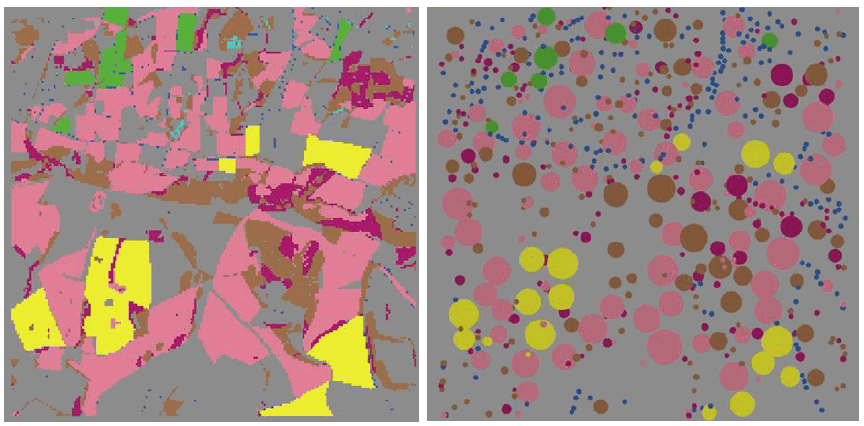
\includegraphics[scale=0.45]{img/new/maps.png}
    \caption{Landšafto žemėlapis (kairėje) ir jo informacijos interpretacija modelyje}
    \label{img:new1}
\end{figure}

Sukurta tikslo funkcija, skaičiuojanti maistingumo reikšmę duotam landšafto žemėlapio pikseliui $x=(x_{x},x_{y})$ \eqref{mapgoal}. Be maistingumo reikšmės matome, jog tikslo funkcijoje naudojamos sinuso ir kosinuso funkcijos. Kadangi landšafto informacija yra vienoda kiekvieno gėlių lauko plote, ši variacija padeda algoritmui išvengti situacijų, kai visi duoti sprendiniai yra vienodi. Papildomai naudojamas labai mažas skaičius $\epsilon$, jog ši variacija nedarytų didelės įtakos galutiniam atsakymui. Duotai landšafto informacijai apskaičiuotos tikslo funkcijos reikšmės vaizdiškai pateiktos 4 priede. 

\begin{equation}\label{mapgoal}
f(x) = \epsilon\sin{(x_{x})}\cos{(x_{y})} - x_{\text{žydėjimo trukmė}}  (x_{\text{žiedadulkės}}x_{\text{žiedadulkių koncentracija}} + x_{\text{nektaras}}x_{\text{nektaro maistinė vertė}}) 
\end{equation}

Kadangi naująjį algoritmą taikome dalykinėje srityje, o ne bendroms optimizavimo užduotims, turime pakeisti algoritmo parametrus ir veikimą, jog šis tiksliau atitiktų tikrų bičių elgesį. 

Iš spietimosi stebėjimų \cite{See10} žinome, jog tik dalis bičių šeimos ieško naujo lizdo spietimosi metu, apie 300-500 bičių dalyvauja procese, todėl taikyme naudosime $CS=500$. Kadangi bitės gali nuskristi tik ribotą atstumą, visuose žingsniuose bitės sprendinių ieškos mažesnėje sprendinių aibėje, sudarytoje iš viso žemėlapio pikselių poaibio, kur pikseliai yra nutolę nuo pradinio lizdo pikselio ne daugiau nei per fiksuotą atstumą $d$.

Panaudoję šią tikslo funkciją su iqsABC algoritmu gauname naują bičių lizdo vietą, į kurią spiesis bitės. Įvykdyti keli bandymai su skirtingais parametrais tikrinant, ar bitės išsirinks palankiausią augalų lauką nektaro ir žiedadulkių atžvilgiu. Rezultatai pateikti~\ref{step1}-ame ir~\ref{step2}-ame paveikslėliuose, čia apskritimu nurodomas paieškos plotas pagal parametrą $d$, o kiekvienas mažesnis raudonas apskritimas yra algoritmo rastas sprendinys kiekvieno bandymo metu. Besispiečiančios šeimos pradinės koordinatės nurodytos su mėlyna žvaigžde.~\ref{step1}-ame paveikslėlyje algoritme naudojamos pradinės šeimos kiekis yra 500, tikslo funkcijų įvertinimų riba 10000. Šiuo atveju šeimos spiečiasi prie geriausiai įvertinto maisto šaltinio.



\begin{figure}
    \centering
    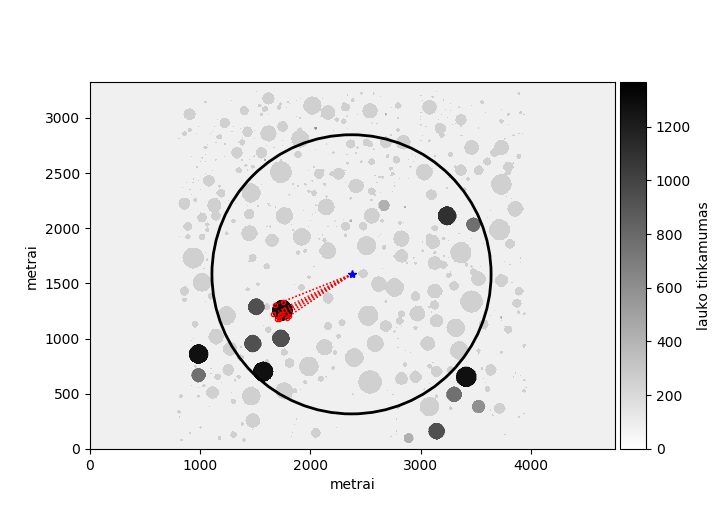
\includegraphics[scale=0.7]{img/new/step1.png}
    \caption{Rezultatai gauti  pritaikius iqsABC su 500 bičių ir 10000 tikslo funkcijos tikrinimų.}
    \label{step1}
\end{figure}

\begin{figure}
    \centering
    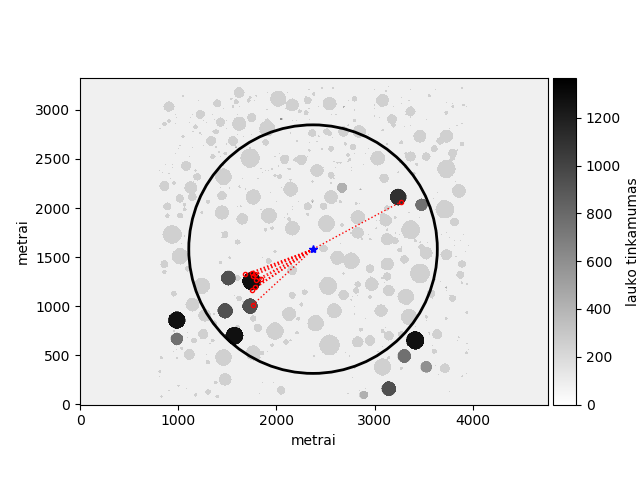
\includegraphics[scale=0.8]{img/new/step2.png}
    \caption{Rezultatai gauti  pritaikius iqsABC su 100 bičių ir 1000 tikslo funkcijos tikrinimų.}
    \label{step2}
\end{figure}


Realybėje spietimosi metu gali pasikeisti oro sąlygos. Jeigu spietimosi metu pradeda lyti, bitės keliaus į lizdą anksčiau, išnagrinėjusios mažiau vietų lizdui. Tokį elgesį galime atkartoti sumažinę tikslo funkcijos įvertinimų kiekį. Algoritmo veikimas su 100 bičių ir tik 1000 tikslo funkcijos įvertinimų pavaizduotas~\ref{step2} paveikslėlyje, matome, jog bitės pasirenka ir kitus maisto šaltinius, įskaitant esančius arčiau lizdo. 




Išbandykime šią tikslo funkciją ir algoritmą kartu su likusiu jungtiniu modeliu. Patenkinus vieną iš spietimosi sąlygų \eqref{ebpss3}, bičių šeima spiečiasi ir ieško naujo lizdo. Iš modelio sABC algoritmas gauna pradines bičių šeimos koordinates ir grąžina naujo lizdo vietą. Pritaikius naująjį algoritmą jungtiniame modelyje matome, jog besispiečiančios bitės iš pasiekiamų laukų pasirenka geriausiai tikslo funkcijos įvertintą augalų lauką (žr.~\ref{img:fin1} pav.). Taip naujasis sABC algoritmas įgyvendina naująjį spietimosi procesą patobulintame modelyje.

\begin{figure}
    \centering
    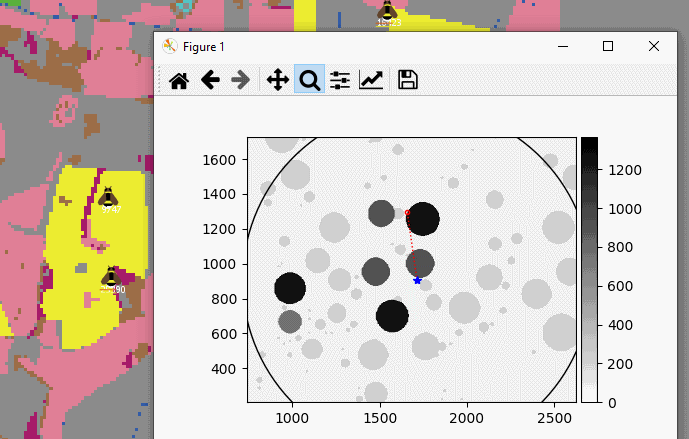
\includegraphics[scale=0.75]{img/new/mags.png}
     \caption{Bičių šeimos spietimasis jungtiniame modelyje}
    \label{img:fin1}
\end{figure}

Bitės spiečiasi sudarydamos naują šeimą rastoje vietoje, palikdamos dalį bičių senojoje šeimoje pagal santykius, naudojamus BEEHAVE modelyje. Kartu spiečius išsineša ir reikalingą maisto atsargų kiekį irgi pagal BEEHAVE modelį, tačiau nauja bičių šeima jau modeliuojama kitoje pozicijoje ir turi prieigą prie kitų maisto šaltinių.

Realybėje bitės atsižvelgtų į papildomus kriterijus, ieškodamos tinkamų medžių drevių arba ieškodamos kitų, anksčiau apleistų, avilių. Gavus išsamesnių landšafto pavyzdžių būtų įmanoma praplėsti tikslo funkciją ir ją pritaikyti išsamesnei informacijai. 

Sukurto modelio išeigos kodas patalpintas GitHub kodo talpykloje \cite{Veg20}. 



\sectionnonum{Rezultatai ir išvados}
% Išvadų ir rekomendacijų dalyje išdėstomi pagrindiniai darbo rezultatai (kažkas
% išanalizuota, kažkas sukurta, kažkas įdiegta), pateikiamos išvados (daromi
% nagrinėtų problemų sprendimo metodų palyginimai, siūlomos rekomendacijos,
% akcentuojamos naujovės).

Darbo metu išanalizavus  esamus bičių populiacijos modelius pastebėta, jog jie neapima visų bitininkystės ir bičių šeimos procesų, tačiau tarp jų yra daug procesų apjungiantis BEEHAVE modelis. Šis modelis gali simuliuoti tik vieną šeimą. Rastas panašus Bumble-BEEHAVE modelis, galintis modeliuoti kelias kamanių šeimas. Jungtinis modelis gautas kelių kamanių šeimų modeliavimą papildžius naminių bičių procesais. Tai buvo atlikta perrašant NetLogo kodą, jog Bumble-Beehave metodai atitiktų naminių bičių, o ne kamanių procesus. Taip buvo sukurtas naujas modelis galintis modeliuoti kelias naminių bičių šeimas vienu metu.

Sukurtas jungtinis modelis toliau buvo tobulinamas procesais, kurie remiasi keliomis arba sukuria naujas bičių šeimas. Įgyvendinti du nauji procesai: bičių migravimas ir bičių spietimasis. Bičių spietimasis jau egzistavo BEEHAVE modelyje, tačiau jis nebuvo susijęs su lizdo pakeitimu ir modeliavo tik vieną šeimą (arba naująją, arba senąją). Pristatytas proceso pakeitimas leidžia modeliuoti spiečiaus naujo lizdo pasirinkimą pagal bičių lizdo ieškojimo ir sprendimo priėmimo procesus.

Kuriant spietimosi procesą sukurti ir išbandyti nauji dirbtinių bičių šeimų algoritmai, paremti natūraliu bičių spietimosi procesu. Vienas iš jų (iqsABC) buvo sukurtas iqABC algoritmo pagrindu, kitas (sABC) ABC pagrindu. Nebuvo statistiškai įrodyta, jog pasiūlyti algoritmai pateiktų geresnius rezultatus nei iqABC algoritmas, tačiau parodyta, jog spietimosi principus pritaikius paprastam ABC algoritmui gauname statistiškai greičiau konverguojantį algoritmą už ABC algoritmą. Jungtinis modelis sėkmingai papildytas sABC algoritmu, sudarius tikslo funkciją iš aplinkos modelio informacijos ir pakeitus sprendinių aibę.

Iš gautų rezultatų daromos šios išvados:
\begin{enumerate}
    \item Iš dabartinių BEEHAVE ir Bumble-BEEHAVE bitininkystės procesų modelių įmanoma sudaryti kelias naminių bičių šeimas simuliuojantį modelį.
    \item Kelias bičių šeimas apimantis modelis suteikia galimybę jį toliau tobulinti pridedant tarpšeimyninius bičių procesus, tačiau šie procesai tarpusavyje gali būti reikšmingai susiję. Pagal empirines žinias ir tyrimus bičių migracija keičiasi pagal varozės procesus.
    \item Dirbtinių bičių šeimų algoritmai gali būti sėkmingai tobulinami bičių spietimosi principu, o ne vien maisto paieškos principu.
    \item Dirbtinių bičių šeimų algoritmai sėkmingai pritaikomi bitininkystės modeliavimo srityje.
\end{enumerate}


Darbo metu sukurtą modelį galima būtų tobulinti literatūros analizės metu išskirtu varozės plitimo tarp šeimų procesu ir išsamesniu klimato įtakos bitėms modeliu. Pritaikius varozės plitimo procesus būtų galima patobulinti pristatyto modelio bičių migracijos procesą.

% Iš šių procesų bičių migracijos procesas, nors ir įgyvendintas, gali remtis tik šaltinyje pateikta statistine informacija ir nesiremia ilgalaikių stebėjimų empiriniais duomenimis.

% Nors dėl tyrinėjamos dalykinės srities didžioji dalis žinių susijusi tik su apiologijos sritimi, kompiuterinio modelio kūrimas ir procesų įgyvendinimas leido sukurti naujų žinių metaeuristinių algoritmų srityje.


Sukurtą naują iqsABC algoritmą būtų galima išbandyti su kitais skirtingais parametrais ir nustatyti kitokius sprendinio tikrinimo kriterijus. Taip pat būtų galima palyginti naujus iqsABC ir sABC algoritmus su kitais dirbtinių bičių šeimos algoritmais. Pavyzdžiui, iš konvergavimo diagramų matome įdomų qABC ir sABC konvergavimo santykį, kuris nebuvo tirtas šiame darbe. Pristatytus algoritmus galima ištirti ir naudojant daugiau skirtingų tikslo funkcijų.

% Literatūros analizės metu išskirti papildomi procesai, kuriais galima toliau tobulinti pateiktą jungtinį modelį. Šie procesai yra:
% \begin{enumerate}
%     \item Varozės plitimas tarp kelių bičių šeimų
%     \item Išsamesnis klimato poveikio modelis bičių šeimoms
% \end{enumerate}

% Iš šių procesų bičių migracijos procesas, nors ir įgyvendintas, gali remtis tik šaltinyje pateikta statistine informacija ir nesiremia ilgalaikių stebėjimų empiriniais duomenimis.

% Nors dėl tyrinėjamos dalykinės srities didžioji dalis žinių susijusi tik su apiologijos sritimi, kompiuterinio modelio kūrimas ir procesų įgyvendinimas leido sukurti naujų žinių metaeuristinių algoritmų srityje.

























% Plačiau apie šaltinių tipus ir jų atributus:
% http://mirror.datacenter.by/pub/mirrors/CTAN/macros/latex/contrib/biblatex/doc/biblatex.pdf#subsection.2.1

\printbibliography[heading=bibintoc]  

% Šaltinių sąraše abėcėlės tvarka
% išdėstomi darbe panaudotų (cituotų, perfrazuotų ar bent paminėtų) mokslo
% leidinių, kitokių publikacijų bibliografiniai aprašai. Aprašai pateikiami
% netransliteruoti.

\renewcommand{\appendixname}{}

\appendix  % Priedai
% Prieduose pateikiami programų tekstai, lentelės, schemos, paveiksliukai ir
% kita papildoma medžiaga, kuri yra papildanti darbo turinį. Jeigu lentelės,
% paveiksliukai yra nedideli ir jų nedaug, jie turi būti pateikti pagrindinėje
% dalyje.





\begin{landscape}

\section{Konvergavimo grafikai su iqABC ir iqsABC}\label{PR1}

\begin{multicols}{2}

\begin{figure}[H]
    \centering
    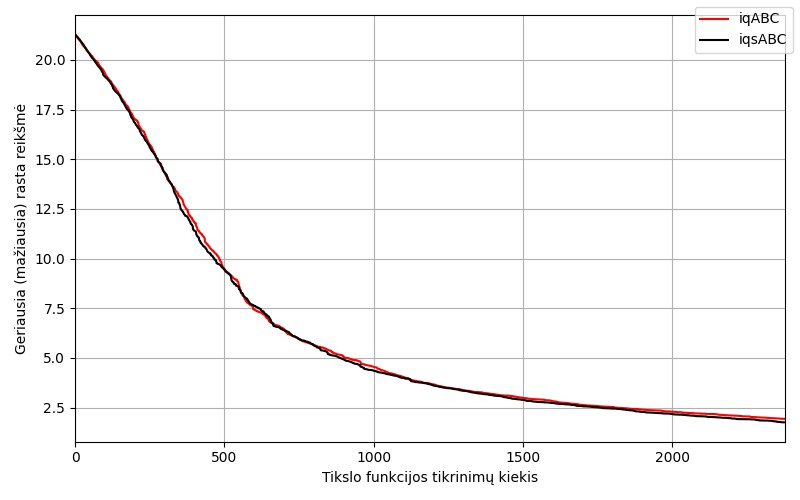
\includegraphics[scale=0.5]{img/2kg/ackley.jpg}
    \caption{Algoritmų konvergavimas su Ackley tikslo funkcija}
    \label{img:vkon1}
\end{figure}

\begin{figure}[H]
    \centering
    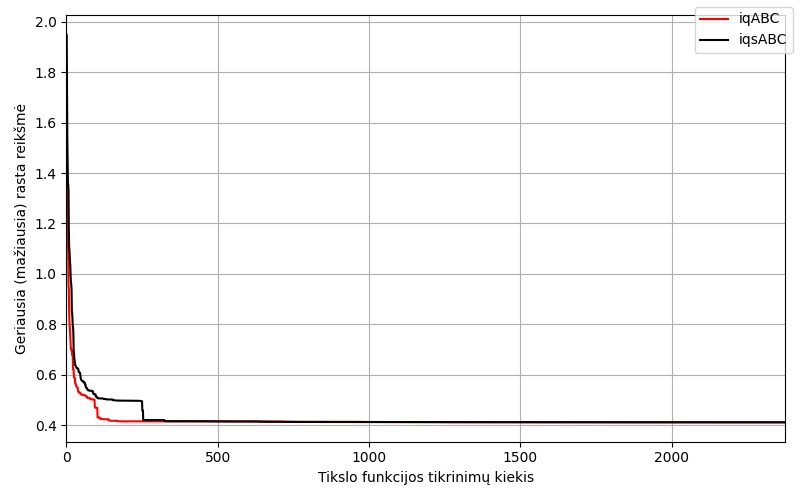
\includegraphics[scale=0.5]{img/2kg/branin.jpg}
     \caption{Algoritmų konvergavimas su Branin tikslo funkcija}
    \label{img:vkon2}
\end{figure}

\end{multicols}
\begin{multicols}{2}

\begin{figure}[H]
    \centering
    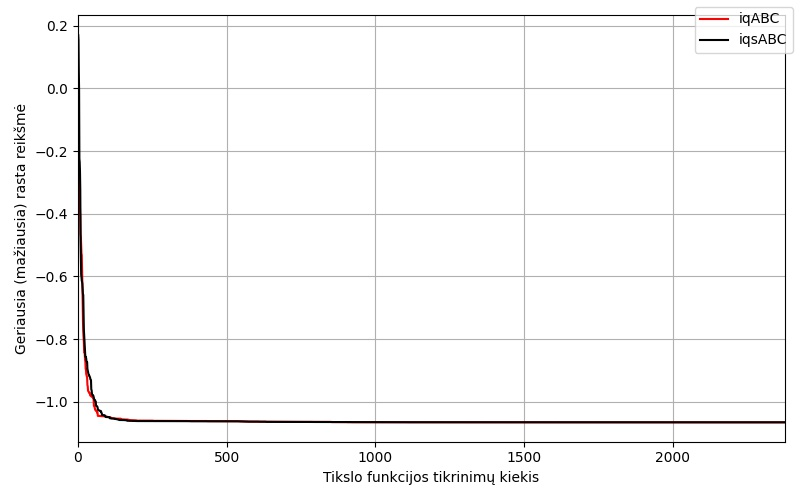
\includegraphics[scale=0.45]{img/2kg/camel.jpg}
     \caption{Algoritmų konvergavimas su kupranugario tikslo funkcija}
    \label{img:vkon3}
\end{figure}

\begin{figure}[H]
    \centering
    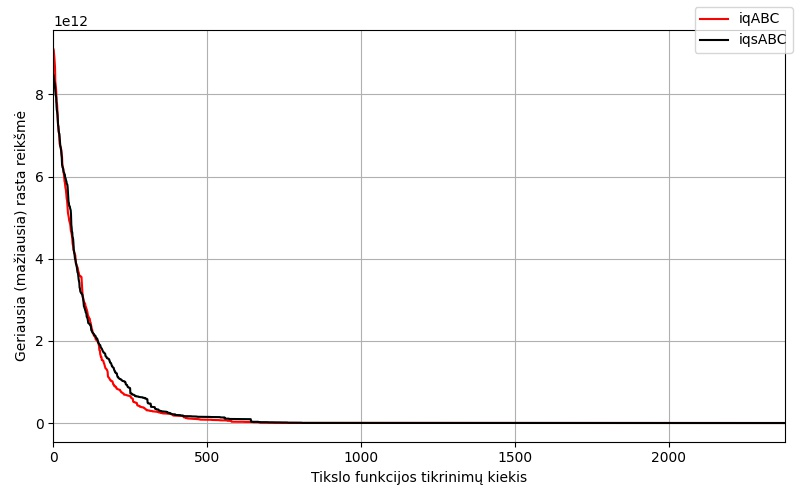
\includegraphics[scale=0.45]{img/2kg/dixon.jpg}
     \caption{Algoritmų konvergavimas su Dixon tikslo funkcija}
    \label{img:vkon4}
\end{figure}

\end{multicols}\newpage
\begin{multicols}{2}

\begin{figure}[H]
    \centering
    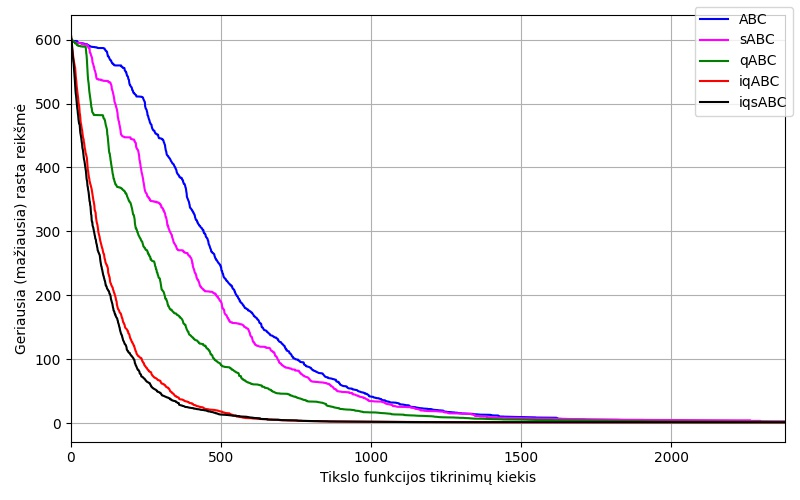
\includegraphics[scale=0.45]{img/2kv/all_griewank.jpg}
     \caption{Algoritmų konvergavimas su Griewank tikslo funkcija}
    \label{img:vkon5a}
\end{figure}

\begin{figure}[H]
    \centering
    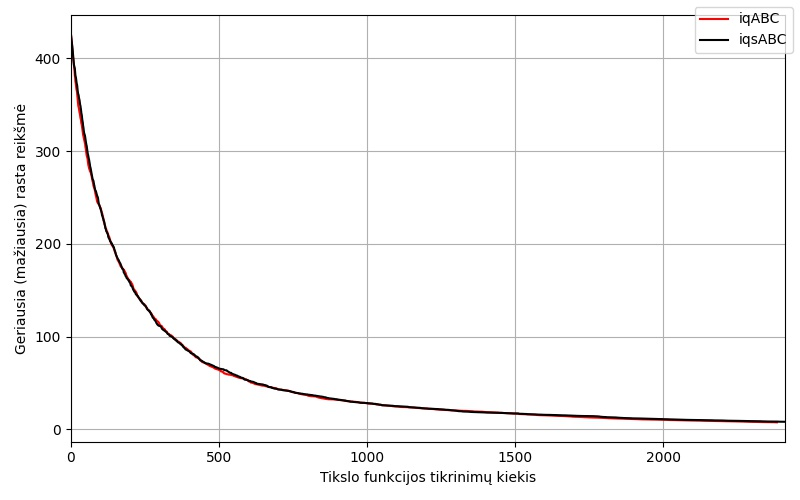
\includegraphics[scale=0.5]{img/2kg/rastrigin.jpg}
     \caption{Algoritmų konvergavimas su Rastrigin tikslo funkcija}
    \label{img:vkon5}
\end{figure}



\end{multicols}
\begin{multicols}{2}

\begin{figure}[H]
    \centering
    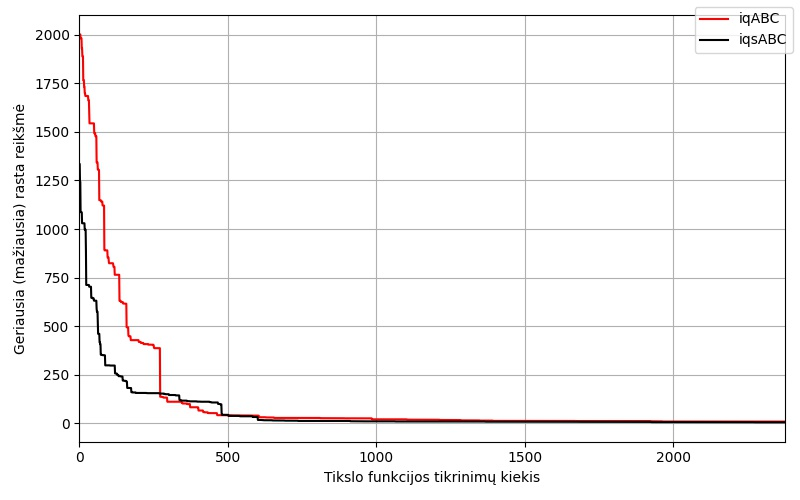
\includegraphics[scale=0.5]{img/2kg/rosenbrock.jpg}
     \caption{Algoritmų konvergavimas su Rosenbrock tikslo funkcija}
    \label{img:vkon6}
\end{figure}

\begin{figure}[H]
    \centering
    \includegraphics[scale=0.5]{img/2kg/Schaffer.jpg}
     \caption{Algoritmų konvergavimas su Schaffer tikslo funkcija}
    \label{img:vkon7}
\end{figure}


\end{multicols}\newpage
\begin{multicols}{2}


\begin{figure}[H]
    \centering
    \includegraphics[scale=0.5]{img/2kg/Schwefel.jpg}
     \caption{Algoritmų konvergavimas su Schwefel tikslo funkcija}
    \label{img:vkon8a}
\end{figure}



\begin{figure}[H]
    \centering
    \includegraphics[scale=0.5]{img/2kg/Sphere.jpg}
     \caption{Algoritmų konvergavimas su sferos tikslo funkcija}
    \label{img:vkon8}
\end{figure}




\end{multicols}
\begin{multicols}{2}


\begin{figure}[H]
    \centering
    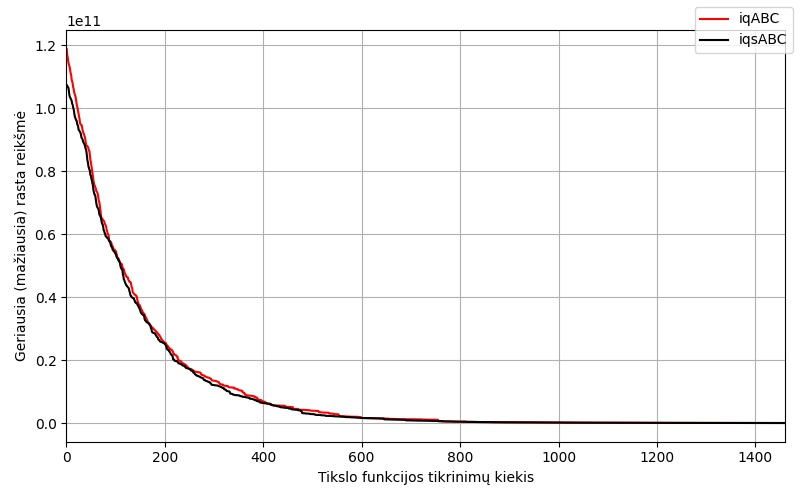
\includegraphics[scale=0.5]{img/2kg/f1.jpg}
    \caption{Algoritmų konvergavimas su $f_{1}$ tikslo funkcija}
    \label{img:vkonf1}
\end{figure}

\begin{figure}[H]
    \centering
    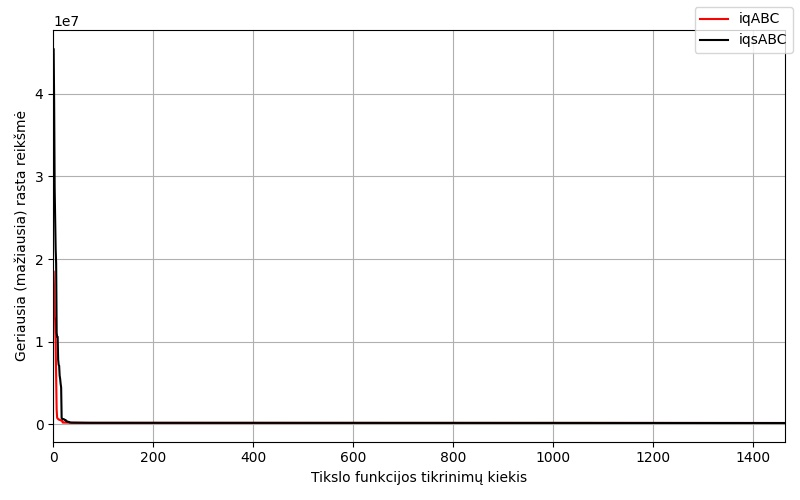
\includegraphics[scale=0.5]{img/2kg/f2.jpg}
    \caption{Algoritmų konvergavimas su $f_{2}$ tikslo funkcija}
    \label{img:vkonf2}
\end{figure}




\end{multicols}\newpage
\begin{multicols}{2}


\begin{figure}[H]
    \centering
    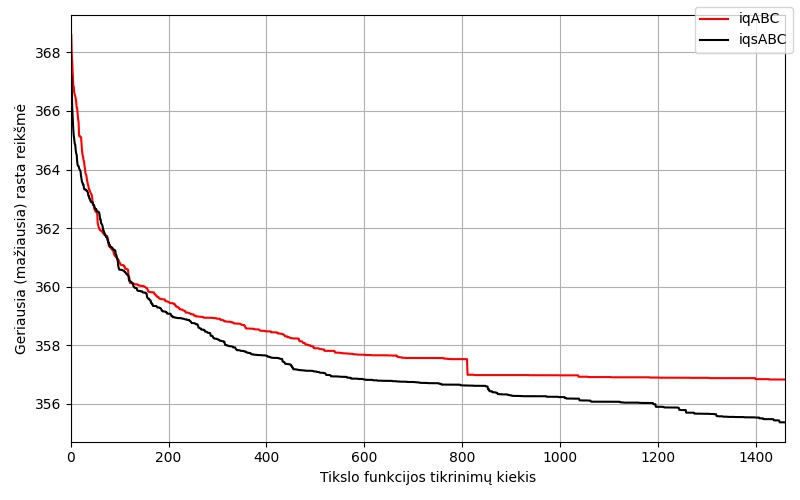
\includegraphics[scale=0.5]{img/2kg/f3.jpg}
    \caption{Algoritmų konvergavimas su $f_{3}$ tikslo funkcija}
    \label{img:vkonf3}
\end{figure}

\begin{figure}[H]
    \centering
    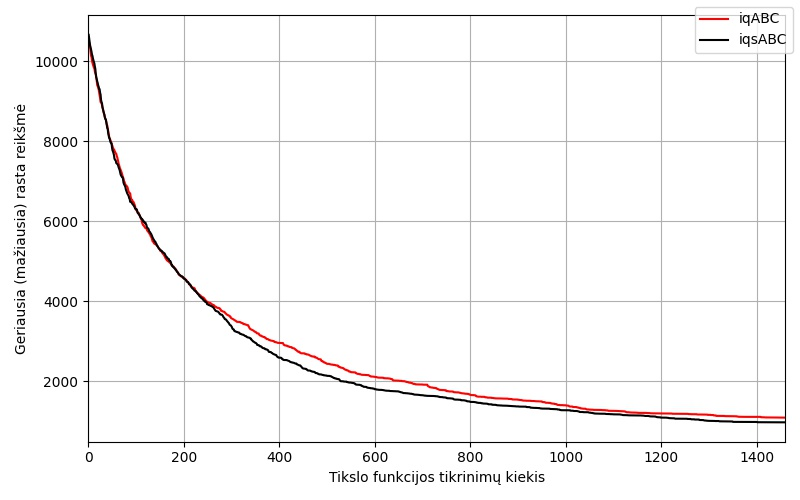
\includegraphics[scale=0.5]{img/2kg/f4.jpg}
    \caption{Algoritmų konvergavimas su $f_{4}$ tikslo funkcija}
    \label{img:vkonf4}
\end{figure}





\end{multicols}
\begin{multicols}{2}


\begin{figure}[H]
    \centering
    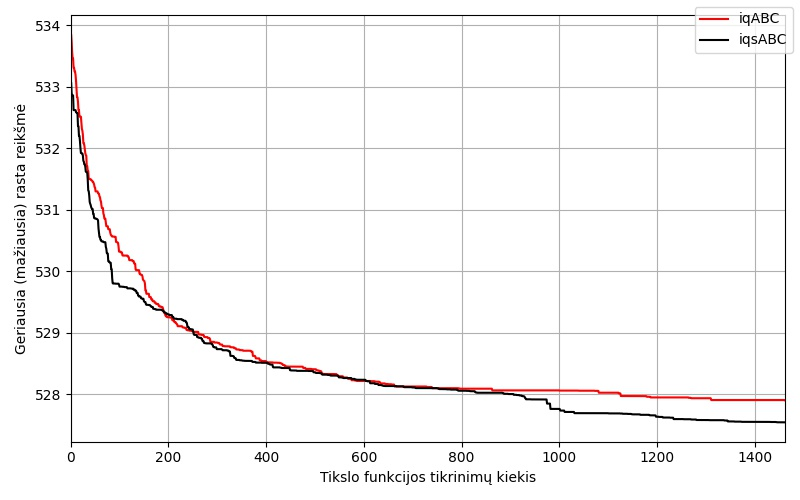
\includegraphics[scale=0.5]{img/2kg/f5.jpg}
    \caption{Algoritmų konvergavimas su $f_{5}$ tikslo funkcija}
    \label{img:vkonf5}
\end{figure}

\begin{figure}[H]
    \centering
    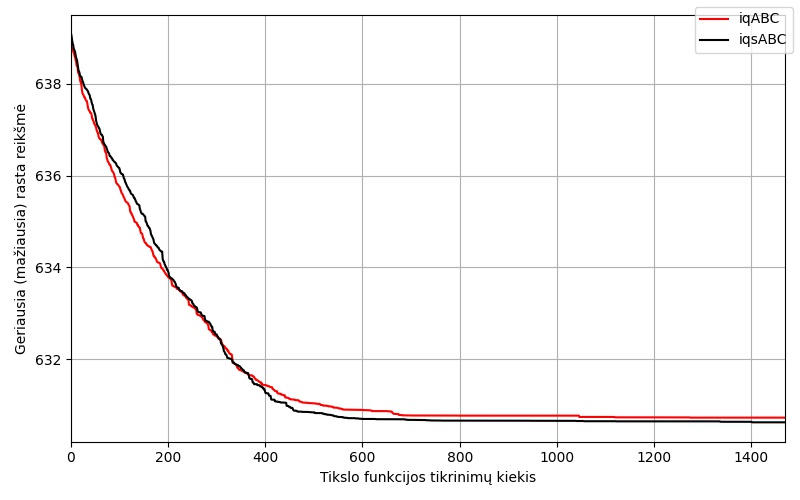
\includegraphics[scale=0.5]{img/2kg/f6.jpg}
    \caption{Algoritmų konvergavimas su $f_{6}$ tikslo funkcija}
    \label{img:vkonf6}
\end{figure}





\end{multicols}\newpage
\begin{multicols}{2}


\begin{figure}[H]
    \centering
    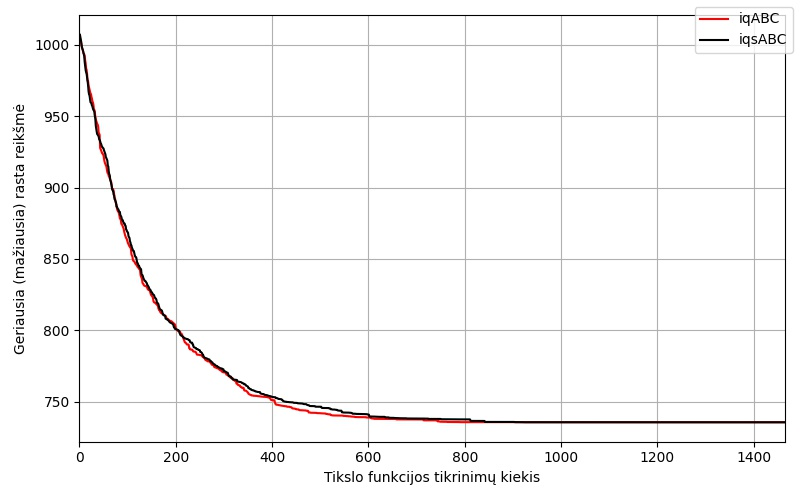
\includegraphics[scale=0.5]{img/2kg/f7.jpg}
    \caption{Algoritmų konvergavimas su $f_{7}$ tikslo funkcija}
    \label{img:vkonf7}
\end{figure}


\begin{figure}[H]
    \centering
    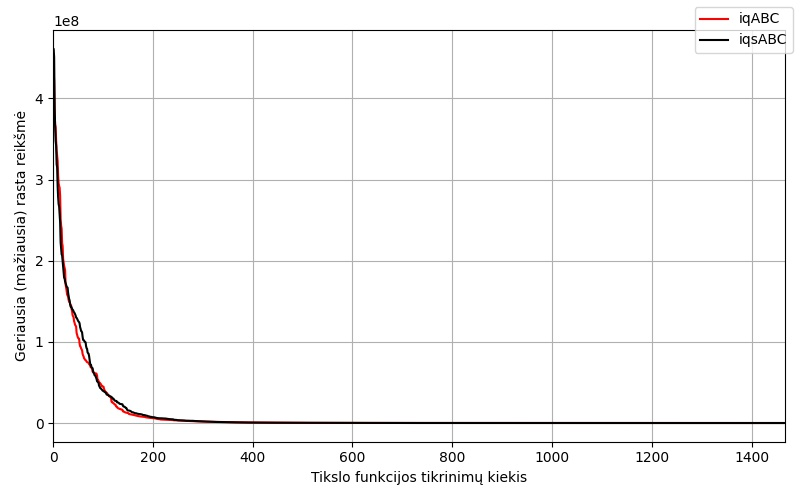
\includegraphics[scale=0.5]{img/2kg/f8.jpg}
    \caption{Algoritmų konvergavimas su $f_{8}$ tikslo funkcija}
    \label{img:vkonf8}
\end{figure}



\end{multicols}
\begin{multicols}{2}


\begin{figure}[H]
    \centering
    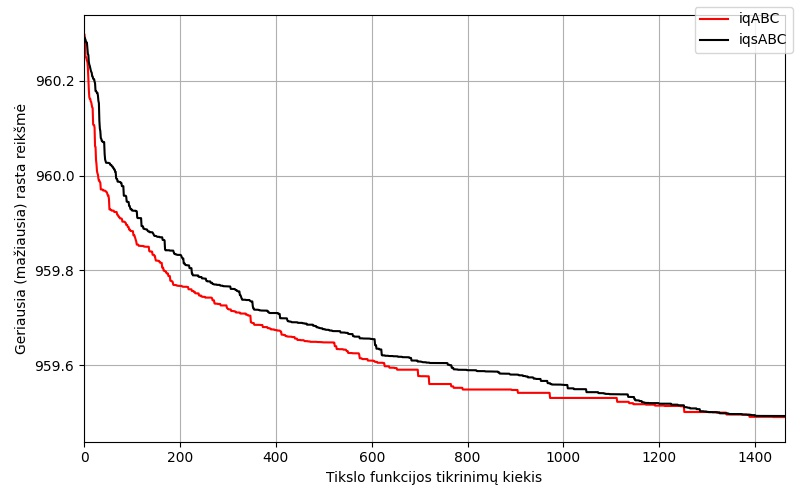
\includegraphics[scale=0.5]{img/2kg/f9.jpg}
    \caption{Algoritmų konvergavimas su $f_{9}$ tikslo funkcija}
    \label{img:vkonf9}
\end{figure}


\begin{figure}[H]
    \centering
    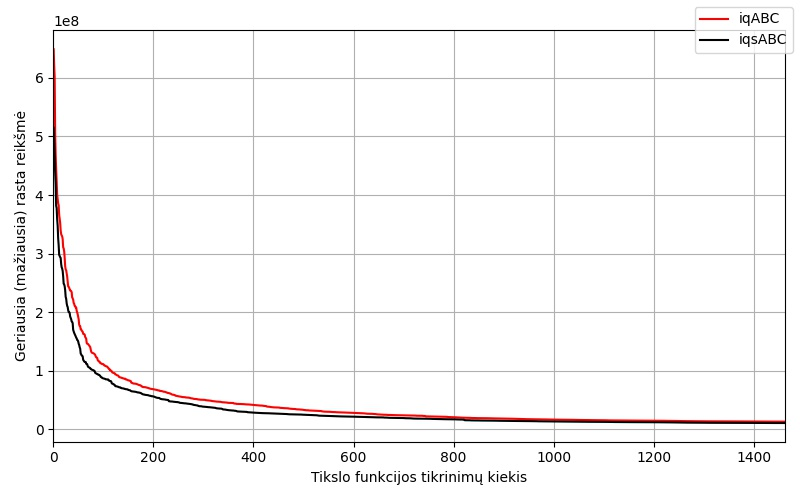
\includegraphics[scale=0.5]{img/2kg/f10.jpg}
    \caption{Algoritmų konvergavimas su $f_{10}$ tikslo funkcija}
    \label{img:vkonf10}
\end{figure}




\end{multicols}\newpage
\begin{multicols}{2}


\begin{figure}[H]
    \centering
    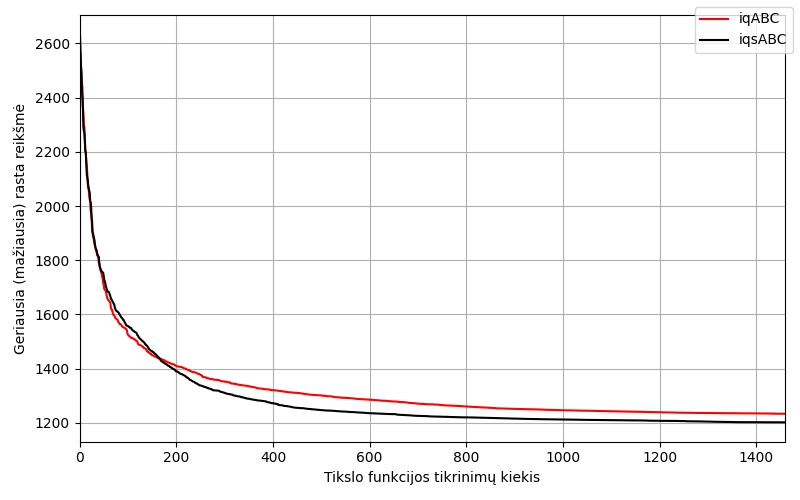
\includegraphics[scale=0.5]{img/2kg/f11.jpg}
    \caption{Algoritmų konvergavimas su $f_{11}$ tikslo funkcija}
    \label{img:vkonf11}
\end{figure}

\begin{figure}[H]
    \centering
    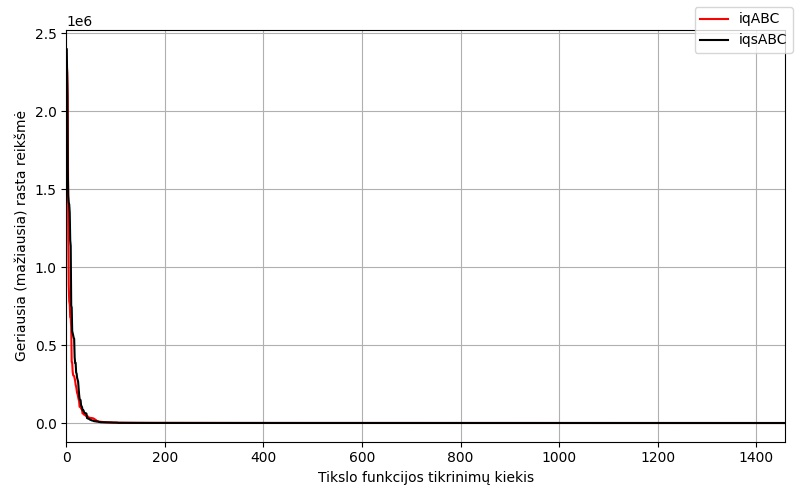
\includegraphics[scale=0.5]{img/2kg/f12.jpg}
    \caption{Algoritmų konvergavimas su $f_{12}$ tikslo funkcija}
    \label{img:vkonf12}
\end{figure}






\end{multicols}
\begin{multicols}{2}

\begin{figure}[H]
    \centering
    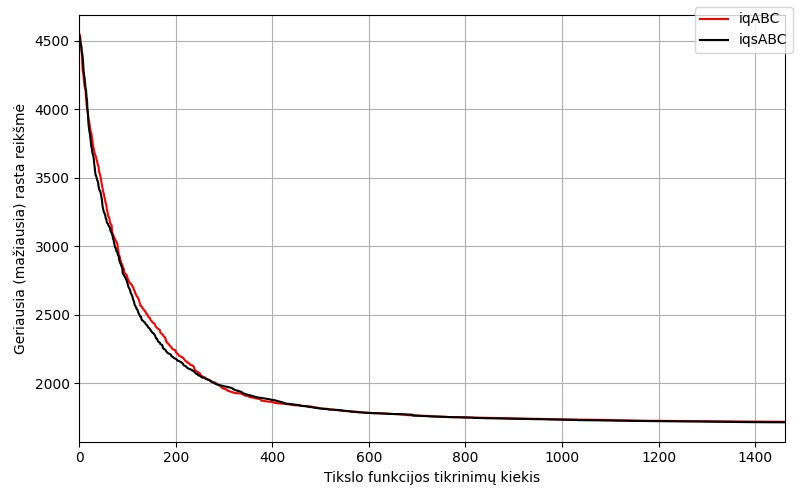
\includegraphics[scale=0.5]{img/2kg/f13.jpg}
    \caption{Algoritmų konvergavimas su $f_{13}$ tikslo funkcija}
    \label{img:vkonf13}
\end{figure}

\begin{figure}[H]
    \centering
    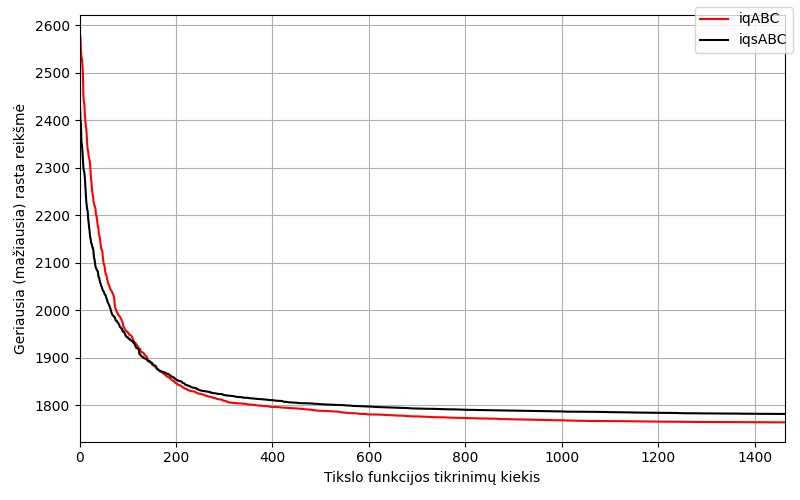
\includegraphics[scale=0.5]{img/2kg/f14.jpg}
    \caption{Algoritmų konvergavimas su $f_{14}$ tikslo funkcija}
    \label{img:vkonf14}
\end{figure}


\end{multicols}


\begin{figure}[H]
    \centering
    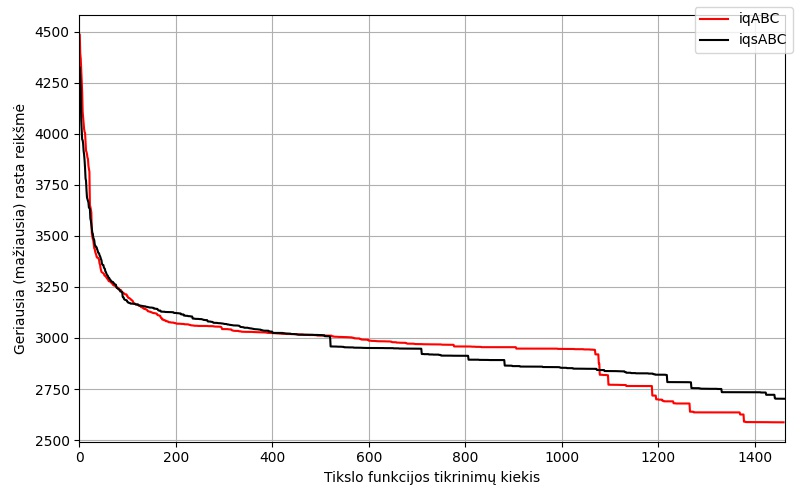
\includegraphics[scale=0.5]{img/2kg/f15.jpg}
    \caption{Algoritmų konvergavimas su $f_{15}$ tikslo funkcija}
    \label{img:vkonf15}
\end{figure}

\end{landscape}








\section{Kiti iqsABC ir sABC algoritmų tyrimo rezultatai}\label{PR2eff}




Paskutiniai rezultatai
\begin{table}[H]
\centering
\small
\caption{iqsABC algoritmo efektyvumas kai $D=30$ (2500 tikslo funkcijos skaičiavimų)}
\npdecimalsign{,}
\nprounddigits{3} 
\begin{tabular}{p{0.1\linewidth} r n{8}{3} n{8}{3} n{8}{3} X}
Tikslo funkcija & Algoritmas & Min & Max & Vidurkis & Standartinis nuokrypis \\
\hline
Ackley& iqABC & 1.08182574826888 & 2.4961238639921355 & 1.8268667740842852 & 0.38362196915311414\\
Ackley& iqsABC & 0.7840931032980585 & 2.7335880698501036 & 1.7875261496002883 & 0.45872040194711566\\
Branin & iqABC & 0.397887463531184 & 0.3984217863892425 & 0.41121611432821525 & 0.00010679594941363753\\
Branin & iqsABC & 0.39788743446703023 & 0.39855002761877145 & 0.41121184778870107 & 0.00013236324718124109\\
Camel & iqABC & -1.0316284403544957 & 0 & -1.0316284403544957 & 1.217751357145945e-05\\
Camel & iqsABC & -1.0316284403544957 & -1.0316284403544957 & -1.0316284403544957 & 1.2508837439010842e-05\\
Dixon & iqABC & 14205.8602351473 & 7904341.353030231 & 1090818.5293888415 & 1517509.3522839383\\
Dixon & iqsABC & 43717.7516385791 & 1400632.9517081555 & 696546.6849277939 & 379541.6632869636\\
Griewank & iqABC & 1.023769492027791 & 1.1855620636877648 & 1.1049192733816269 & 0.034840663639525045\\
Griewank & iqsABC & 1.026601549273476 & 1.1528674009010595 & 1.1076003452745797 & 0.02850600600595648\\
Rastrigin & iqABC & 3.85659093149874 & 10.848533052698983 & 7.823900860225207 & 2.0890934684970603\\
Rastrigin & iqsABC & 2.902090263244844 & 11.344688204381832 & 8.238307342429794 & 2.050308645850677\\
Rosenbrock & iqABC & 0.03127157275145096 & 30.9620465567142 & 7.567063379586808 & 7.734127397482404\\
Rosenbrock & iqsABC & 0.18681998576425166 & 38.05751919668468 & 8.530676842579417 & 9.68115155214303\\
Schaffer & iqABC & 0.0016341389191246725 & 0.028786436618562283 & 0.01126470869578542 & 0.004294835970215177\\
Schaffer & iqsABC & 0.00017491384775081276 & 0.037227506158084234 & 0.010938221319810636 & 0.005280109235753065\\
Schwefel & iqABC & -11405.911979417826 & -9331.274596354578 & -11330.278596354578 & 254.94504588513496\\
Schwefel & iqsABC & -11390.170084514542 & -9127.374791354578 & -10241.600634619212 & 603.483720206225\\
Sphere & iqABC & 2.204296277254379 & 16.943114814667247 & 7.97155932665491 & 3.581994483218065\\
Sphere & iqsABC & 2.5136866104806703 & 55.343040313333006 & 9.21078645243229 & 9.189298843854923
\end{tabular}
\end{table}



%Paskutiniai rezultatai
\begin{table}[H]
\centering
\small
\caption{iqsABC algoritmo efektyvumas kai $D=30$ (1500 tikslo funkcijos skaičiavimų)}
\npdecimalsign{,}
\nprounddigits{3} 
\begin{tabular}{p{0.1\linewidth} r n{8}{3} n{8}{3} n{8}{3} X}
Tikslo funkcija & Algoritmas & Min & Max & \text{Vidurkis} & Standartinis nuokrypis \\
\hline
f1 & iqABC & 29404854.726960767 & 1513001999.886286 & 211996760.47225928 & 367385927.9928144 \\
f1 & iqsABC & 16585381.394055143 & 952639554.9634097 & 106582996.94978577 & 197457483.15937597 \\
f2 & iqABC & 92986.67473081044 & 202215.86839061824 & 154055.69086129236 & 29592.24019889139 \\
f2 & iqsABC & 93251.4613983864 & 197176.82602256298 & 146680.15441418826 & 23765.39978340099 \\
f3 & iqABC & 334.1122038554841 & 345.5463389266071 & 357.6258289765807 & 3.2370272560307463 \\
f3 & iqsABC & 330.8452452438729 & 343.2594705085195 & 354.9510817979323 & 3.011282435138136 \\
f4 & iqABC & 618.0396365662382 & 2218.136376938779 & 1163.5047425435532 & 401.3850845407521 \\
f4 & iqsABC & 633.431863738826 & 2253.3148008153366 & 1181.0212215056947 & 359.5100372626863 \\
f5 & iqABC & 501.3777122156415 & 503.5341035752996 & 527.5961072305644 & 0.6867746301692887 \\
f5 & iqsABC & 501.1425892389035 & 503.6701749270449 & 527.4070584007048 & 0.7062487775261981 \\
f6 & iqABC & 600.4613714583053 & 600.9254752452833 & 630.6841091540225 & 0.12880311668089878 \\
f6 & iqsABC & 600.2617014925529 & 600.8874832851961 & 630.5968348926017 & 0.14594645755873195 \\
f7 & iqABC & 700.2935881782455 & 702.9105032410323 & 735.7710239123319 & 0.5686080540617086 \\
f7 & iqsABC & 700.2496144974169 & 701.2142262526827 & 735.5927043987056 & 0.2566173083049533 \\
f8 & iqABC & 843.1784834570765 & 1827.0233029594904 & 1173.7495746166999 & 290.0125686016902 \\
f8 & iqsABC & 842.5775357644591 & 3402.837623678488 & 1401.0853996109308 & 663.7472874595333 \\
f9 & iqABC & 912.6280502300087 & 914.0212301992864 & 959.3270470455485 & 0.3661020152917745 \\
f9 & iqsABC & 913.010993236272 & 914.4224842170296 & 959.5070753247976 & 0.30168122870072434 \\
f10 & iqABC & 3270279.4219501903 & 36192496.93182283 & 11595189.82185725 & 8010253.044419424 \\
f10 & iqsABC & 1671791.6102617802 & 33707495.648108125 & 11968755.123495964 & 8337741.365283647 \\
f11 & iqABC & 1124.373746502472 & 1308.2111450859818 & 1222.0971523920964 & 51.23154922172501 \\
f11 & iqsABC & 1121.9047356663907 & 1296.6252472928743 & 1230.647685217731 & 50.19670984985638 \\
f12 & iqABC & 1478.8520410665062 & 2895.249367905626 & 2187.4810275661657 & 314.37859723277785 \\
f12 & iqsABC & 1659.333973482483 & 2834.963471984872 & 2293.5903440537795 & 252.4708799028634 \\
f13 & iqABC & 1640.4350460158637 & 1768.301555306535 & 1788.3140257647524 & 33.026630799778786 \\
f13 & iqsABC & 1643.3042921203173 & 1780.4281696678727 & 1760.5447131879544 & 29.570876099420108 \\
f14 & iqABC & 1641.5636251206383 & 1772.548636567436 & 1775.5041274705043 & 33.93432674160527 \\
f14 & iqsABC & 1635.8045907691328 & 1866.6420178921237 & 1784.846913926081 & 56.140731724486685 \\
f15 & iqABC & 1909.8020771425977 & 2980.9304546646517 & 2407.680832411329 & 376.05547505349205 \\
f15 & iqsABC & 1903.3862719494991 & 2980.1554391738355 & 2383.430157392349 & 398.9058452158306
\end{tabular}
\end{table}







%Paskutiniai rezultatai
\begin{table}[H]
\centering
\small
\caption{iqsABC algoritmo efektyvumas kai $D=30$ (500000 tikslo funkcijos skaičiavimų)}
\npdecimalsign{,}
\nprounddigits{3}
\begin{tabular}{p{0.1\linewidth} r n{8}{3} n{8}{3} n{8}{3} X}
Tikslo funkcija & Algoritmas & Min & Max & \text{Vidurkis} & Standartinis nuokrypis \\
\hline
Ackley& iqABC & 2.842170943040401e-14 & 3.907985046680551e-14 & 3.327708479143136e-14 & 3.1688046344554865e-15\\
Ackley& iqsABC & 2.1316282072803006e-14 & 3.907985046680551e-14 & 3.529028920941831e-14 & 4.648793688107493e-15\\
Branin & iqABC & 0.39788735772973816 & 0.39788735772973816 & 0.39788735772973816 & 0.0\\
Branin & iqsABC & 0.39788735772973816 & 0.39788735772973816 & 0.39788735772973816 & 0.0\\
Camel & iqABC & -1.0316284534898779 & -1.0316284534898779 & -1.0316284534898779 & 4.094300213216723e-16\\
Camel & iqsABC & -1.0316284534898779 & -1.0316284534898779 & -1.0316284534898779 & 4.213000162292041e-16\\
Dixon & iqABC & 0.004502895408584585 & 14.299125057996392 & 1.6642395528043867 & 2.8929905928488\\
Dixon & iqsABC & 0.0024548914574172337 & 7.8460444817694945 & 0.9750927555852758 & 1.6023926149440022\\
Griewank & iqABC & 0.0 & 1.1102230246251565e-16 & 1.850371707708594e-17 & 3.774032578002451e-17\\
Griewank & iqsABC & 0.0 & 1.1102230246251565e-16 & 4.070817756958907e-17 & 5.3501026922775204e-17\\
Rastrigin & iqABC & 0.0 & 0 & 0.0 & 0.0\\
Rastrigin & iqsABC & 0.0 & 0 & 0.0 & 0.0\\
Rosenbrock & iqABC & 0.0001908333808193178 & 0.0364928834891299 & 0.008933115696698092 & 0.008399979945706617\\
Rosenbrock & iqsABC & 1.2472342327067042e-05 & 0.034179299555925476 & 0.007737530806525839 & 0.00888316373963952\\
Schaffer & iqABC & 0.0 & 6.206490377191898e-08 & 9.214494419336934e-09 & 1.651688597992383e-08\\
Schaffer & iqsABC & 0.0 & 8.629492809220096e-08 & 1.0516989338663999e-08 & 2.2166196258462983e-08\\
Schwefel & iqABC & -12569.486618173014 & -12569.486618173014 & -12569.486618173014 & 5.752149554916067e-13\\
Schwefel & iqsABC & -12569.486618173014 & -12569.486618173014 & -12569.486618173014 & 5.752149554916067e-13\\
Sphere & iqABC & 2.722231101572975e-16 & 4.962653651272573e-16 & 3.908564165510869e-16 & 7.6234570887757e-17\\
Sphere & iqsABC & 2.7146871704022266e-16 & 4.956170267095344e-16 & 3.723584239937519e-16 & 6.71133723676196e-17
\end{tabular}
\end{table}





%Paskutiniai rezultatai
\begin{table}[H]
\centering
\small
\caption{iqsABC algoritmo efektyvumas kai $D=30$ (500000 tikslo funkcijos skaičiavimų)}
\begin{tabular}{p{0.1\linewidth} r S S S X}
Tikslo funkcija & Algoritmas & Min & Max & \text{Vidurkis} & Standartinis nuokrypis \\
\hline
%f1 ir f5 ir f11 ir f15 senesni
f1 & iqABC & 132.1803656 & 2491.631441 & 684.3384766 & 541.3079583402091 \\
f1 & iqsABC & 145.4542366 & 2030.198565 & 681.7975297 & 438.4267458473861 \\
f2 & iqABC & 63437.44660846651 & 111112.04833061455 & 85671.3352655965 & 9661.381481175054\\
f2 & iqsABC & 59309.2891533273 & 105971.35189104071 & 91350.48818142178 & 10814.509024055798\\
f3 & iqABC & 310.4773185404185 & 332.27170369901677 & 338.7920980558421 & 3.890190739119788\\
f3 & iqsABC & 302.51811591901617 & 333.449190674848 & 338.9914097976573 & 6.458018663544821\\
f4 & iqABC & 279.7012289297454 & 400.2706538884595 & 409.4790942301688 & 21.622472040815033\\
f4 & iqsABC & 400.06247258207077 & 400.2498325043507 & 413.48256387660246 & 0.04998290302224157\\
f5 & iqABC & 500.388117 & 500.8814412 & 500.5513874 & 0.10556727978483932 \\
f5 & iqsABC & 500.1786207 & 500.7328268 & 500.589256 & 0.12972795187766062 \\
f6 & iqABC & 600.0894178408205 & 600.2149548992851 & 620.181841397527 & 0.02628630745833276\\
f6 & iqsABC & 600.1223070638856 & 600.2282489012099 & 620.1815458074178 & 0.022725496582467926\\
f7 & iqABC & 700.1478227222589 & 700.2334793119386 & 723.5319308979832 & 0.02301732698108637\\
f7 & iqsABC & 700.1407691001829 & 700.2481117728486 & 723.5400729664964 & 0.02917483500121372\\
f8 & iqABC & 804.4190474347889 & 820.8463344509452 & 842.9471283864699 & 3.8158613984573666\\
f8 & iqsABC & 806.147350081779 & 822.1961585926822 & 843.6636416382669 & 4.325286911243914\\
f9 & iqABC & 911.7378153505035 & 913.0025858561771 & 942.9913514177048 & 0.2927941683099912\\
f9 & iqsABC & 912.1972235453657 & 912.9107059549522 & 943.0146134526044 & 0.20398919705843332\\
f10 & iqABC & 122092.67634805532 & 809639.2767113815 & 410473.7762125953 & 166929.95512085748\\
f10 & iqsABC & 78003.00591232692 & 835041.7020980772 & 447850.3781497507 & 170472.31764255735\\
f11 & iqABC & 1114.887631 & 1119.522142 & 1118.153814 & 1.0873610226907342 \\
f11 & iqsABC & 1113.89049 & 1119.260414 & 1117.298634 & 1.3495040974264993 \\
f12 & iqABC & 1284.1455695841935 & 1651.6250107808164 & 1487.9771680451433 & 84.22930339457994\\
f12 & iqsABC & 1287.3009188236163 & 1666.8170590169964 & 1494.6137735827012 & 95.62946560208009\\
f13 & iqABC & 1574.6144354134647 & 1627.6444671447998 & 1663.5083347680206 & 15.373957910387482\\
f13 & iqsABC & 1572.8178540044228 & 1627.6440056817205 & 1657.4918839474715 & 17.482831624195917\\
f14 & iqABC & 1609.1849203663783 & 1623.9450304827774 & 1670.4659427166052 & 4.240557842345996\\
f14 & iqsABC & 1611.4127924700736 & 1629.678536367082 & 1672.757429586367 & 4.148163861355185\\
f15 & iqABC & -39791.001923071046 & 1912.2344929632 & 554.6451673200206 & 7481.186148480018\\
f15 & iqsABC & 1900.0899565985787 & 1906.171489001923 & 1964.7868630318378 & 1.706260136797319
\end{tabular}
\end{table}


%Paskutiniai rezultatai

\begin{table}[H]
\centering
\small
\caption{sABC algoritmo efektyvumas kai $D=30$ (1500 tikslo funkcijos skaičiavimų)}
\label{tab:nsmall}
\npdecimalsign{,}
\nprounddigits{3}
\begin{tabular}{l|l| n{13}{3}| n{4}{3}}
% Tikslo funkcija & \makecell{Statistiškai geresnis \\ algoritmas} & \makecell{Atsakymo vidurkio \\ skirtumas ABC-sABC} & p reikšmė \\
 Tikslo funkcija & Statistiškai geresnis & \text{Atsakymo vidurkio} & \text{p reikšmė} \\
  & algoritmas &   \text{skirtumas ABC-sABC} & \\
 
Ackley&sabc&1.643463&0.0001\\
Branin&-&0.007808&0.9108\\
Camel&-&0.000220&0.9702\\
Dixon&-&-432110355794.409912&0.2471\\
Griewank&-&23.421341&0.8519\\
Rastrigin&sabc&45.017383&0.0022\\
Rosenbrock&-&1099.333036&0.0793\\
Schaffer&-&0.010630&0.3703\\
Schwefel&-&-96.477421&0.5755\\
Sphere&-&4298.017259&0.1672\\
f1&-&12278488139.419998&0.1913\\
f2&-&7246.278172&0.4553\\
f3&-&-0.852443&0.5503\\
f4&sabc&840.894692&0.0152\\
f5&sabc&0.643214&0.0100\\
f6&sabc&1.198114&0.0017\\
f7&sabc&71.968997&0.0003\\
f8&-&-502981.060770&0.9702\\
f9&-&-0.038381&0.9405\\
f10&-&3977891.569567&0.9405\\
f11&-&2.840195&0.4553\\
f12&-&8024.587198&0.2471\\
f13&-&44.956475&0.9405\\
f14&-&-11.955156&0.9702\\
f15&-&30.640543&0.9108
\end{tabular}
\end{table}




% \begin{table}[H]
% \centering
% \caption{iqsABC algoritmo efektyvumas su klasikinėmis tikslo funkcijomis (10000 iteracijų)}
% \begin{tabular}{p{0.1\linewidth} l l l l p{0.2\linewidth}}
% Tikslo funkcija & Algoritmas & Min & Max & Vidurkis & Standartinis nuokrypis \\
% \hline
% Sphere & iqsABC & 2.08489E-16 & 4.20477E-16 & 3.06765E-16 & 4.97149E-17 \\
%  & iqABC & 1.60472E-16 & 4.72645E-16 & 3.19914E-16 & 5.56223E-17 \\
% Schaffer & iqsABC & 0 & 3.33211E-08 & 2.69214E-09 & 7.78624E-09 \\
%  & iqABC & 0 & 4.26121E-07 & 2.54645E-08 & 8.23285E-08 \\
%  Schwefel & iqsABC & -12569.486618 & -12569.486618 & -12569.486618 & 0 \\
%  & iqABC & -12569.486618 & -12569.486618 & -12569.486618 & 0 \\
% Rosenbrock & iqsABC & 0.000126562 & 0.022394312 & 0.005599345 & 0.005726036 \\
%  & iqABC & 1.41332E-05 & 0.009772912 & 0.002523857 & 0.00282962 \\
% rastrigin & iqsABC & 0 & 0 & 0 & 0 \\
%  & iqABC & 0 & 0 & 0 & 0 \\
% Griewank & iqsABC & 0 & 1.11022E-16 & 3.70074E-18 & 2.02578E-17 \\
%  & iqABC & 0 & 1.11022E-16 & 7.40149E-18 & 2.81326E-17 \\
% Dixon & iqsABC & 0.00655174 & 10.82805727 & 1.63124301 & 2.740056295 \\
%  & iqABC & 0.002416688 & 9.43826602 & 1.266914223 & 2.400974244 \\
% Camel & iqsABC & -1.031628453 & 0 & -1.031628453 & 2.14251E-16 \\
%  & iqABC & -1.031628453 & 0 & -1.031628453 & 2.18183E-16 \\
% Ackley& iqsABC & 2.13163E-14 & 3.90799E-14 & 3.20928E-14 & 4.22251E-15 \\
%  & iqABC & 2.13163E-14 & 3.90799E-14 & 3.04349E-14 & 3.30997E-15 \\
% Branin & iqsABC & 0.3978874 & 0.3978874 & 0.3978874 & 2.96E-07 \\
%  & iqABC & 0.3978874 & 0.3978874 & 0.3978874 & 0
% \end{tabular}
% \end{table}



% Seni skaiciavimai kai buvo uztikrinamos tik 500000 iteraciju, klaidinga metodologija
% \color{red} f10 & iqsABC  & 91751.377932 &0.012

% f1 & - & 2.540947 &0.381 \\
% f2 & -  & -811.091407 &0.905 \\
% f3 & -  & -0.576565 &0.275 \\
% f4 & -  & 0.017364 &0.107 \\
% f5 & iqsABC  &0.092462 &0.010 \\
% f6 & iqsABC  &0.013780 &0.019 \\
% f7 & -  &0.003184 &0.596 \\
% f8 & -  &0.217408 &0.837 \\
% f9 & iqsABC  &0.280928 &0.002 \\

% f11 & iqsABC  & 0.855179 &0.024 \\
% f12 & -  &-1.406913 &0.542 \\
% f13 & - & 0.756393 &0.52 \\
% f14 & -  &0.541273 &0.804 \\
% f15 & iqABC  &-698.694947 &0.000



% f1 & - & -7983157.157994 &0.5963 \\
% f2 & - & -8765.214943 &0.5963 \\
% f3 & - & 0.827070 &0.2218 \\
% f4 & iqabc & -90.388059 &0.0298 \\
% f5 & - & 0.046459 &0.8036 \\
% f6 & iqsabc & 0.069152 &0.0432 \\
% f7 & - & 0.076459 &0.3147 \\
% f8 & - & -13.557654 &0.2218 \\
% f9 & - & 0.094506 &0.521 \\
% f10 & - & -342644.922210 &0.5733 \\
% f11 & - & -11.958723 &0.7704 \\
% f12 & - & 48.140128 &0.5114 \\
% f13 & - & -1.131050 &0.9741 \\
% f14 & - & 18.272995 &0.1072 \\
% f15 & - & -6.759955 &0.8712

% \begin{table}[H]
% \centering
% \caption{iqsABC algoritmo efektyvumas su papildomomis tikslo funkcijomis kai $D=30$ (10000 iteracijų)}
% \begin{tabular}{p{0.05\linewidth} r r r r r}
% Tikslo funkcija & Algoritmas & Min & Max & Vidurkis & Standartinis nuokrypis \\
% \hline
% f1 & iqABC & 132.1803656 & 2491.631441 & 684.3384766 & 541.3079583402091 \\
%  & iqsABC & 145.4542366 & 2030.198565 & 681.7975297 & 438.4267458473861 \\
% f2 & iqABC & 51597.21626 & 96545.28257 & 81072.37245 & 10889.10880589738 \\
%  & iqsABC & 53937.64845 & 102325.2281 & 81883.46386 & 12817.557510420942 \\
% f3 & iqABC & 325.3876971 & 332.4275455 & 329.0391464 & 1.7500487073050008 \\
%  & iqsABC & 325.7833973 & 332.0641338 & 329.5157114 & 1.7739417441948753 \\
% f4 & iqABC & 400.083277 & 400.2290117 & 400.1450834 & 0.03758524126942935 \\
%  & iqsABC & 400.0416444 & 400.2081925 & 400.1277199 & 0.04162919813364786 \\
% f5 & iqABC & 500.388117 & 500.8814412 & 500.5513874 & 0.10556727978483932 \\
%  & iqsABC & 500.1786207 & 500.7328268 & 500.589256 & 0.12972795187766062 \\
% f6 & iqABC & 600.1321878 & 600.2124086 & 600.1759599 & 0.02050360486033727 \\
%  & iqsABC & 600.1135675 & 600.2026166 & 600.1621795 & 0.02057398803764448 \\
% f7 & iqABC & 700.1362429 & 700.2529679 & 700.1932171 & 0.026633406083310166 \\
%  & iqsABC & 700.1468474 & 700.2231412 & 700.1900335 & 0.018116353197352254 \\
% f8 & iqABC & 811.9347342 & 819.8770589 & 815.3371021 & 1.9627408546410718 \\
%  & iqsABC & 810.5865681 & 821.5049467 & 815.1196936 & 2.7716917296879835 \\
% f9 & iqABC & 912.1820254 & 912.8737048 & 912.574385 & 0.19369023236782304 \\
%  & iqsABC & 910.7503893 & 912.9115929 & 912.2934571 & 0.3776224369012781\\
% f10 & iqABC & 203868.3387 & 600332.4811 & 392933.7984 & 96725.24120348979 \\
%  & iqsABC & 81092.51925 & 646299.6457 & 301182.4205 & 134099.47040682845 \\
% f11 & iqABC & 1114.887631 & 1119.522142 & 1118.153814 & 1.0873610226907342 \\
%  & iqsABC & 1113.89049 & 1119.260414 & 1117.298634 & 1.3495040974264993 \\
% f12 & iqABC & 1287.762389 & 1543.826525 & 1433.15922 & 55.70893420215729 \\
%  & iqsABC & 1271.075852 & 1567.164171 & 1434.566132 & 79.86458638477241 \\
% f13 & iqABC & 1597.844644 & 1627.642745 & 1620.590984 & 6.967889436923368 \\
%  & iqsABC & 1604.074327 & 1627.642715 & 1619.734591 & 7.421756042225702 \\
% f14 & iqsABC & 1609.973321 & 1621.949104 & 1615.723643 & 3.151655218637226 \\
%  & iqABC & 1610.779352 & 1626.498569 & 1616.164917 & 4.180285634336692 \\
% f15 & iqABC & -18443.64975 & 1900.570377 & 1203.253074 & 3709.2986267776905 \\
%  & iqsABC & 1900.515621 & 1913.266662 & 1901.948021 & 3.6985594074164303
% \end{tabular}
% \end{table}

\begin{landscape}

\section{Konvergavimo grafikai su ABC, qABC, iqABC, iqsABC algoritmais}\label{PR3all}

\begin{multicols}{2}

\begin{figure}[H]
    \centering
    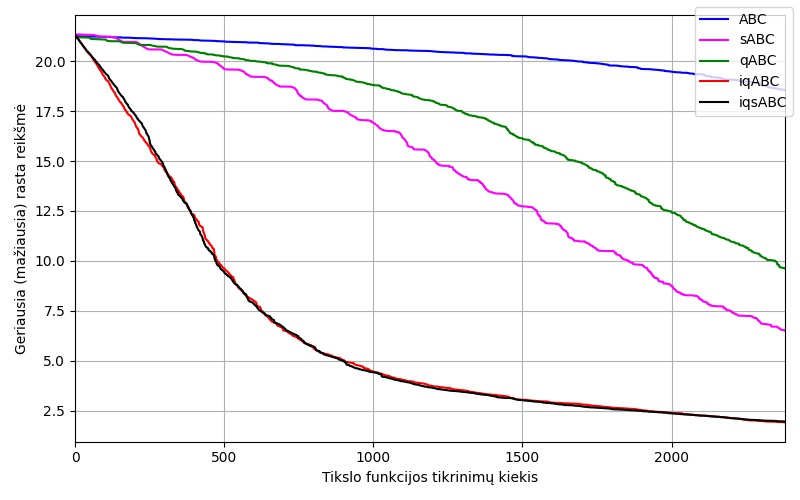
\includegraphics[scale=0.45]{img/2kv/all_ackley.jpg}
    \caption{Algoritmų konvergavimas su Ackley tikslo funkcija}
    \label{img:kon1}
\end{figure}

\begin{figure}[H]
    \centering
    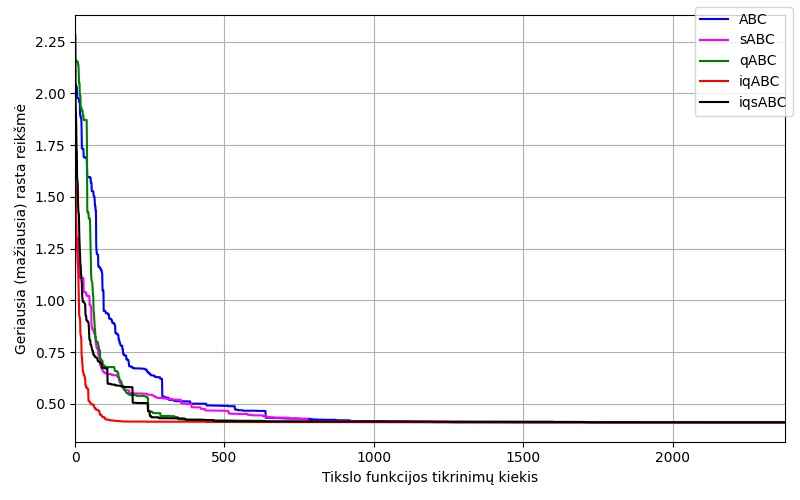
\includegraphics[scale=0.45]{img/2kv/all_branin.jpg}
     \caption{Algoritmų konvergavimas su Branin tikslo funkcija}
    \label{img:kon2}
\end{figure}

\end{multicols}
\begin{multicols}{2}

\begin{figure}[H]
    \centering
    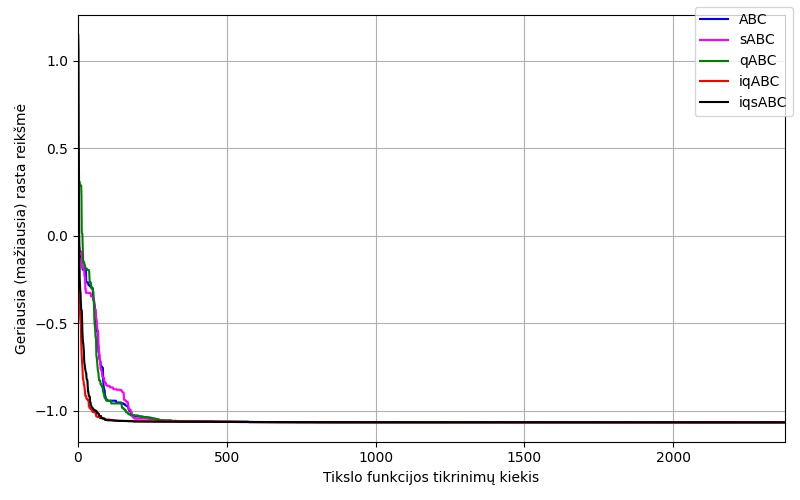
\includegraphics[scale=0.45]{img/2kv/all_camel.jpg}
     \caption{Algoritmų konvergavimas su kupranugario tikslo funkcija}
    \label{img:kon3}
\end{figure}

\begin{figure}[H]
    \centering
    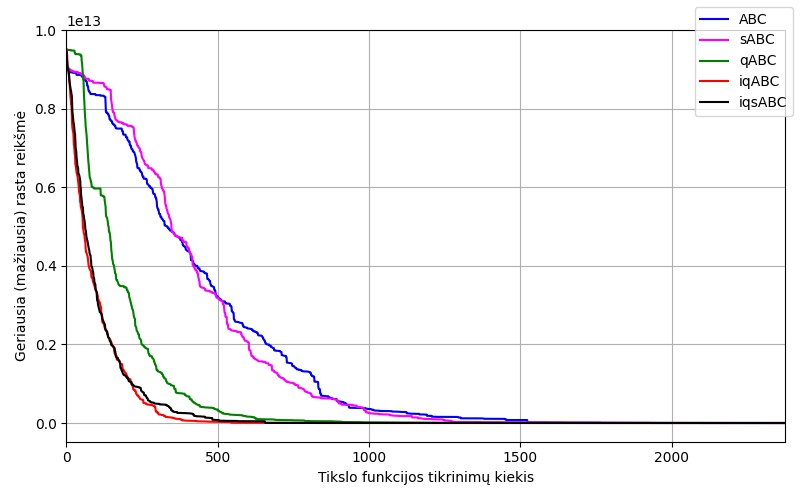
\includegraphics[scale=0.45]{img/2kv/all_dixon.jpg}
     \caption{Algoritmų konvergavimas su Dixon tikslo funkcija}
    \label{img:kon4}
\end{figure}

\end{multicols}\newpage
\begin{multicols}{2}

\begin{figure}[H]
    \centering
    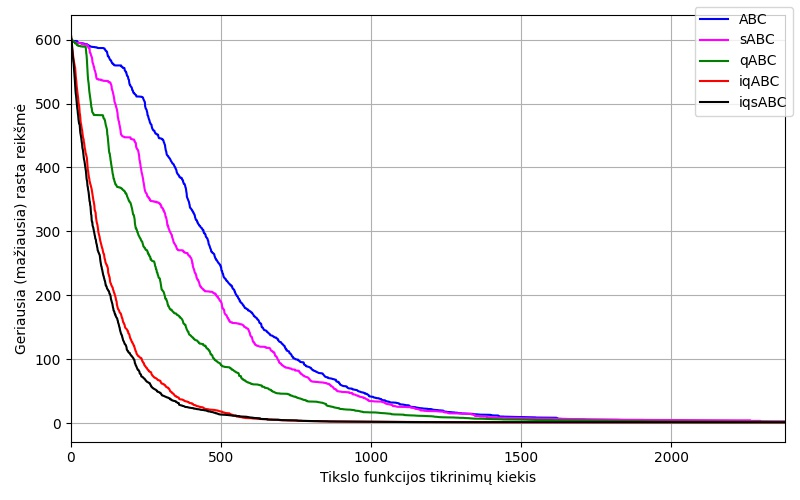
\includegraphics[scale=0.45]{img/2kv/all_griewank.jpg}
     \caption{Algoritmų konvergavimas su Griewank tikslo funkcija}
    \label{img:kon5a}
\end{figure}

\begin{figure}[H]
    \centering
    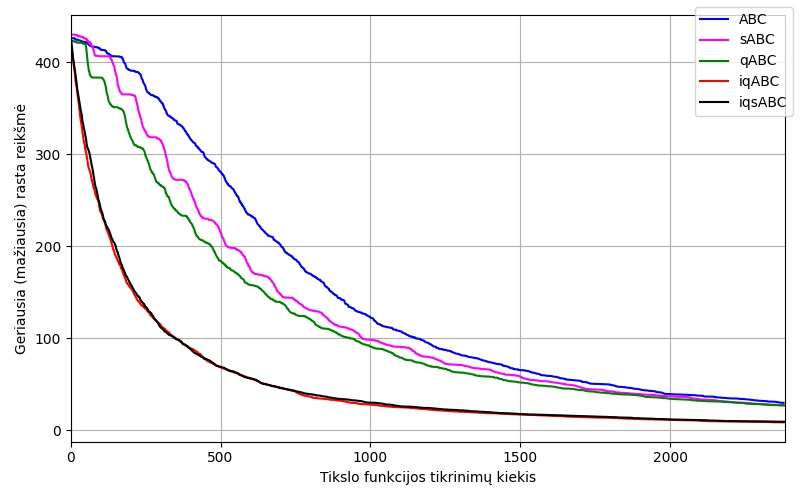
\includegraphics[scale=0.45]{img/2kv/all_rastrigin.jpg}
     \caption{Algoritmų konvergavimas su Rastrigin tikslo funkcija}
    \label{img:kon5}
\end{figure}



\end{multicols}
\begin{multicols}{2}

\begin{figure}[H]
    \centering
    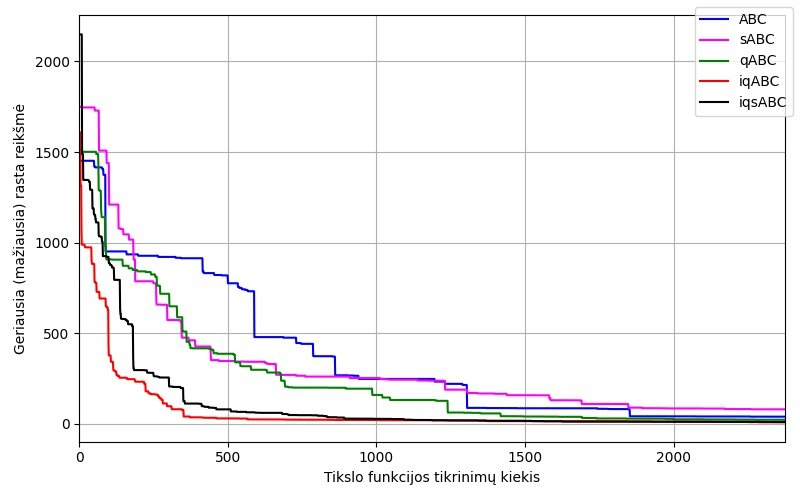
\includegraphics[scale=0.45]{img/2kv/all_rosenbrock.jpg}
     \caption{Algoritmų konvergavimas su Rosenbrock tikslo funkcija}
    \label{img:kon6}
\end{figure}

\begin{figure}[H]
    \centering
    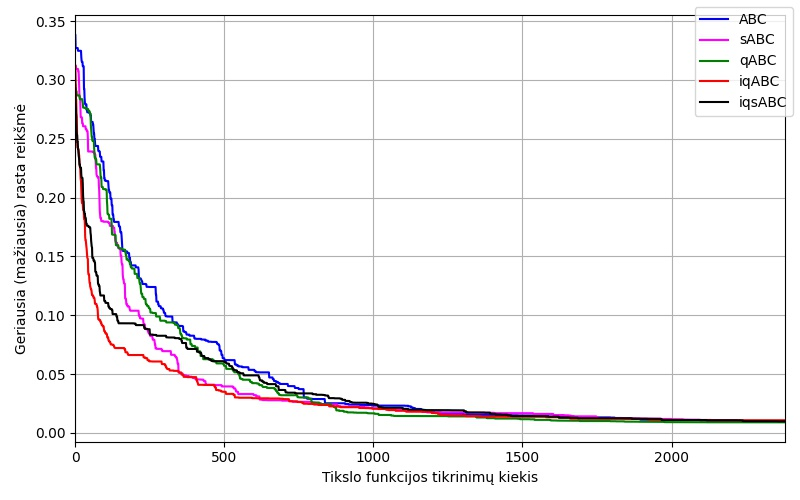
\includegraphics[scale=0.45]{img/2kv/all_schaffer.jpg}
     \caption{Algoritmų konvergavimas su Schaffer tikslo funkcija}
    \label{img:kon7a}
\end{figure}





\end{multicols}\newpage
\begin{multicols}{2}

\begin{figure}[H]
    \centering
    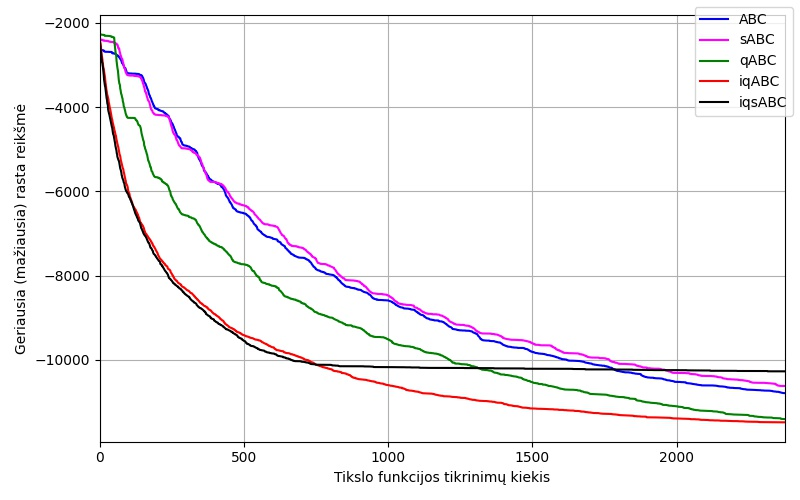
\includegraphics[scale=0.45]{img/2kv/all_schwefel.jpg}
     \caption{Algoritmų konvergavimas su Schwefel tikslo funkcija}
    \label{img:kon7}
\end{figure}

\begin{figure}[H]
    \centering
    \includegraphics[scale=0.45]{img/2kv/all_Sphere.jpg}
     \caption{Algoritmų konvergavimas su sferos tikslo funkcija}
    \label{img:kon8}
\end{figure}





\end{multicols}
\begin{multicols}{2}

\begin{figure}[H]
    \centering
    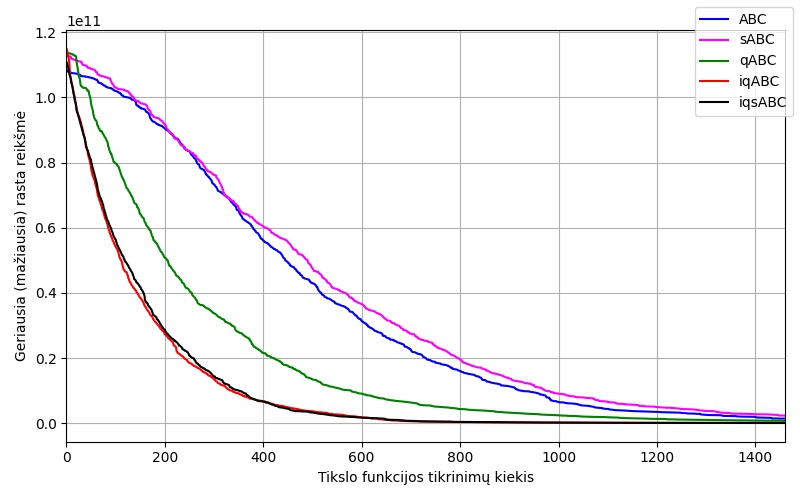
\includegraphics[scale=0.45]{img/2kv/all_f1.jpg}
    \caption{Algoritmų konvergavimas su $f_{1}$ tikslo funkcija}
    \label{img:konf1}
\end{figure}

\begin{figure}[H]
    \centering
    \includegraphics[scale=0.45]{img/2kv/all_f2.jpg}
    \caption{Algoritmų konvergavimas su $f_{2}$ tikslo funkcija}
    \label{img:konf2}
\end{figure}





\end{multicols}\newpage
\begin{multicols}{2}

\begin{figure}[H]
    \centering
    \includegraphics[scale=0.45]{img/2kv/all_f3.jpg}
    \caption{Algoritmų konvergavimas su $f_{3}$ tikslo funkcija}
    \label{img:konf3}
\end{figure}


\begin{figure}[H]
    \centering
    \includegraphics[scale=0.45]{img/2kv/all_f4.jpg}
    \caption{Algoritmų konvergavimas su $f_{4}$ tikslo funkcija}
    \label{img:konf4}
\end{figure}






\end{multicols}
\begin{multicols}{2}

\begin{figure}[H]
    \centering
    \includegraphics[scale=0.45]{img/2kv/all_f5.jpg}
    \caption{Algoritmų konvergavimas su $f_{5}$ tikslo funkcija}
    \label{img:konf5}
\end{figure}

\begin{figure}[H]
    \centering
    \includegraphics[scale=0.45]{img/2kv/all_f6.jpg}
    \caption{Algoritmų konvergavimas su $f_{6}$ tikslo funkcija}
    \label{img:konf6}
\end{figure}





\end{multicols}\newpage
\begin{multicols}{2}

\begin{figure}[H]
    \centering
    \includegraphics[scale=0.45]{img/2kv/all_f7.jpg}
    \caption{Algoritmų konvergavimas su $f_{7}$ tikslo funkcija}
    \label{img:konf7}
\end{figure}


\begin{figure}[H]
    \centering
    \includegraphics[scale=0.45]{img/2kv/all_f8.jpg}
    \caption{Algoritmų konvergavimas su $f_{8}$ tikslo funkcija}
    \label{img:konf8}
\end{figure}





\end{multicols}
\begin{multicols}{2}

\begin{figure}[H]
    \centering
    \includegraphics[scale=0.45]{img/2kv/all_f9.jpg}
    \caption{Algoritmų konvergavimas su $f_{9}$ tikslo funkcija}
    \label{img:konf9}
\end{figure}



\begin{figure}[H]
    \centering
    \includegraphics[scale=0.45]{img/2kv/all_f10.jpg}
    \caption{Algoritmų konvergavimas su $f_{10}$ tikslo funkcija}
    \label{img:konf10}
\end{figure}



\end{multicols}\newpage
\begin{multicols}{2}

\begin{figure}[H]
    \centering
    \includegraphics[scale=0.45]{img/2kv/all_f11.jpg}
    \caption{Algoritmų konvergavimas su $f_{11}$ tikslo funkcija}
    \label{img:konf11}
\end{figure}



\begin{figure}[H]
    \centering
    \includegraphics[scale=0.45]{img/2kv/all_f12.jpg}
    \caption{Algoritmų konvergavimas su $f_{12}$ tikslo funkcija}
    \label{img:konf12}
\end{figure}






\end{multicols}
\begin{multicols}{2}


\begin{figure}[H]
    \centering
    \includegraphics[scale=0.45]{img/2kv/all_f13.jpg}
    \caption{Algoritmų konvergavimas su $f_{13}$ tikslo funkcija}
    \label{img:konf13}
\end{figure}

\begin{figure}[H]
    \centering
    \includegraphics[scale=0.45]{img/2kv/all_f14.jpg}
    \caption{Algoritmų konvergavimas su $f_{14}$ tikslo funkcija}
    \label{img:konf14}
\end{figure}


\end{multicols}

\begin{figure}[H]
    \centering
    \includegraphics[scale=0.45]{img/2kv/all_f15.jpg}
    \caption{Algoritmų konvergavimas su $f_{15}$ tikslo funkcija}
    \label{img:konf15}
\end{figure}


\end{landscape}





\section{Landšafto tikslo funkcijos grafikai}\label{PR4goal}

\begin{figure}[H]
    \centering
    \includegraphics[scale=0.8]{img/new/fitres.png}
    \caption{Tikslo funkcijos pritaikymo landšafto informacijai reikšmių atvaizdavimas}
    \label{mapgoalpic}
\end{figure}



\section{Pseudokodai}\label{PR5pseudo}


\begin{algorithm}[H]
\floatname{algorithm}{}
\caption{\textbf{algoritmas:} Stebinčios bitės iqsABC algoritmo žingsnio pseudokodas}
\begin{spacing}{1.0}
\begin{algorithmic}[1]
    \ForAll{$i \gets SN $}
        \State $p(x_i) \gets \text{tikimybė iš \eqref{iqssp}}$
    \EndFor
    \State $visosBites \gets 1$
    \State $pasirinktaBite \gets 1$
    \While{$visosBites < SN \And visiIvertinimai \leq maxIvertinimai$}
        \If{$rand(0,1) \leq p_{santykinis}(x_{pasirinktaBite}) $}
            \If{$bandymai_{stebinciu} \leq l_{santykinis}(x_{isimintas}) $}
                \State $i_{isimintas} \gets \text{geriausio sprendinio indeksas} $
                \State $x_{isimintas} \gets  \text{geriausio sprendinio vektorius} $
                \State $v_{naujas} \gets \text{naujo sprendinio vektorius pagal \eqref{eiqabcobp} } $
                \If{$fit(x_{isimintas}) \geq fit(v_{naujas}) $}
                    \State $x_{isimintas} \gets v_{naujas}$
                    \State $bandymai(x_{isimintas}) \gets 0$
                \Else
                    \State $bandymai(x_{isimintas}) \gets bandymai(x_{isimintas})+1$
                    \State $bandymai_{stebinciu} \gets bandymai_{stebinciu}+1$
                \EndIf
                

            \Else      
                \State $v_{naujas} \gets \text{naujo sprendinio vektorius pagal} \eqref{eebp1}$
                \If{$fit(x_{pasirinktaBite}) \geq fit(v_{naujas}) $}
                    \State $pasirinktaBite \gets v_{i} $
                    \State $bandymai(pasirinktaBite) \gets 1$
                \Else
                    \State $bandymai(pasirinktaBite) \gets bandymai(pasirinktaBite)+1$
                \EndIf
            \EndIf
        \State $visiIvertinimai \gets visiIvertinimai + 1$
        \State $visosBites \gets visosBites + 1$
        \EndIf
        \State $pasirinktaBite \gets pasirinktaBite+1$
        \If{$pasirinktaBite \geq SN$}
            \State $pasirinktaBite \gets 1$
        \EndIf
    \EndWhile
\end{algorithmic}
\end{spacing}
\label{alg:1}
\end{algorithm}

\begin{algorithm}[H]
\floatname{algorithm}{}
\caption{\textbf{algoritmas:} Dirbančios bitės iqsABC algoritmo žingsnio pseudokodas}
\begin{spacing}{1.0}
\begin{algorithmic}[1]
    \ForAll{$i \gets SN $}
        \If{$rand(0,1) \leq p(x_{pasirinktaBite}) $}
            \If{$bandymai_{darbininkiu} \leq l_{santykinis}(x_{isimintas}) $}
                \State $i_{isimintas} \gets \text{geriausio sprendinio indeksas} $
                \State $x_{isimintas} \gets  \text{geriausio sprendinio vektorius} $
                \State $v_{naujas} \gets \text{naujo sprendinio vektorius pagal \eqref{eiqabcebp} } $
                \If{$fit(x_{isimintas}) \geq fit(v_{naujas}) $}
                    \State $x_{isimintas} \gets v_{naujas}$
                    \State $bandymai(x_{isimintas}) \gets 0$
                \Else
                    \State $bandymai(x_{isimintas}) \gets bandymai(x_{isimintas})+1$
                    \State $bandymai_{darbininkiu} \gets bandymai_{darbininkiu}+1$
                \EndIf
                

            \Else      
                \State $v_{naujas} \gets \text{naujo sprendinio vektorius pagal} \eqref{eebp1}$
                \If{$fit(x_{pasirinktaBite}) \geq fit(v_{naujas}) $}
                    \State $pasirinktaBite \gets v_{i} $
                    \State $bandymai(pasirinktaBite) \gets 1$
                \Else
                    \State $bandymai(pasirinktaBite) \gets bandymai(pasirinktaBite)+1$
                \EndIf
            \EndIf
        \EndIf
        \State $visiIvertinimai \gets visiIvertinimai + 1$
    \EndFor
\end{algorithmic}
\end{spacing}
\label{alg:2}
\end{algorithm}





\end{document}








